\documentclass[12pt, oneside]{book}
%------------------------------Zone 1-------------------------
\usepackage[utf8]{inputenc} % Required for inputting international characters
\usepackage[T1]{fontenc} % un second package permettant d'utiliser tous les caractères de votre clavier.
\usepackage[francais]{babel} % un troisième package pour dire à <em>Latex</em> que vous écrivez en français.
\AddThinSpaceBeforeFootnotes % à insérer si on utilise \usepackage[french]{babel}
\FrenchFootnotes % à insérer si on utilise \usepackage[french]{babel}
 \usepackage{amsmath}
\usepackage{amsfonts}
\usepackage{amssymb}
\usepackage{float}
\usepackage{graphicx}
\usepackage{amsthm}
\usepackage{tikz}
\usepackage[hmargin=3 cm,vmargin= 3 cm]{geometry}
\usepackage[toc,page]{appendix} 
\usepackage[Glenn]{fncychap}
\usepackage{fancyhdr}
%\usepackage{titlesec}
\usepackage{minitoc}
%\usepackage{french} 
\usepackage{array,multirow,makecell}
\usepackage{lettrine}
\usepackage{caption}
\DeclareCaptionFormat{sanslabel}{#3}%
%------------------------------Fin Zone 1---------------------------
% Interligne
\usepackage{setspace}
% \singlespacing
\onehalfspacing
% \doublespacing
\usepackage{hyperref}
\usepackage{diagbox}
\begin{document}
%------------------------------Zone 2: début des page non numérotées-------------------------
\frontmatter
\begin{titlepage}
\begin{center}
%\large
\vspace{-2.5 cm}
{ \large \textbf {République Algérienne Démocratique et Populaire}  \\
\normalsize \textbf{Ministère de l'Enseignement Supérieur et de la Recherche Scientifique}} \\
{ \large \textbf {Université Batna 2 - Mostafa Ben Boulaïd -}\\
%\vspace{-0.3cm}

\begin{tabular}{l m{12 cm} l}
  
\includegraphics[scale=0.15]{PageDeGarde/lg.png}& 
   \centering{\textbf{Faculté des mathématiques et de l'informatique  Département d'informatique}}
  & 
\includegraphics[scale=0.15]{PageDeGarde/lg.png}\\
  
\end{tabular}\\
}
\vspace{2cm}
\Huge{\textbf{Mémoire }}\\
\normalsize{Présenté }\\
 \normalsize\textbf{Pour l'obtention du grade de Master en Informatique }\\
\textit{ \normalsize{Option: Intelligence Artificielle et Multimédia }}\\
\Large\textbf{{Thème}}\\
\vspace{0.5cm}
\begin{tabular}{||c||}
  \hline
  \\
  \large\textbf{Deep learning pour la détection d'objets}\\ 
  \\
   %\large\textbf{ }\\
   \hline
\end{tabular}\\
\vspace{0.5cm}
\normalsize \textbf{Présenté par: }\\
\large{ ZEROUAL Aymene }\\
\large{ ZEROUAL Wail}\\
\vspace{1cm}
\begin{tabular}{l p{5 cm} }
  \normalsize\textbf{Dirigé par: }& \normalsize{Dr. Leïla BOUSSAAD } \\
 \end{tabular}\\
\vspace{2.2 cm}
\normalsize \textbf{Promotion: 2022/2023 }
\end{center}
\end{titlepage}
%\newpage
\thispagestyle{empty}
\begin{center}
\textcolor[rgb]{0,0,1}{{\Huge\textbf{\textit{Remerciements}}}}
\end{center}

\vspace{1 cm}

\begin{center}
Nous tenons à remercier avant tout, ALLAH qui nous a donné la force, la capacité et la patience d'effectuer ce  modeste travail.

Nous tenons à remercier Madame Leïla BOUSSAAD et Madame Aldjia BOUCETTA pour avoir accepté de diriger et encadrer ce projet de fin d'études et aussi pour leur disponibilité et leurs précieux conseils qui m'ont permis de réussir ce travail.

Nous tenons également à exprimer toute notre gratitude à Monsieur Moumen HAMOUMA,  Maître de conférence, Université Batna 2, de nous avoir fait l'honneur d'accepter la présidence du jury de notre soutenance.

Nous adressons également nos sincères remerciements à Monsieur  Badreddine BENREGUIA, Maître de conférence, université Batna 2, pour avoir accepté d'évaluer ce travail.

Enfin nous adressons nos remerciements les plus sincères à tous ceux qui ont contribué de près ou de loin à la réalisation de ce travail.
\end{center}
%\newpage
\thispagestyle{empty}
\begin{center}
\textcolor[rgb]{0,0,1}{{\Huge\textbf{\textit{Dédicaces}}}}
\end{center}

\vspace{1 cm}

\begin{center}
\textcolor[rgb]{0,0,1}{\textit{******************* \hspace{0.5 cm}\LARGE{\textbf{K}outaiba}} \hspace{0.5 cm}  \textit{*******************}}\\
\textit{\textbf{A} mes très chers parents pour leur amour inestimable, leur confiance, leur soutien, leurs sacrifices et toutes les valeurs qu'ils ont su m'inculquer. }\\
\textit{\textbf{A} Mes frères : Sofiane, Abdeljalil, Abdelmoiz}\\
\textit{\textbf{A} Mes Sœurs : Meriem, Inchirah, Abrar}\\
\textit{\textbf{A} Ma fiancée : Aya }\\
\textit{\textbf{A} Mes Amis :Bilel , Ala , Kamel , Aymen, Hasni}\\
\textit{\textbf{A} Mon binôme Amine et sa famille }\\
\textit{\textbf{A} tous mes amis de l'Université et d'ailleurs }\\
\textit{\textbf{A} toute personne ayant contribué à ce travail de près ou de loin.}\\
\end{center}
\vspace{1 cm}

\begin{center}
\textcolor[rgb]{0,0,1}{\textit{******************* \hspace{0.5 cm}\LARGE{\textbf{A}mine}} \hspace{0.5 cm}  \textit{*******************}}\\
\textit{\textbf{J}e voudrais dédier ce travail à toute ma famille.}\\
\textit{\textbf{M}a chère maman et mon cher père.}\\
\textit{\textbf{M}es sœurs et mon frère.}\\
\textit{\textbf{M}on ami Koutaiba Belagrouz et sa famille.}\\
\textit{\textbf{T}ous mes amis à travers les années.}\\
\textit{\textbf{M}erci d’être toujours là pour moi.}\\

\end{center}





%%\chapter*{Résumé} 
\newpage
\thispagestyle{empty}
\begin{center}
{\Large \textbf{Résumé}}
\end{center}
%

La détection d'objets est une technique importante dans le domaine de la vision par ordinateur, car elle est considérée comme étape nécessaire dans n'importe quel processus de reconnaissance. C'est la procédure consistant à déterminer l'instance de la classe à laquelle appartient l'objet et à estimer son emplacement en affichant sa boîte englobante. 

Il est largement approuvé que les progrès de la détection d'objets ont généralement traversé deux périodes historiques : "la période de détection d'objets traditionnelle (avant 2014)", où la détection  a été effectuée grâce à des techniques classiques d'apprentissage automatique, et "la période de détection basée sur l'apprentissage profond (après 2014)", où les techniques classiques d'apprentissage automatique ont été complètement remplacées par des méthodes basées sur des réseaux de neurones profonds. 

Dans ce mémoire,nous nous concentrerons sur la détection d'objet basée sur l'apprentissage profond. L'objectif principal  est de réaliser une étude comparative de trois modèles de la famille YOLO,  déjà prouvés leur efficacité dans ce domaine de détection d'objets, qui sont YOLOv3, YOLOv4 et YOLOv5 dans le contexte de la détection des URL dans des photos prises par un téléphone mobile. 

Les résultats expérimentaux exprimés en terme de précision moyenne, ont montré la capacité de généralisation des trois   modèles YOLOv3, YOLOv4 et YOLOv5, en plus, la stabilité du modèle YOLOV4 vis à vis plusieurs difficultés rajoutées aux images.

\vspace{0.5cm}
\textbf{Mots clés}: Détection d'objets, Apprentissage profond, Réseaux de neurones convolutifs (CNN), YOLO, détection d'URL.
%%\chapter*{Abstract}
\newpage
\thispagestyle{empty}
\begin{center}
{\Large \textbf{Abstract}}
\end{center}
..........

\vspace{1cm}
\textbf{Keywords}: ...




%\dominitoc
\pagenumbering{roman}%numérotation avec les chiffres romains
\setcounter{page}{1} %début de la numérotation est 1.
\addcontentsline{toc}{chapter}{Remerciements}
%\newpage
\thispagestyle{empty}
\begin{center}
\textcolor[rgb]{0,0,1}{{\Huge\textbf{\textit{Remerciements}}}}
\end{center}

\vspace{1 cm}


Nous tenons à remercier avant tout, \textbf{ALLAH} qui nous a donné la force, la capacité et la patience d'effectuer ce  modeste travail.\\

Nous tenons à remercier Madame \textbf{Leïla BOUSSAAD} pour avoir accepté de diriger et encadrer ce projet de fin d'études et aussi pour leur disponibilité et leurs précieux conseils qui nous ont permis de réussir ce travail.\\

Nous tenons également à exprimer toute notre gratitude à Monsieur \textbf{ Abederrezak BENYAHIA},  Maître de conférence, Université Batna 2, de nous avoir fait l'honneur d'accepter la présidence du jury de notre soutenance.\\

Nous adressons également nos sincères remerciements à Madame  \textbf{Aldjia BOUCETTA}, Maître de conférence, université Batna 1, pour avoir accepté d'évaluer ce travail.\\

Enfin nous adressons nos remerciements les plus sincères à tous ceux qui ont contribué de près ou de loin à la réalisation de ce travail.\\


\addcontentsline{toc}{chapter}{Résumé}
%%\chapter*{Résumé} 
\newpage
\thispagestyle{empty}
\begin{center}
{\Large \textbf{Résumé}}
\end{center}
%

La détection d'objets est une technique importante dans le domaine de la vision par ordinateur, car elle est considérée comme étape nécessaire dans n'importe quel processus de reconnaissance. C'est la procédure consistant à déterminer l'instance de la classe à laquelle appartient l'objet et à estimer son emplacement en affichant sa boîte englobante. 

Il est largement approuvé que les progrès de la détection d'objets ont généralement traversé deux périodes historiques : "la période de détection d'objets traditionnelle (avant 2014)", où la détection  a été effectuée grâce à des techniques classiques d'apprentissage automatique, et "la période de détection basée sur l'apprentissage profond (après 2014)", où les techniques classiques d'apprentissage automatique ont été complètement remplacées par des méthodes basées sur des réseaux de neurones profonds. 

Dans ce mémoire,nous nous concentrerons sur la détection d'objet basée sur l'apprentissage profond. L'objectif principal  est de réaliser une étude comparative de trois modèles de la famille YOLO,  déjà prouvés leur efficacité dans ce domaine de détection d'objets, qui sont YOLOv3, YOLOv4 et YOLOv5 dans le contexte de la détection des URL dans des photos prises par un téléphone mobile. 

Les résultats expérimentaux exprimés en terme de précision moyenne, ont montré la capacité de généralisation des trois   modèles YOLOv3, YOLOv4 et YOLOv5, en plus, la stabilité du modèle YOLOV4 vis à vis plusieurs difficultés rajoutées aux images.

\vspace{0.5cm}
\textbf{Mots clés}: Détection d'objets, Apprentissage profond, Réseaux de neurones convolutifs (CNN), YOLO, détection d'URL.
\addcontentsline{toc}{chapter}{Abstract}
%%\chapter*{Abstract}
\newpage
\thispagestyle{empty}
\begin{center}
{\Large \textbf{Abstract}}
\end{center}
..........

\vspace{1cm}
\textbf{Keywords}: ...



\addcontentsline{toc}{chapter}{Liste des tableaux}
\listoftables
\addcontentsline{toc}{chapter}{Table des figures}
\listoffigures
\dominitoc
\tableofcontents

%\input{ListeDesAbreviations/ListeDesAbreviations.tex} % rajoute la liste des abréviations.
%\addcontentsline{toc}{chapter}{Liste des abréviations}

\mainmatter
%\pagenumbering{arabic}% numérotation avec les chiffres arabe
%\setcounter{page}{1} % début de la numérotation est 1.
%\addcontentsline{toc}{chapter}{Introduction générale}
\chapter*{Introduction générale}
\newpage
\pagestyle{fancy}
\fancyhead[L]{}
\fancyhead[R]{Introduction générale}
\renewcommand{\headrulewidth}{1pt}
\fancyfoot[C]{\thepage}


\section*{Introduction}
La détection d'objets comme étape principale dans n'importe quel processus  de reconnaissance, est la procédure consistant à déterminer l'instance de la classe à laquelle appartient l'objet et à estimer l'emplacement de l'objet en affichant le cadre de délimitation autour de l'objet. La détection d'une instance unique de classe à partir d'une image est appelée détection d'objet à classe unique, tandis que la détection des classes de tous les objets présents dans l'image est connue sous le nom de détection d'objet multi-classes. 

Récemment, la détection d'objets basée sur l'apprentissage profond a atteint de très bonnes performances. Cependant, il existe de nombreux défis avec les images prises dans le monde réel, tels que le bruit, l'occlusion partielle/complète, les conditions d'éclairage, la pose, etc. Ces problèmes ont un impact important sur la détection des objets et doivent être traités lors de la détection d'objet. 

L'objectif principal de ce mémoire est d'exploiter le domaine de l'apprentissage profond et son application à la détection d'objets. Puis, en utilisant des panneaux de signalisation comme exemple, le but principal de ce mémoire est d'implémenter et d'évaluer les performances du modèle YOLO pour divers situations, en appliquant des techniques de traitement d'images traditionnelles pour simuler les problèmes existant dans les images prises dans scènes réelles.

\section*{Structure du document}
Le mémoire est composé de trois chapitres et une conclusion:

\begin{itemize}
\item Le premier chapitre introduit le domaine de la détection d'objets.
\item Le deuxième chapitre est consacré à la détection d'objets en utilisant les outils de l'apprentissage profond. Il présente les principales techniques qui ont été développées dans ce contexte, ainsi que les principales bases d'images et métriques utilisées pour l'évaluation.
\item Le troisième chapitre décrit les différentes expérimentations, ainsi que les résultats obtenus et leur synthèse.
\item La conclusion conclut le travail réalisé et présente les différentes perspectives.
\end{itemize}
 \chapter{La détection d'objets}
\minitoc
\newpage
\pagestyle{fancy}
\fancyhead[L]{\chaptername \ \thechapter}
\fancyhead[R]{La détection d'objets}
\renewcommand{\headrulewidth}{1pt}
\fancyfoot[C]{\thepage}

\section{Introduction} 
La détection d'objet est un sous-domaine de vision par ordinateur dont le but de localiser la position de l'objet recherché et d'identifier en lui attribuant la classe appropriée dans une image numérique. Le besoin de détection d'objets est d'automatiser les tâches difficiles qui nécessitent une intervention humaine ou impossible à faire par l'homme. Par exemple, la tâche de lire le numéro d'immatriculation
de chaque voiture qui passe sur l'autoroute où les voitures passent à grande vitesse que l'œil humain avec le cerveau est incapable de percevoir quelques chiffres, sans parler du numéro d'enregistrement complet.
\section{Objectif}
L'objectif de la détection d'objets est divisé en 2 composants principaux; premièrement, la localisation d'objets et deuxièmement, l'identification ou la classification d'objets.
\subsection{Localisation d'objet}
Ce composant est la principale différence entre la détection d'objet dans l'image et la classification d'image où, dans la classification d'image, l'objet est identifié uniquement sans son emplacement dans l'image, d'autre part, dans la détection d'objet, l'objet est également localisé en utilisant la technique de la boîte englobante ou technique basée sur les pixels qui se divise également en segmentation sémantique et segmentation d'instance.
\subsubsection{Boîte englobante (Bounding Box)}
La technique de la boîte englobante est la méthode traditionnelle d'étiquetage des données dans l'image. Les cadres de délimitation sont des marqueurs d'annotation dessinés autour des objets dans une image. Contours mais en forme de forme rectangulaire. Il a fait l'objet des études les plus approfondies en raison de sa facilité d'utilisation et de calcul.

\begin{figure}[H]
\centering
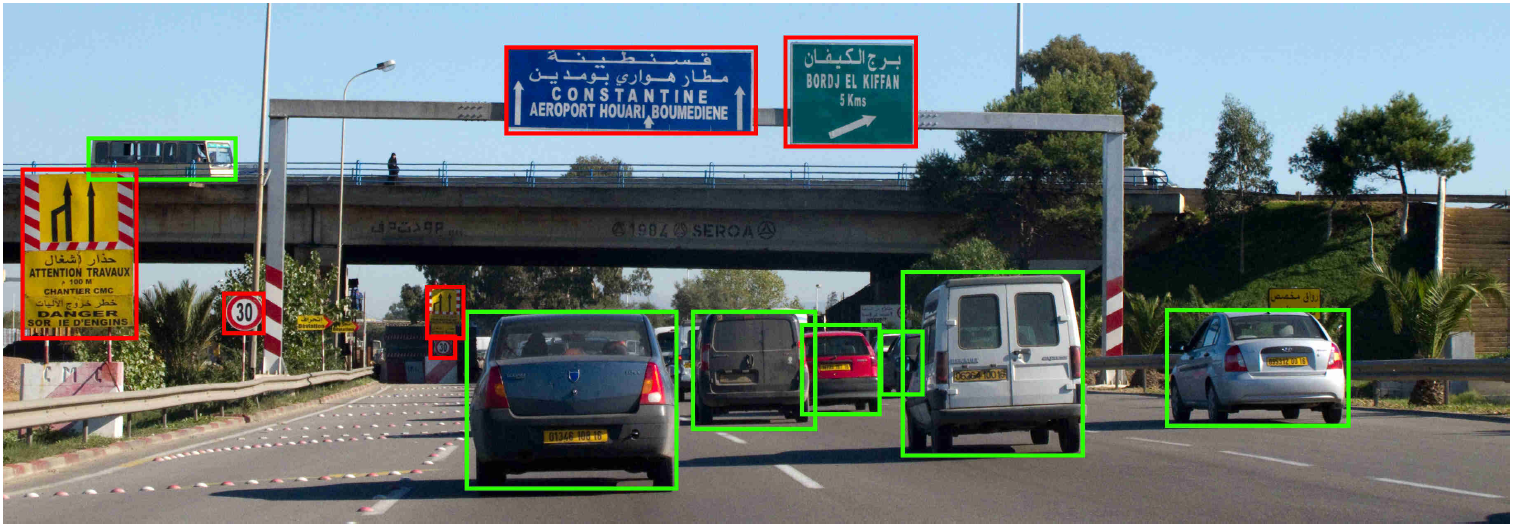
\includegraphics[height=5.7cm,width=16cm]{Chapitre1/im4.png}
\caption{---------.}
\label{im4}
\end{figure}

\subsubsection{Mask (niveau de pixel)}
La deuxième technique utilisée dans la détection d'objets est basée sur les pixels. il nécessite de segmenter l'objet en pixel au lieu de la boîte englobante. cette technique donne un emplacement précis (au niveau du pixel) d'un objet et des pixels trouvés. les pixels produits peuvent aussi être appelés le masque. Il existe 2 types de segmentation, la premier est la segmentation sémantique où tous les objets de la même classe obtiennent le même pixel, où dans le deuxième type, la segmentation d'instance, chaque objet de l'image obtient son masque unique même s'il existe d'autres objets avec la même classe. En raison de la nature de bas niveau de cette technique, elle nécessite une puissance de calcul importante pour segmenter l'objet pixel par pixel, de plus cette technique est assez nouvelle et encore immature en raison des faibles études appliquées dans celle-ci.

\begin{figure}[H]
\centering
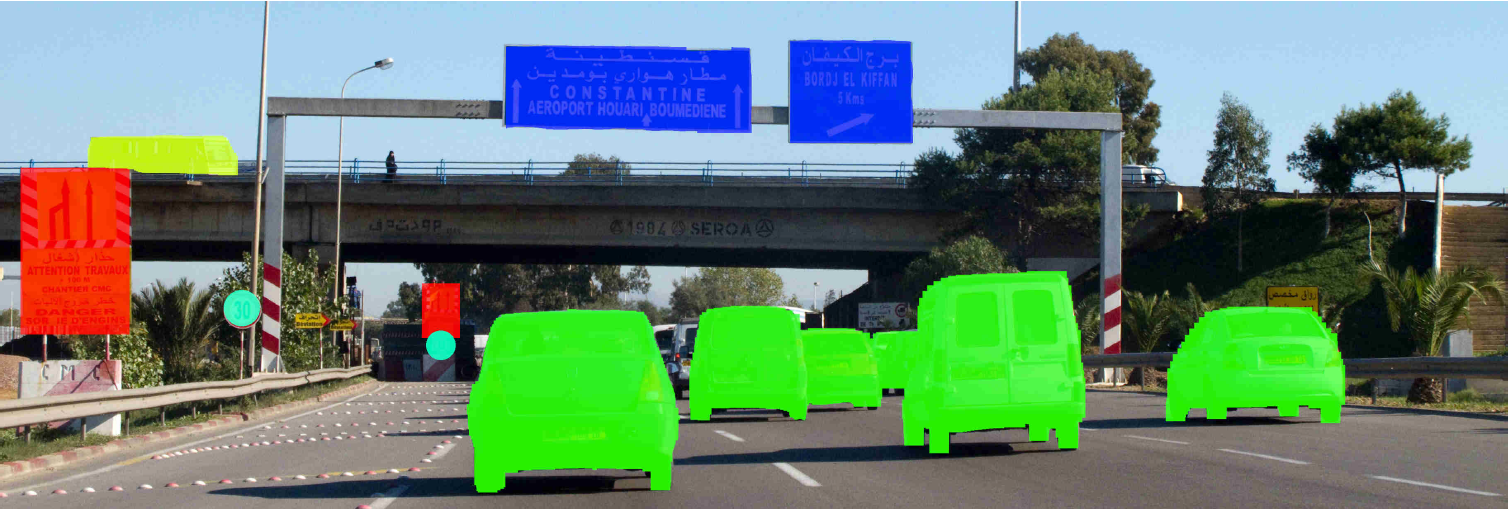
\includegraphics[height=5.7cm,width=16cm]{Chapitre1/im5.png}
\caption{---------.}
\label{im5}
\end{figure}
\begin{figure}[H]
\centering
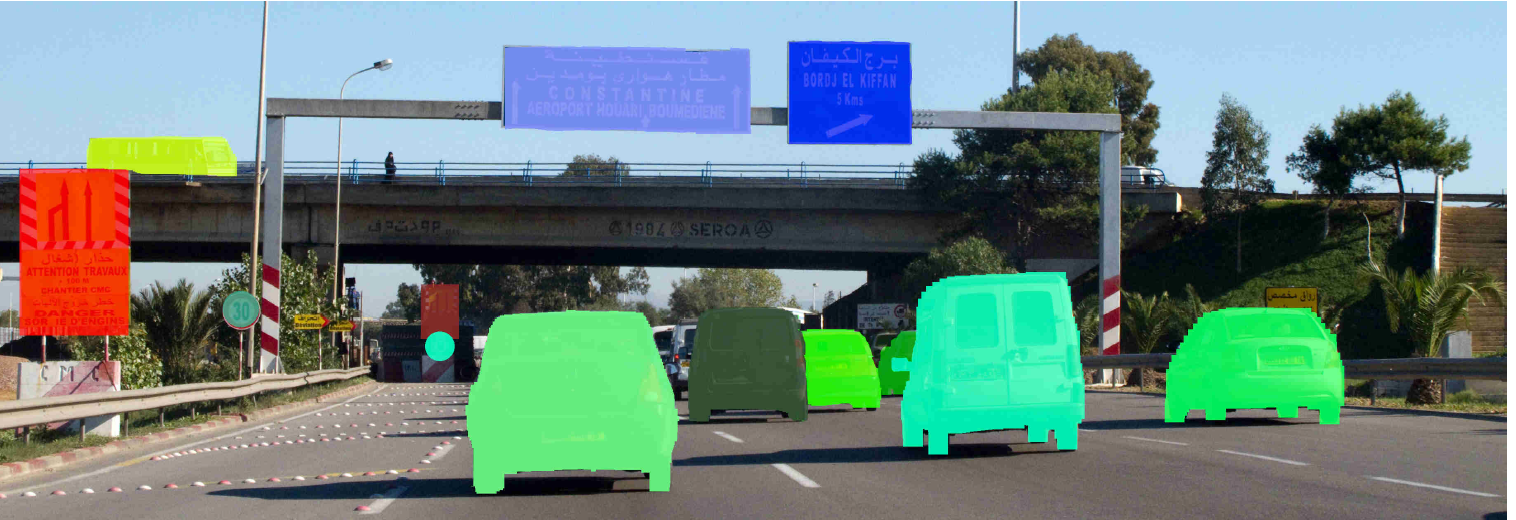
\includegraphics[height=5.7cm,width=16cm]{Chapitre1/im6.png}
\caption{---------.}
\label{im6}
\end{figure}


\subsection{Classification d'objet}
Le deuxième composant est la reconnaissance d'objets. La reconnaissance est la capacité du modèle (le réseau de neurones dans notre cas) à identifier un objet en fonction de certaines similitudes qu'il partage avec un autre objet que le modèle a déjà rencontré. La reconnaissance peut être basée sur une inférence ou une relation, c'est-à-dire une situation dans laquelle un modèle est capable de reconnaître un objet parce qu'il reconnaît les similitudes de
forme et de propriétés. La reconnaissance peut également se produire parce que le modèle a rencontré l'objet exact lors d'une instance précédente Chez les êtres humains, la reconnaissance est un processus cognitif qui se déroule de manière transparente et presque instantanément sans délai. Le cerveau humain est capable d'apprendre et d'adapter des informations avec un minimum d'effort, de sorte que même les humains qui en sont encore aux stades de développement de leur existence peuvent facilement reconnaître les objets. Les humains peuvent reconnaître une multitude d'objets dans des images avec peu d'effort, même si l'image des objets peut varier quelque peu selon différents points de vue, dans de nombreuses tailles et échelles
différentes ou même lorsqu'ils sont déplacés ou pivotés. Les objets peuvent même être reconnus lorsqu'ils sont partiellement masqués. La machine ou le modèle, cependant, ne possède pas de façon innée cette capacité cognitive.
Pour que l'intelligence artificielle acquière ce niveau de compétence, elle doit acquérir une formation. Cette formation est généralement acquise en apprenant les jeux de données du modèle. Cette tâche reste un défi pour les systèmes de vision par ordinateur étant donné que ces modèles doivent être entraînés pour chaque classe d'objets qu'ils sont censés reconnaître.

\begin{figure}[H]
\centering
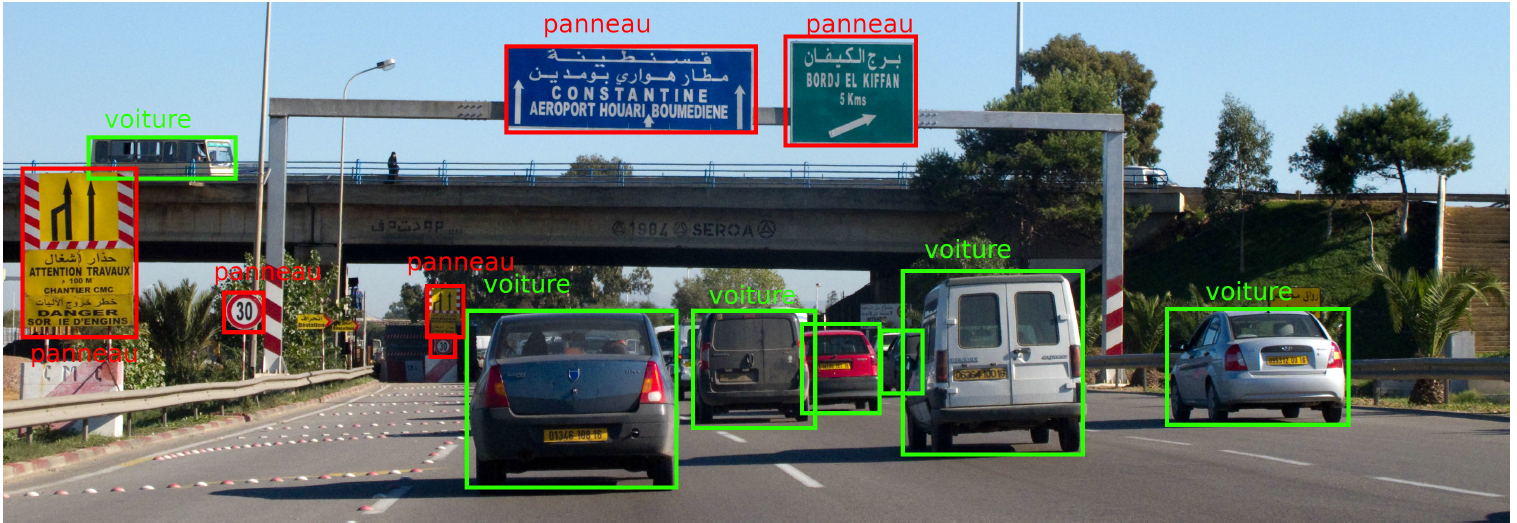
\includegraphics[height=6cm,width=16cm]{Chapitre1/im7.png}
\caption{---------.}
\label{im7}
\end{figure}

\section{Historique}
L'histoire de la détection d'objets est divisée en 2 époques la première époque est nommée l'époque traditionnelle ou l'époque avant l'apprentissage profond où les ressources étaient extrêmement limitées qui incluent la faible puissance de calcul des machines avec le manque de représentation d'image efficace, par conséquent, les algorithmes qui ont été construits à cette époque sont basés sur des caractéristiques sélectionnées manuellement, comme les détecteurs Viola Jones développé par Paul Viola and Michael Jones en 2001
qui permis la détection de visages humains en temps réel à l'aide d'une fenêtre coulissante qui recherche les caractéristiques du visage, malheureusement, la détection d'objets a atteint un plateau après 2010, car les performances des caractéristiques sélectionnées manuellement sont devenues saturées.
Après la généralisation d'Internet dans le monde entier et l'augmentation des données flottant sur le Web qui ont conduit à la création d'ImageNet, une grande base de données visuelle conçue pour être utilisée dans la recherche de logiciels de reconnaissance visuelle d'objets. et l'augmentation drastique de la puissance de calcul des machines provoquée par le développement de systèmes de calcul parallèles comme les super-machines de calcul haute performance (HPC), A ouvert la voie à l'apprentissage profond en particulier aux réseaux de neurones convolutifs (CNN) A ouvert la voie à l'apprentissage en profondeur, en particulier aux réseaux de neurones
convolutifs et le plus célèbre est AlexNet implementé par Alex Krizhevsky en 2012. De nombreux algorithmes sont apparus après pour amélioré les performances et le résultat et nous utiliserons l'algorithme YOLO plus tard.
\section{Etat de l'art des techniques de détection d'objets}

----

 
\section{Les applications de la détection d'objets}
La détection d'objets fait son entrée dans un large éventail d'industries, avec des cas d'utilisation allant de la sécurité personnelle à la productivité sur le lieu de travail. La détection et la reconnaissance d'objets sont appliquées dans de nombreux domaines de la vision par ordinateur, notamment la récupération d'images, la sécurité, la surveillance, les systèmes de véhicules automatisés et l'inspection des machines. Des défis importants subsistent dans le domaine de la reconnaissance d'objets. Les possibilités sont infinies en ce qui concerne les futurs cas d'utilisation de la détection d'objets. Dans cette section, nous discutons  certaines applications actuelles et futures  des systèmes de détection d'objets dans divers domaines..
\subsection{Reconnaissance optique de caractères}

\subsection{Voitures autonomes}

\subsection{Suivi des objets}
Le système de détection d'objets est également utilisé pour suivre les objets, par exemple suivre un ballon pendant un match de football, suivre une personne dans une vidéo. Le suivi d'objets a une variété d'utilisations, dont certaines sont la surveillance et la sécurité , surveillance du trafic, communication vidéo, vision et animation de robots.

\begin{figure}[H]
\centering
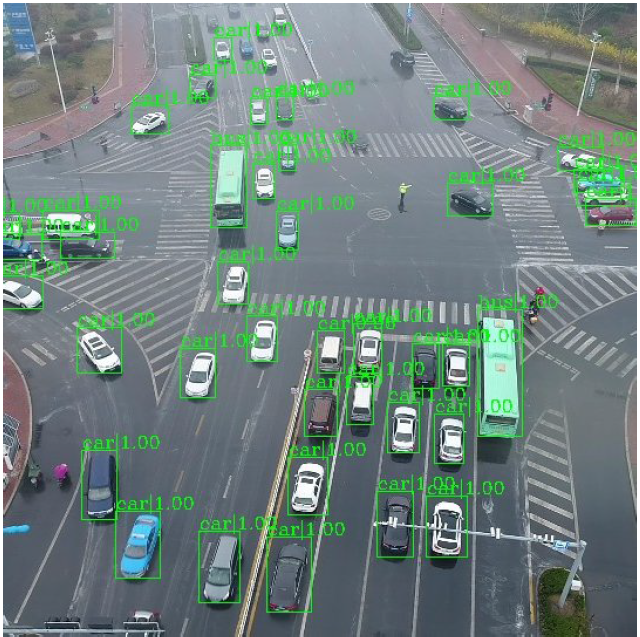
\includegraphics[height=6.5cm,width=6.5cm]{Chapitre1/im10.png}
\caption{---------.}
\label{im10}
\end{figure}

\subsection{Biométrie}

\subsection{reconnaissance d'activités}

\subsection{Tatouage numérique}

\subsection{Imagerie médicale}

\subsection{Robotique}

\subsection{Production industrielle}
Les usines du monde entier s'efforcent de produire des produits de la
meilleure qualité avec un coût de production minimum. Cependant, pour
atteindre cet objectif, les usines doivent embaucher de la main-d'œuvre pour vérifier la qualité des composants, ce qui augmente le coût de production et d'autres problèmes liés au travail manuel. comme la dextérité et la productivité du travailleur. La détection d'objets résout les problèmes liés au travail manuel. il garantit que les bons composants sont utilisés dans les chaînes de montage et que les processus corrects sont suivis avec une précision et une exactitude élevées, plus qu'un travailleur manuel et à moindre coût.

\begin{figure}[H]
\centering
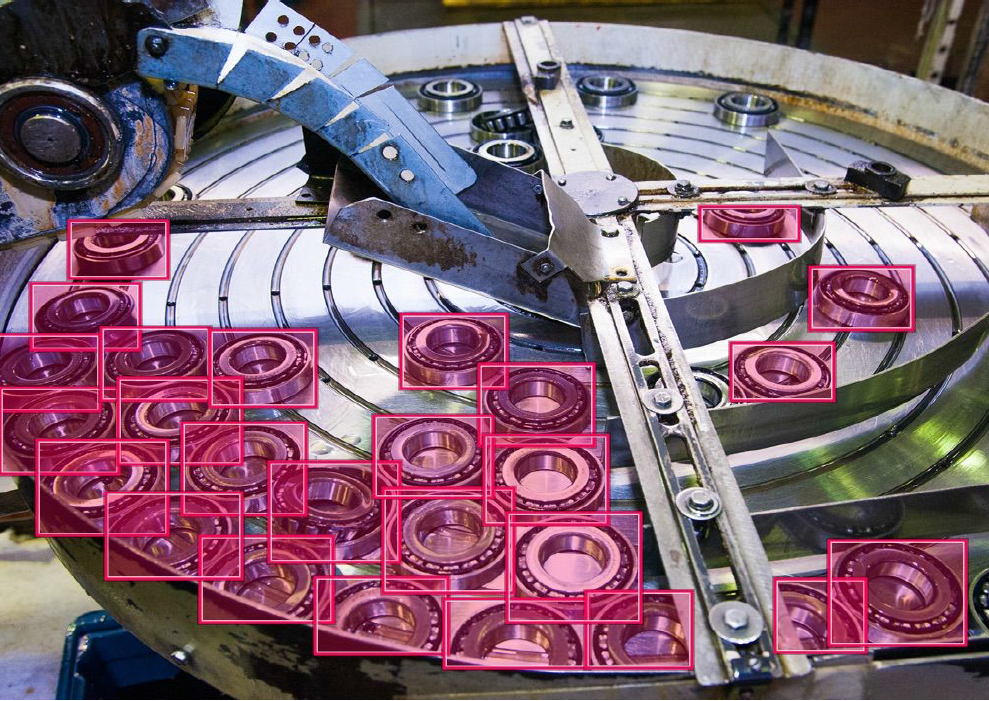
\includegraphics[height=7cm,width=12cm]{Chapitre1/im8.png}
\caption{---------.}
\label{im8}
\end{figure}

\subsection{Surveillance et sécurité}
Dans les grandes villes où la population est très élevée, dans les zones industrielles, les grandes banques et de nombreuses autres zones hautement sensibles, la sécurité est indispensable 24 heures sur 24 et il est presque impossible pour un être humain d'atteindre ce niveau. La détection d'objets est donc une solution à ce type de problèmes où elle suit les mouvements des visiteurs, suit les comportements des individus ou des véhicules, fait la distinction entre les activités autorisées et non autorisées et signale lorsqu'un objet inattendu nécessite une enquête. tout cela 24 heures sur 24 sans arrêt et
aussi à moindre coût de maintenance.

\begin{figure}[H]
\centering
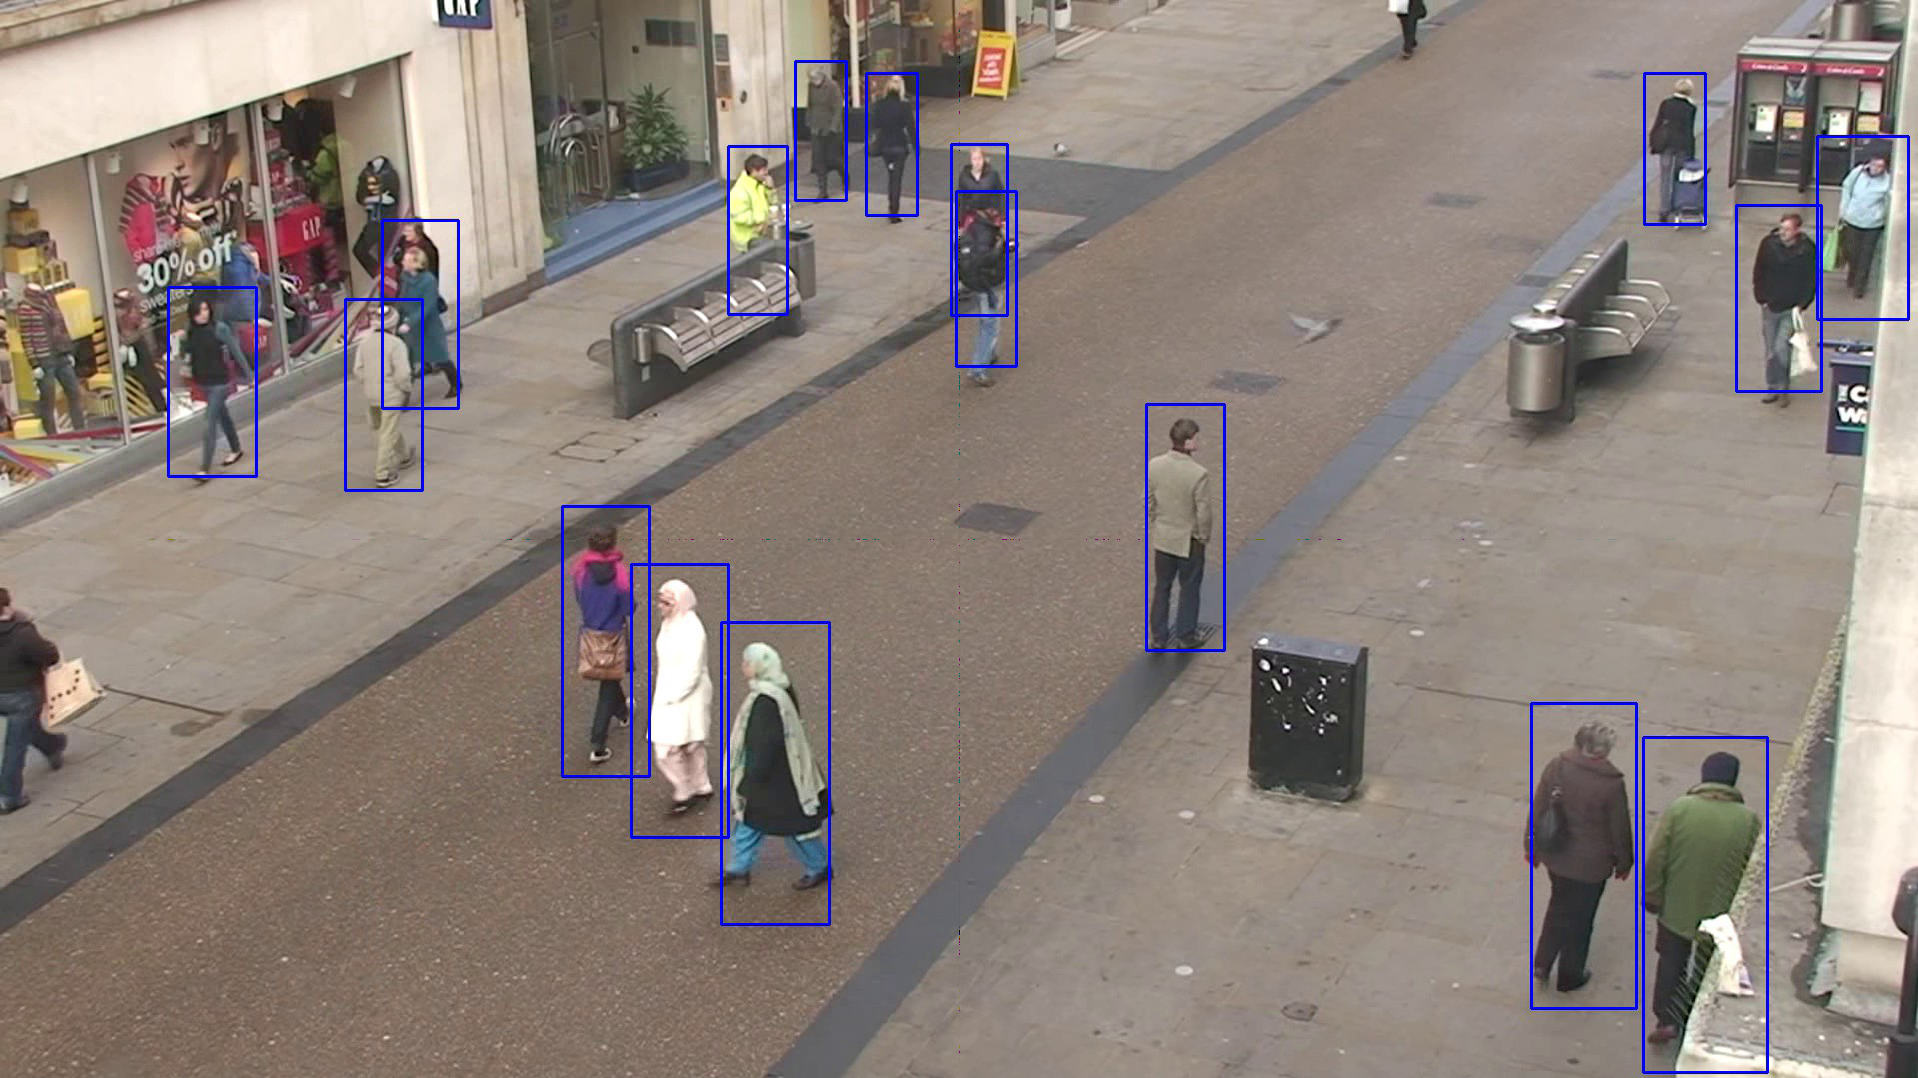
\includegraphics[height=6cm,width=14cm]{Chapitre1/im9.png}
\caption{---------.}
\label{im9}
\end{figure}

\section{Conclusion}


\chapter{Détection d'objets et apprentissage profond}
\newpage
\pagestyle{fancy} 
\fancyhead[L]{\chaptername \ \thechapter}
\fancyhead[R]{Détection d'objets et apprentissage profond}
\renewcommand{\headrulewidth}{1pt}
\fancyfoot[C]{\thepage}
\section{Introduction} 
Malgré la popularité des techniques traditionnelles de vision par ordinateur et d'apprentissage automatique, le développement de l'apprentissage profond a renversé la situation, de sorte que de nombreux problèmes de vision par ordinateur y compris la détection d'objets se sont traités à l'aide d'architectures profondes, généralement des réseaux de neurones convolutifs (CNN) \cite{gupta2014learning}, qui ont pu surpasser les autres approches en termes d'efficience et d'efficacité.

Dans ce chapitre, nous allons introduire les réseaux de neurones convolutifs et exposer certains réseaux convolutifs communs qui sont souvent utilisés comme base pour les systèmes de détection d'objets, et les techniques courantes d'apprentissage telles que l'apprentissage par transfert.

Également, nous présenterons  les différentes bases d'images et métriques utilisées pour l'évaluation. En outre, nous décrirons certaines des méthodes basées sur l'apprentissage profond existantes. 



% =========== CNN =========== 
\section{Les réseaux de neurones convolutifs } 

Un réseau de neurones convolutif (CNN ou ConvNet) est un type de réseau de neurones artificiels acyclique  dans lequel l'architecture des connexions est inspirée de celle du cortex visuel des mammifères \cite{Deep2018}.
 
Un réseau de neurones convolutif  est  distingué des réseaux de neurones classiques entièrement connectés en combinant un certain nombre de couches connectées localement destinées à l'extraction automatique des caractéristiques, suivies d'un nombre de couches entièrement connectées destinées à la classification \cite{Deep2016}.

 Un CNN comprend une succession de couches pour extraire les caractéristiques discriminante, plusieurs couches distinctes,chacune ayant un objectif spécifique, notamment  des couches convolutives, de correction,  des couches de sous-échantillonnage appelées couches de pooling, des couches entièrement connectées. La façon dont s'enchaînent ces couches font la caractéristique de l'architecture du réseau. Ces couches sont décrites brièvement dans les sous-sections suivantes:

\begin{enumerate}
\item \underline{\textbf{La couche de convolution :}}
Une couche de convolution est un empilement de convolutions. En effet, l'image est parcourue par plusieurs noyaux de convolution permettant d'extraire des entités d'une image d'entrée. Trois hyperparamètres qui permettent de préciser le volume de la couche de convolution :  profondeur, pas et  marge \cite{CNN2015}.  

\begin{itemize}
\item \textbf{Profondeur de la couche:} nombre de noyaux de convolution (ou nombre de neurones associés à un même champ récepteur).

 \item \textbf{Le pas:} contrôle le chevauchement des champs récepteurs. Plus le pas est petit, plus les champs récepteurs se chevauchent et plus le volume de sortie est élevé.
  
 \item  \textbf{La marge (à 0) ou zéro remplissage:} est le processus simple de remplissage de la bordure de l'entrée, elle constitue une méthode efficace pour mieux contrôler la dimensionnalité des volumes de sortie.

\end{itemize}
Tout simplement, La convolution est une opération mathématique simple généralement utilisée pour le traitement et la reconnaissance d'images. Sur une image, son effet s'assimile à un filtrage,  dont fonctionnement est présenté dans la figure \ref{conv}

\begin{figure}[H]
\centering
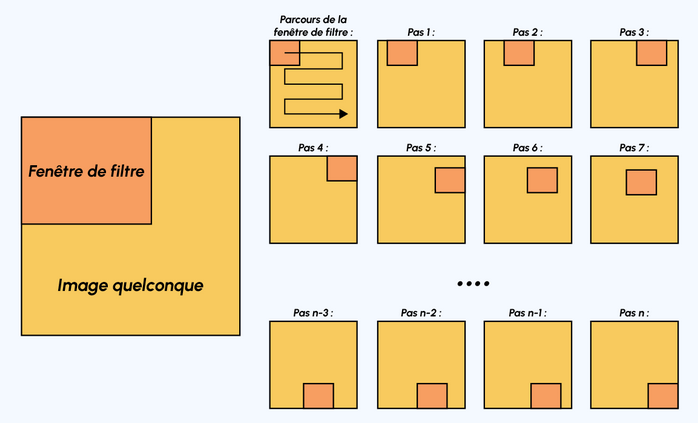
\includegraphics[height=6cm,width=12cm]{Chapitre2/conv.png}
\caption{Principe d'une convolution d'image.}
\label{conv}
\end{figure}

À chaque portion d'image rencontrée, une convolution s'effectue permettant d'obtenir en sortie une \textbf{carte d'activation ou de caractéristiques} ou \textbf{feature map} qui indique où sont localisées les caractéristiques dans l'image. 

\item \underline{\textbf{La couche de pooling:}}
C'est une technique de sous-échantillonnage. Généralement, une couche de pooling est insérée régulièrement entre deux couches convolutives successives.  Cela permet de réduire la taille spatiale des cartes de caractéristiques, donc le nombre de paramètres du réseau, ce qui accélère le temps de calcul et contrôle le risque de sur-apprentissage. 
Les trois types d'opérations de pooling sont :
\begin{itemize}
\item Le max pooling : la valeur de pixel maximale de la partie de l'image couverte par la fenêtre du filtre est renvoyée (voir figure \ref{pool}).
\item Le min pooling : La valeur de pixel minimale  de la partie de l'image couverte par la fenêtre du filtre est renvoyée.
\item Average pooling : la valeur moyenne de tous les pixels  de la partie de l'image couverte par la fenêtre du filtre est renvoyée(voir figure \ref{pool}).
\end{itemize}
 
     \begin{figure}[H]
          \centering
          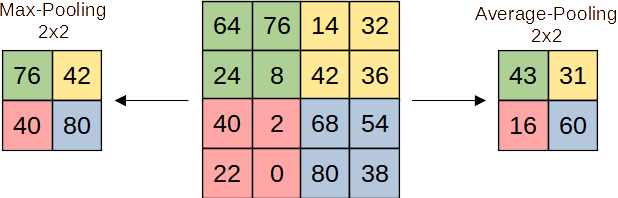
\includegraphics[height=5cm,width=15cm]{Chapitre2/img3.png}
          \caption{Max-pooling et Average-pooling.}
          \label{pool}
          \end{figure}

Les trois opérations de pooling sont illustrées dans la figure \ref{poolef}

\begin{figure}[H]
\centering
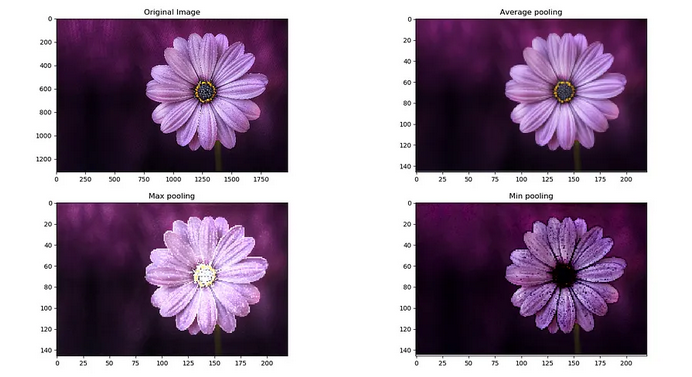
\includegraphics[height=5.5cm,width=11cm]{Chapitre2/poolef.png}
\caption{Average, Max and Min pooling de taille 9 x 9 appliqués à une image.}
\label{poolef}
\end{figure}

\item \underline{\textbf{La couche de correction (ReLu) :}}
La couche de correction est l'application d'une fonction non-linéaire(voir la figure \ref{relu} aux sorties de la couche de convolution, où toutes les valeurs de pixels négatifs sont mises à zéro. Le but est d'introduire la non-linéarité dans le CNN, ce qui permet de faciliter l'extraction des caractéristiques complexes qui ne peuvent pas être modélisées par une combinaison linéaire.

\begin{figure}[H]
\centering
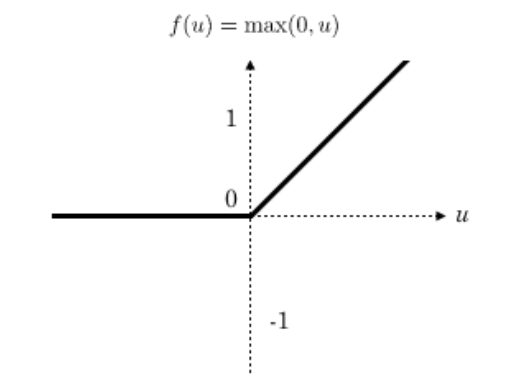
\includegraphics[height=4.5cm,width=6cm]{Chapitre2/relu.png}
\caption{La fonction ReLu.}
\label{relu}
\end{figure}

\item \underline{\textbf{La couche entièrement connectée(FC):}}
La couche entièrement connectée est un perceptron multicouche traditionnel (Multi Layer Perceptron) utilisant une fonction d'activation notamment appelée softmax dans la couche de sortie. 

Elle est entièrement connectée, car chaque neurone dans la couche précédente est connecté à chaque neurone sur la couche suivante. La couche entièrement connectée utilise ses sorties pour classer l'image d'entrée dans différentes classes en fonction de l'ensemble de données d'apprentissage \cite{CNN2015}.  
\end{enumerate}     
     % =========== Fully Connected Layer ===========
La figure \ref{img4} montre un exemple d'une structure d'un réseau de neurones convolutif:
     \begin{figure}[H]
          \centering
          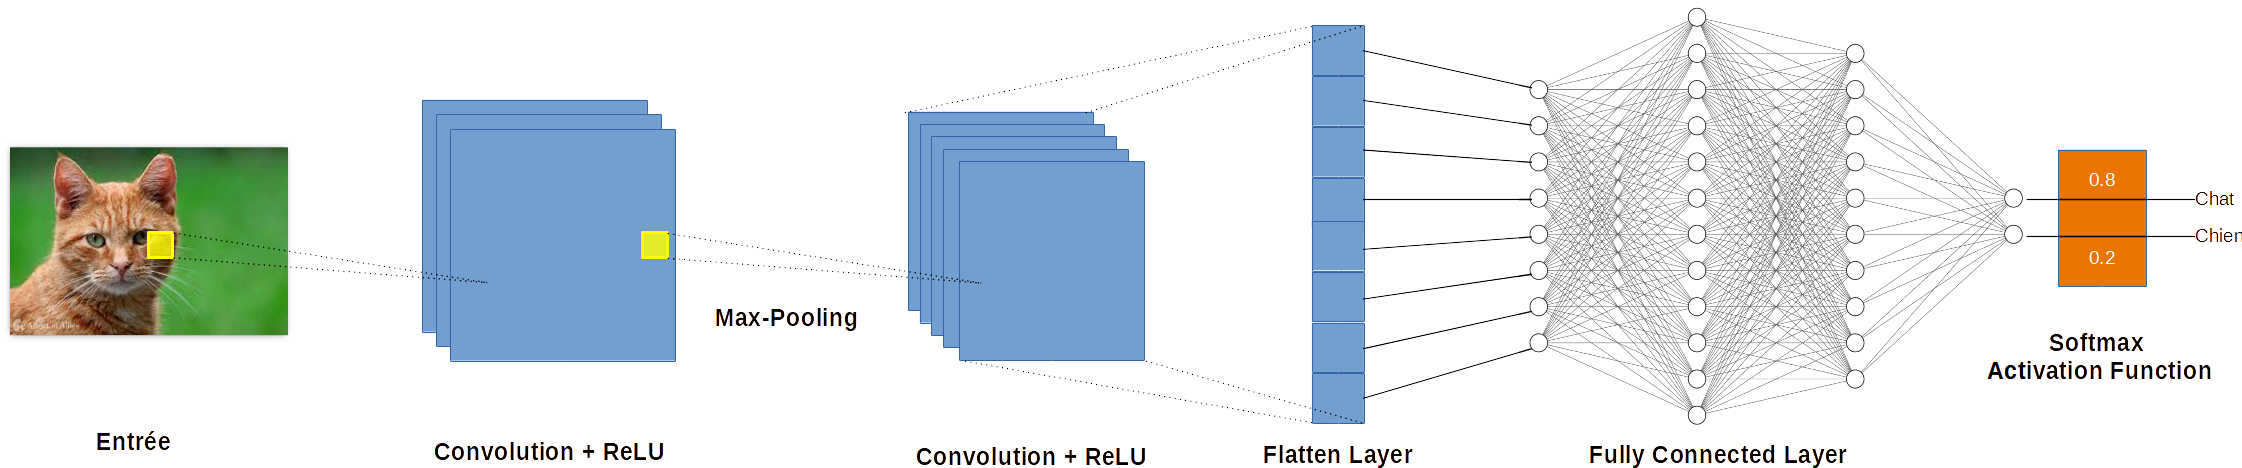
\includegraphics[height=4cm,width=18cm]{Chapitre2/img4.png}
          \caption{Exemple de structure de réseaux de neurones convolutif.}
          \label{img4}
          \end{figure}

% =========== Transfer Learning ===========
     \subsection{L'apprentissage par transfert} 
     L'apprentissage par transfert se produit lorsque des modèles existants sont réutilisés pour résoudre un nouveau défi ou problème. L'apprentissage par transfert n'est pas un type distinct d'algorithme d'apprentissage automatique, mais plutôt une technique ou une méthode utilisée lors de l'entraînement des modèles. Les connaissances acquises lors des entraînements précédents sont recyclées pour aider à effectuer une nouvelle tâche. La nouvelle tâche sera liée d'une certaine manière à la tâche précédemment entraînée.

     Le processus prend des parties pertinentes d'un modèle existant et les applique pour résoudre un problème nouveau mais similaire. Un élément clé de l'apprentissage par transfert est la généralisation. Cela signifie que seules les connaissances pouvant être utilisées par un autre modèle dans différents scénarios ou conditions sont transférées. Au lieu que les modèles soient liés de manière rigide à un ensemble de données d'entraînement, les modèles utilisés dans l'apprentissage par transfert seront plus généralisés. Les modèles développés de cette manière peuvent être utilisés dans des conditions changeantes et avec différents ensembles de données.
     \begin{figure}[H]
          \centering
          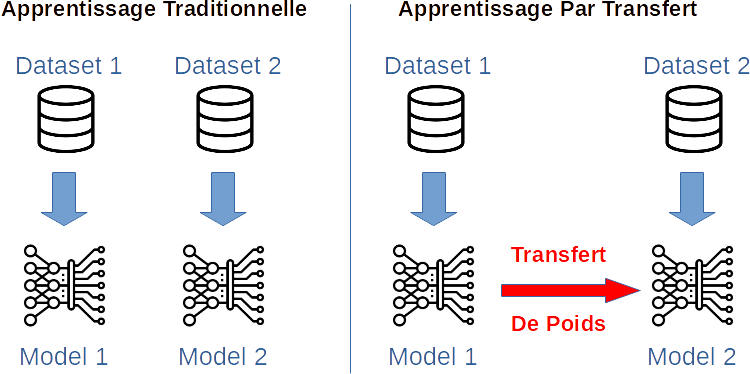
\includegraphics[height=7cm,width=13cm]{Chapitre2/img5.png}
          \caption{Différence entre l'apprentissage traditionnel et l'apprentissage par transfert.}
          \label{img5}
          \end{figure}

% =========== Backbones =========== 
\section{Architectures de réseau profond populaires} 
Certains réseaux profonds ont apporté des contributions si importantes dans le domaine qu'ils sont devenus des normes largement connues. C'est le cas d'AlexNet, VGG-16, GoogLeNet et ResNet. Leur importance était telle qu'ils sont actuellement utilisés comme éléments de base pour de nombreuses architectures de détection d'objets. Pour cette raison, nous consacrerons cette section à leur présentation. 

\begin{enumerate}
\item \textbf{AlexNet}\cite{alexnet}\\
AlexNet a été le  CNN pionnier qui a largement surpassé ses concurrents au défi ImageNet ILSVRC-2012 avec une précision de test TOP-5 de 84,6\% tandis que le concurrent le plus proche, qui utilisait des techniques traditionnelles au lieu d'architectures profondes, a atteint une précision de 73,8\% dans le même défi. L'architecture présentée par Krizhevsky et coll. était relativement simple, elle est composée de huit couches d'entraînement, cinq couches de convolution et trois couches entièrement connectées. Toutes les couches entraînables sont suivies d'une fonction d'activation (ReLu) à l'exception de la dernière couche entièrement connectée où une fonction softmax est utilisée. L'architecture aussi se compose de couches
non entraînables : trois couches de pooling, deux couches de normalisation et une couche Dropout. cette architecture est clairement présentée sur la figure\ref{alexnet}.

\begin{figure}[H]
\centering
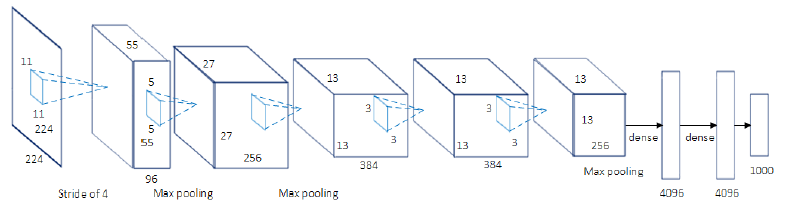
\includegraphics[height=2in,width=6in]{Chapitre2/alexnet.png}
\caption{Architecture du réseau convolutif AlexNet. \cite{alexnet}}
\label{alexnet}
\end{figure} 
\item \textbf{VGG}\cite{vgg}\\
Visual Geometry Group (VGG) est un modèle CNN introduit par le Groupe de Géométrie Visuelle (VGG) de l'Université d'Oxford. Ils ont proposé divers modèles et configurations de CNN profonds, l'un d'eux a été soumis au ImageNet Large Scale Visual Recognition Challenge (ILSVRC)-2013. Ce modèle, également connu sous le nom de VGG-16 , est devenu populaire grâce à sa précision  de test TOP-5 de 92,7\% . 
La figure \ref{vgg} montre la configuration de VGG-16. La principale différence entre VGG - 16 et ses prédécesseurs est l'utilisation d'un empilement de couches de convolution avec de petits champs réceptifs  dans les premières couches au lieu de quelques couches avec grands champs réceptifs. Cela conduit à moins de paramètres et plus de non-linéarités entre les deux, rendant ainsi la fonction de décision plus discriminante et le modèle plus facile à entraîner.
\begin{figure}[H]
\centering
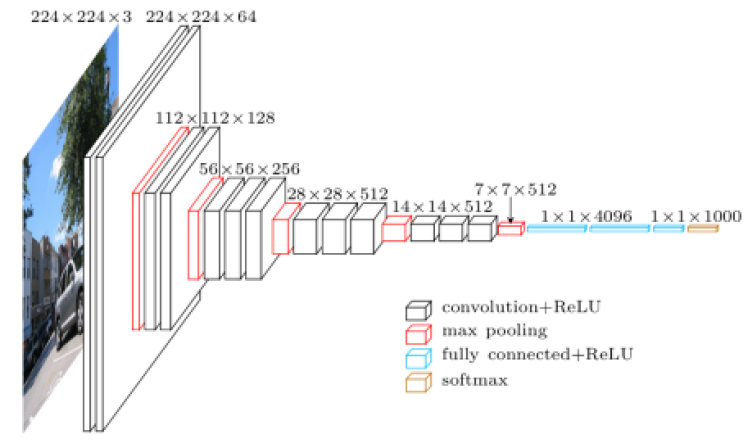
\includegraphics[height=2in,width=6in]{Chapitre2/vgg.png}
\caption{Architecture du réseau convolutif VGG-16. }
\label{vgg}
\end{figure} 
\item \textbf{GoogleNet}\cite{google}\\
En 2014, les chercheurs de Google ont présenté le réseau GoogLeNet, qui a pris la première place du concours ImageNet en 2014 pour les défis de classification et de détection. La principale caractéristique intéressante de GoogLeNet est qu'il fonctionne très rapidement en raison de l'introduction d'un nouveau concept appelé (inception module), il est clairement illustré sur la figure \ref{google}. Ce module est basé sur plusieurs très petites convolutions afin de réduire drastiquement le nombre de paramètres à seulement 5 millions ; c'est 12 fois moins qu'AlexNet. Il utilise moins de mémoire et moins d'énergie. L'architecture GoogLeNet se compose de 22 couches.GoogLeNet est principalement utilisé dans le modèle de détection d'objets YOLO.
\begin{figure}[H]
 \centering
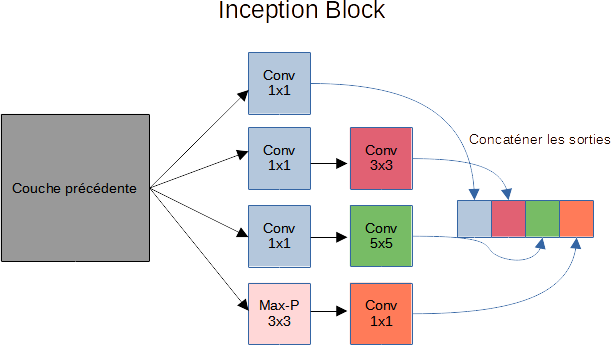
\includegraphics[height=8cm,width=12cm]{Chapitre2/img9.png}
\caption{Structure de Inception Block.}
 \label{img9}
 \end{figure}

\item \textbf{ResNet}\cite{resnet}\\
Les réseaux résiduels profonds (ResNet) sont basés sur l'idée de développer des réseaux beaucoup plus profonds (des centaines de couches par opposition à des dizaines de couches). Dans ResNets, les couches de convolution sont divisées en blocs résiduels (voir figure \ref{resnet}), et pour chaque bloc, une connexion résiduelle est ajoutée, qui contourne le bloc correspondant. Ensuite, la sortie du bloc résiduel est additionnée avec l'entrée d'origine passée à travers la connexion résiduelle. 
\begin{figure}[H]
\centering
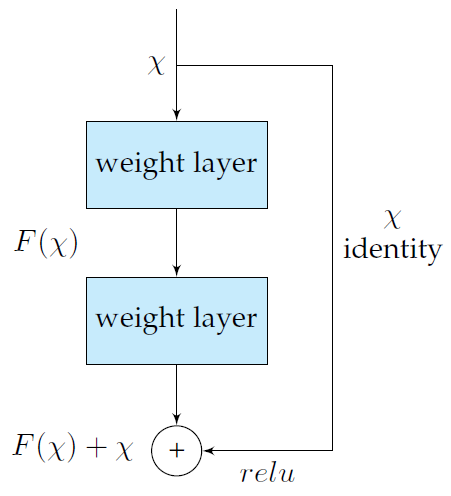
\includegraphics[height=2in,width=2.5in]{Chapitre2/resnet.png}
\caption{ Bloc résiduel de l'architecture ResNet. \cite{resnet}}
\label{resnet}
\end{figure} 

\item \textbf{SqueezeNet} \cite{SqueezeNet2016}
Une petite architecture CNN avec une précision équivalente à AlexNet. Ça peut être  3 fois plus rapide et 500 fois plus petit qu'AlexNet.
Il est construit sur une architecture spécifique, que l'on appelle (Fire module) qui contient une couche de compression(Squeeze) et une couche d'extension (expand), il est clairement illustré sur la figure \ref{SN}.

Les couches de compression(Squeeze) sont des couches de convolution composées uniquement de filtres $1\times 1$ et les couches d'extension sont des couches de convolution avec un mélange de filtres $1 \times 1$ et $3 \times 3$.
\begin{figure}[H]
\centering
  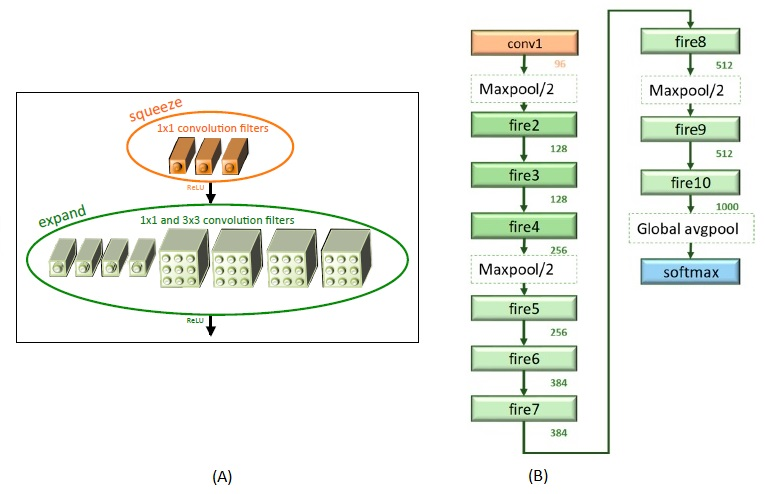
\includegraphics[width=9cm, height=7cm]{Chapitre2/SN.jpg} 
   \caption{(A) Fire module (B)Architecture de SqueezeNet \cite{SqueezeNet2016}.}
   \label{SN}
 \end{figure}

\item \textbf{ShuffleNet} \cite{shufflenet2018} et \textbf{ShuffleNetV2}\cite{shufflenetV2}
Une architecture CNN très efficace en termes de calcul, conçue principalement pour les appareils mobiles avec une puissance de calcul limitée. L'architecture introduit deux opérations clés pour réduire considérablement les coûts de calcul tout en conservant la précision. La première opération consiste en des convolutions de groupe par points (pointwise group convolutions), qui peuvent réduire la complexité de calcul des convolutions 1 × 1. Néanmoins, ces convolutions ont un effet secondaire, qui fait que les outputs d'un canal en particulier ne sont dérivées que d'une petite fraction des canaux d'input. Cet effet peut être diminué en divisant les canaux de chaque groupe en de multiples sous-groupes, ce qui est l'opération de mélange de canaux (channel shuffle).

ShuffleNetV2 propose de nombreux guides pratiques pour des architectures CNN efficientes. Il optimise davantage l’architecture avec des changements dans le goulot d’étranglement et en présentant la division de canaux (channel split). La figure montre clairement les différences entre ShuffleNet (a., b.) et ShuffleNetV2 (c. d.).

\begin{figure}[H]
\centering
  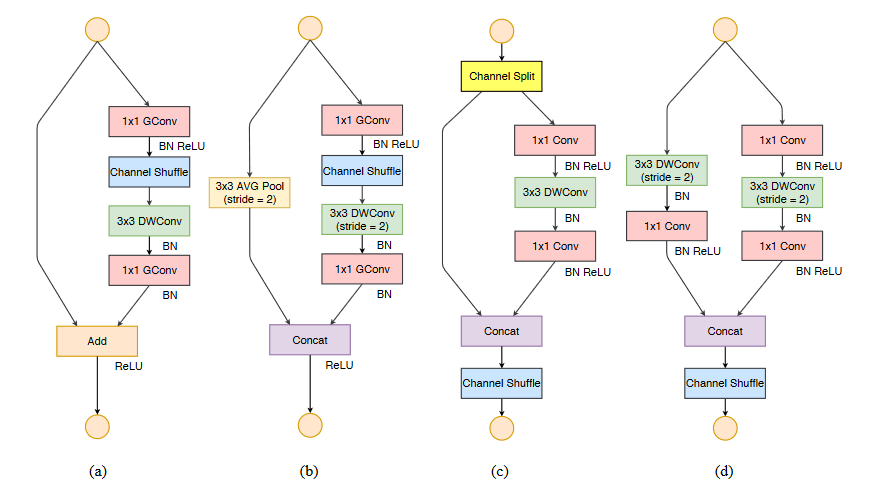
\includegraphics[width=17cm, height=7cm]{Chapitre2/shuffle.png} 
   \caption{Les unités de construction de l'architecture ShuffleNet  \cite{shufflenet2018} et ShuffleNetV2\cite{shufflenetV2}.}
   \label{shuffle}
 \end{figure}
 
\item \textbf{MobileNetV2 } \cite{mobilenetv2}
La version deux des séries MobileNet introduit les résiduels inversés (inverted residuals) et les goulots d'étranglement linéaires (linear bottlenecks) pour améliorer les performances de MobileNets. Les résiduels inversés permettent au réseau de calculer des activations (ReLU) de manière plus efficace, et de maintenir plus d’informations après activation. La figure \ref{mobv2} montre le goulot d'étranglement, et inclue les résiduels inversés. Sur ce schéma, les blocs plus épais ont plus de canaux. 

\begin{figure}[H]
\centering
  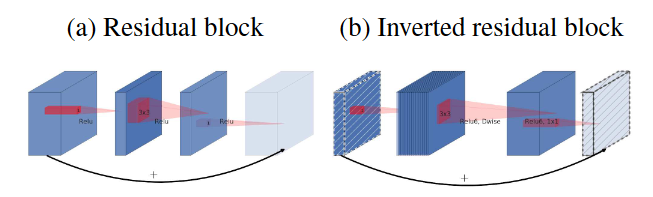
\includegraphics[width=10cm, height=5cm]{Chapitre2/mobv2.png} 
   \caption{La différence entre bloc résiduel \cite{mobilenet}
et résiduel inversé \cite{mobilenetv2}.}
   \label{mobv2}
 \end{figure}
 
\item \textbf{Darknet-53} \cite{yolov3_paper}
Introduit en 2018 Darknet-53 par Joseph Redmon Ali Farhadi, c'est un réseau neuronal convolutif qui sert de base pour l'extraction de caractéristiques dans l'approche de détection d'objets YOLOv3. C'est une amélioration de son prédécesseur Darknet-19 sur lequel est basé l'architecture de YOLOv2.
Les améliorations par rapport à Darknet-19 incluent l'utilisation de connexions résiduelles, ainsi que davantage de couches.

L'architecture du réseau Darknet-53 est illustrée à la figure \ref{img10}. Ce modèle de réseau combine les blocs résiduels et le réseau d'extraction de caractéristiques de base YOLOv2, Darknet-19 \cite{yolov3_paper}, en utilisant des couches de convolution et des blocs résiduels successifs $1\times 1$ et $3\times 3$. La couche convolutive, la couche de normalisation par lots et la couche Leaky Relu constituent ensemble sa plus petite composante.

           \begin{figure}[H]
                \centering
                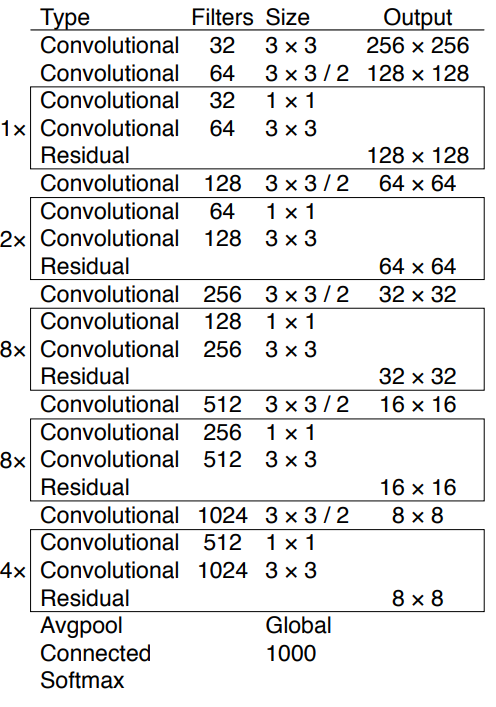
\includegraphics[height=9cm,width=8cm]{Chapitre2/img10.png}
                \caption{Architecture du réseau Darknet-53 \cite{yolov3_paper}.}
                \label{img10}
                \end{figure}

Notez que le classificateur en bas n'est utilisé que lors de l'utilisation du réseau pour la classification d'objets plutôt que pour la localisation d'objets. 

\end{enumerate}


     
          % =========== AlexNet =========== 

          % =========== VGG-16 ===========


          % =========== ResNet ===========
          
          % =========== GoogLeNet ===========

           % =========== Darknet-53 ===========





\section{Les méthodes de détections d'objets basées sur l'apprentissage profond}
Comme nous avons déjà mentionné dans le chapitre précédent, la détection d'objets basée sur l'apprentissage profond est regroupée en deux classes : la "détection en deux étapes" et la "détection en une étape".

En général, les détecteurs d'objets basés sur l'apprentissage en profondeur extraient des caractéristiques de l'image d'entrée. Un détecteur d'objets résout deux tâches successives :
\begin{itemize}
\item  Tâche n° 1 : trouver un nombre arbitraire d'objets (peut-être même zéro), et
\item  Tâche n° 2 : classer chaque objet et estimer sa taille à l'aide d'un cadre englobant.
\end{itemize}

Pour simplifier le processus, on peut séparer ces tâches en deux étapes. D'autres méthodes combinent les deux tâches en une seule étape (détecteurs à une étape) pour obtenir des performances plus élevées au détriment de la précision.

% =========== Two-Stage ===========
\subsection{La détection d'objets en deux étapes}
 
Dans les détecteurs d'objets à deux étages, les régions d'objet approximatives sont proposées à l'aide de caractéristiques profondes avant que ces caractéristiques ne soient utilisées pour la classification.

     L'architecture en deux étapes implique une proposition de région d'objet avec des méthodes conventionnelles de vision par ordinateur ou des réseaux profonds, suivie d'une classification d'objet basée sur des caractéristiques extraites de la région proposée.   
     Ces méthodes permettent d'obtenir une précision de détection  plus élevée, mais sont généralement plus lentes. 
     
    
     % =========== RCNN ===========
\subsubsection{Les modèles R-CNN}  
La famille de méthodes R-CNN fait référence au R-CNN, qui peut signifier "Régions avec des caractéristiques CNN" ou "Réseau de neurones convolutifs basés sur les régions", développé par Ross Girshick, et al.

Cela inclut les techniques R-CNN, Fast R-CNN et Faster-RCNN conçues et démontrées pour la localisation et la reconnaissance d'objets.

\begin{enumerate}
 \item  \textbf{R-CNN}\cite{rcnn_paper}
 
Le R-CNN a été introduit par Ross Girshick et al en 2004. Il s'agit peut-être de l'une des premières applications importantes des réseaux de neurones convolutifs au problème de la localisation, de la détection et de la segmentation d'objets. Le modèle R-CNN proposé est composé de trois modules qui sont:
\begin{itemize}
\item \underline{Module 1 : Proposition de Région.} Générez et extrayez des propositions de régions indépendantes des catégories, par ex. boîtes englobantes candidates.
\item \underline{Module 2 : Extracteur de caractéristiques.} Extraire une caractéristique de chaque région candidate, par ex. à l'aide d'un réseau de neurones à convolution profonde.
\item \underline{Module 3 : Classificateur.} Classer les caractéristiques comme faisant partie de la classe connue, par ex. modèle de classificateur SVM linéaire.
\end{itemize}
 
L'architecture du modèle est résumée dans l'image ci-dessous.
 \begin{figure}[H]
          \centering
          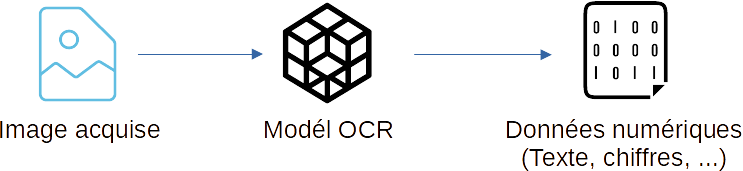
\includegraphics[height=6cm,width=15cm]{Chapitre2/img11.png}
          \caption{Architecture d'un R-CNN \cite{rcnn_paper}}
          \label{img11}
          \end{figure}

Une Recherche sélective qui est une technique de vision par ordinateur est utilisée pour proposer des régions candidates ou des boîtes englobantes d'objets potentiels dans l'image, bien que la flexibilité de la conception permette d'utiliser d'autres algorithmes de proposition de région.

L'extracteur de caractéristiques utilisé par le modèle est le modèle AlexNet. La sortie du CNN est un vecteur de 4 096 éléments qui décrit le contenu de l'image. Ce dernier est transmis à un SVM linéaire pour la classification, en particulier un SVM est entraîné pour chaque classe connue.

Il s'agit d'une application relativement simple et directe des CNN au problème de la localisation et de la reconnaissance d'objets. Un inconvénient de l'approche est qu'elle est lente, nécessitant une phase d'extraction de caractéristiques basée sur un CNN sur chacune des régions candidates générées par l'algorithme de proposition de région. C'est un vrai problème car le document initiale décrit le modèle fonctionnant sur environ 2 000 régions proposées par image au moment du test.
          
 \item  \textbf{Fast R-CNN}\cite{fast_rcnn_paper}
 
Fast R-CNN a été proposé par Ross Girshick en 2015 comme extension aux R-CNN  pour résoudre les problèmes de vitesse.

Fast R-CNN est proposé comme un modèle unique au lieu d'un pipeline pour apprendre et produire directement des régions et des classifications.

L'architecture du modèle prend l'image comme entrée d'un ensemble de propositions de régions qui sont transmises à travers un réseau de neurones convolutif. Un CNN pré-entraîné, tel qu'un VGG-16, est utilisé pour l'extraction de caractéristiques. La sortie du CNN est une couche personnalisée appelée couche de regroupement de régions d'intérêt, ou regroupement RoI (Region of Interest Pooling Layer, or RoI Pooling), qui extrait des caractéristiques spécifiques à une région candidate d'entrée donnée. 

La sortie du CNN est ensuite interprétée par une couche entièrement connectée, puis le modèle se divise en deux sorties, une pour la prédiction de classe via une couche softmax, et une autre avec une sortie linéaire pour la boîte englobante. Ce processus est ensuite répété plusieurs fois pour chaque région d'intérêt dans une image donnée.

L'architecture du modèle est résumée dans l'image \ref{img13}

\begin{figure}[H]
          \centering
          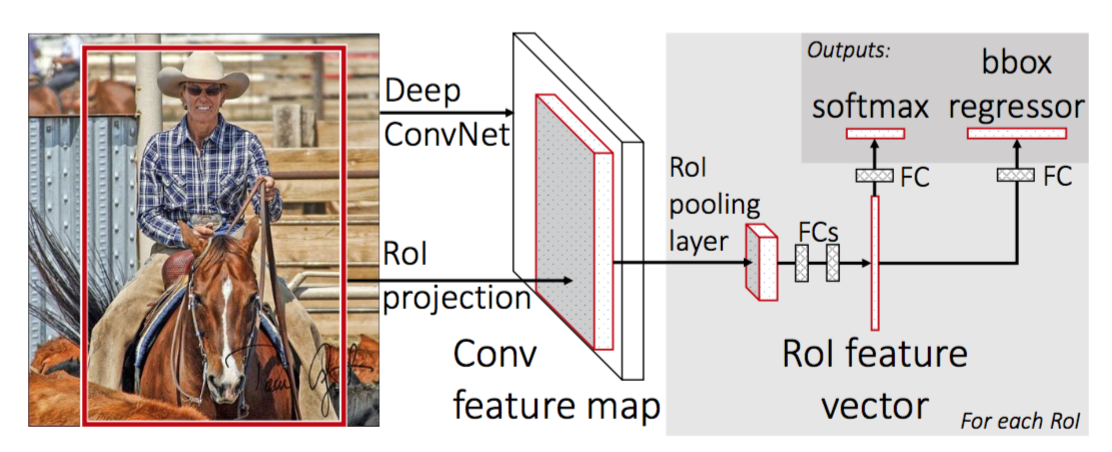
\includegraphics[height=5cm,width=15cm]{Chapitre2/img13.png}
          \caption{Architecture d'un Fast-RCNN \cite{fast_rcnn_paper}}
          \label{img13}
          \end{figure}

Le modèle est beaucoup plus rapide à entraîner et à faire des prédictions, mais nécessite toujours qu'un ensemble de régions candidates soit proposé avec chaque image d'entrée.

 \item  \textbf{Faster R-CNN}\cite{faster_rcnn_paper}
 
Proposée par Shaoqing Ren, et al. en 2016, toujours dans le but d'améliorer la vitesse d'entraînement et de détection des modèles précédemment décrits.

L'architecture a été conçue à la fois pour proposer et affiner les propositions de région dans le cadre du processus d'entraînement, appelé Réseau de proposition de régions, ou RPN. Ces régions sont ensuite utilisées parallèlement avec un modèle Fast R-CNN dans une conception de modèle unique. Ces améliorations réduisent à la fois le nombre de propositions de régions et accélèrent le fonctionnement en temps de test du modèle.

Bien qu'il s'agit d'un seul modèle unifié, l'architecture est composée de deux modules :
\begin{itemize}
\item \underline{Module 1 : Réseau de proposition de région.}  Réseau de neurones convolutifs pour proposer des régions et le type d'objet à considérer dans la région.
\item \underline{Module 2 : R-CNN rapide.} Réseau neuronal convolutif pour extraire les caractéristiques des régions proposées et produire la boîte englobante et les étiquettes de classe.
\end{itemize}

Les deux modules fonctionnent sur la même sortie d'un CNN profond. Le réseau de proposition de région agit comme un mécanisme d'attention pour le réseau Fast R-CNN, informant le deuxième réseau de l'endroit où regarder ou prêter attention.

L'architecture du modèle est résumée dans l'image \ref{img14}:

\begin{figure}[H]
          \centering
          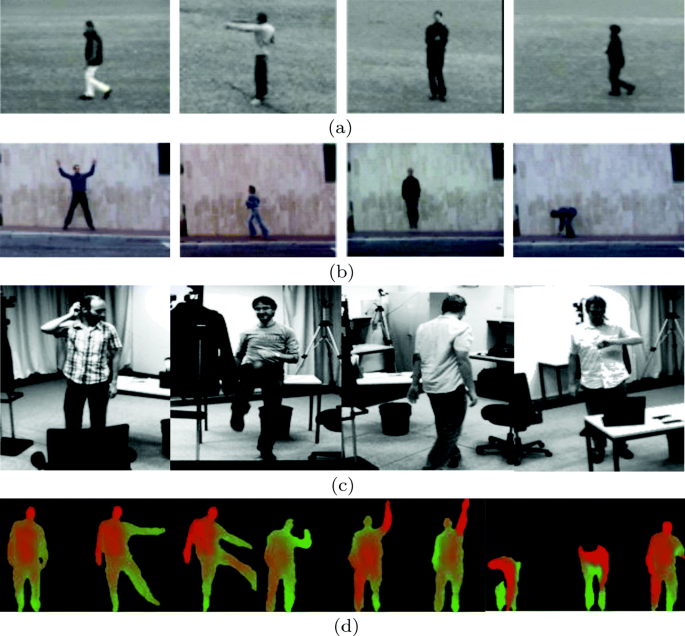
\includegraphics[height=13cm,width=8cm]{Chapitre2/img14.png}
          \caption{Architecture d'un Faster-RCNN}
          \label{img14}
          \end{figure}
          
Le RPN fonctionne en prenant la sortie d'un CNN profond pré-entraîné, tel que VGG-16, et en passant un petit réseau sur la carte des caractéristiques et en produisant plusieurs propositions de régions et une prédiction de classe pour chacune. Les propositions de régions sont des boîtes englobantes, basées sur des boîtes dites d'ancrage ou des formes prédéfinies conçues pour accélérer et améliorer la proposition de régions. La prédiction de classe est binaire, indiquant la présence d'un objet, ou non.

Une procédure d'apprentissage alterné est utilisée où les deux sous-réseaux sont entraînés en même temps. Cela permet aux paramètres du CNN profond du détecteur de caractéristiques d'être adaptés ou affinés pour les deux tâches en même temps.
 \end{enumerate} 


     % =========== Fast-RCNN ===========
    
     % =========== Faster-RCNN ===========
     
% =========== One-Stage ===========
\subsection{La détection d'objets en une étape}
Contrairement aux détecteurs à deux étapes, ces modèles ignorent l'étape de proposition de région des modèles à deux étages et exécutent la détection directement sur un échantillonnage dense d'emplacements. Ils considèrent généralement toutes les positions sur l'image comme des objets potentiels et essaient de classer chaque région d'intérêt comme arrière-plan ou comme objet cible.

     % =========== YOLO ===========
\subsubsection{YOLO (You Only Look Once) \cite{yolo_paper} }

Le modèle a été décrit pour la première fois par Joseph Redmon et al. en 2015. 
L'approche implique un seul réseau neuronal entraîné de bout en bout qui prend une image en entrée et prédit directement les boîtes englobantes et les étiquettes de classe pour chaque boîte englobante. La technique offre une précision prédictive inférieure (par exemple, plus d'erreurs de localisation), bien qu'elle fonctionne à 45 images par seconde et jusqu'à 155 images par seconde pour une version optimisée en vitesse du modèle.

En outre, YOLO sélectionne GoogLeNet comme réseau de base. Il se compose de 24 couches convolutives et de 2 couches entièrement connectées avec une entrée réseau de 448 × 448 images. Il divise l'image complète en grilles S×S. Chaque cellule de grille est responsable de la détection du centre de l'objet tombant dans la cellule de grille. Chaque cellule de la grille prédit les probabilités de classe C, les boîtes englobantes B et les scores de confiance, et l'image complète est codée pour produire le tenseur SxSx(5B+C).
     \begin{figure}[H]
          \centering
          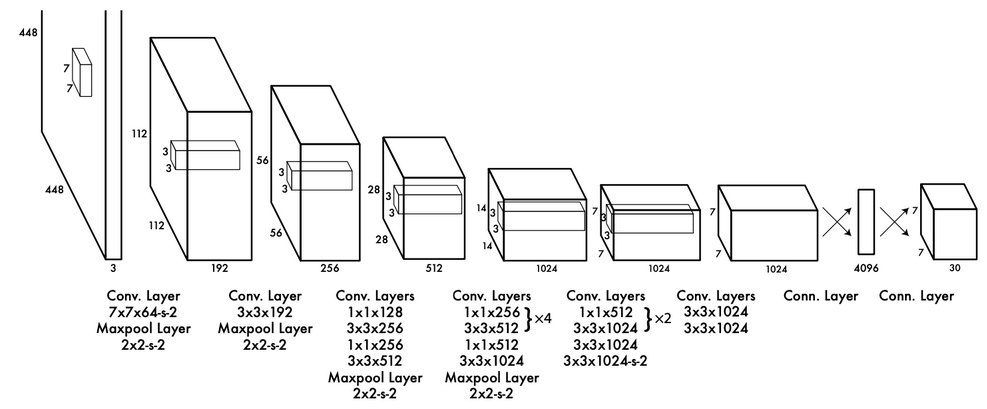
\includegraphics[height=7cm,width=16cm]{Chapitre2/img151.png}
          \caption{Architecture de YOLO (You Only Look Once)}
          \label{img15}
          \end{figure}

     % =========== YOLOv3 ===========
\subsubsection{YOLOv3 \cite{yolov3_paper}} 

Proposé par Redmon J et Farhadi deux ans plus tard en 2018 après la première version de YOLO. c'est une version améliorée de YOLO et YOLOv2. Il existe des différences majeures entre YOLOv3 et les anciennes versions en termes de vitesse, de précision et de spécificité des classes. YOLOv2 utilise Darknet-19 comme extracteur de caractéristiques de base, tandis que YOLOv3 utilise Darknet-53.    
    
Darknet-53  combine des blocs résiduels et FPN (Feature Pyramid Network). C'est un extracteur de caractéristiques qui prend une image à échelle unique d'une taille arbitraire en entrée et des sorties proportionnellement dimensionnées cartes de fonctionnalités à plusieurs niveaux, ce qui donne de bonnes performances sur une large gamme de résolutions d'entrée.

Darknet-53  est plus puissant que le Darknet-19 et plus efficace que les backbones concurrents (ResNet-101 ou ResNet-152). Il est également rapide et précis en termes de précision moyenne moyenne (mAP) et de valeurs d'intersection sur l'union (IOU). Il fonctionne beaucoup plus rapidement que les autres méthodes de détection avec des performances comparables.

     \begin{figure}[H]
          \centering
          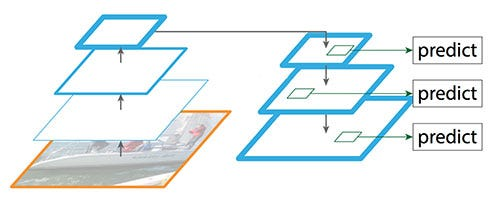
\includegraphics[height=5cm,width=9cm]{Chapitre2/img16_.jpg}
          \caption{Feature Network Pyramid (FNP)}
          \label{img16_}
          \end{figure}
     \begin{figure}[H]
          \centering
          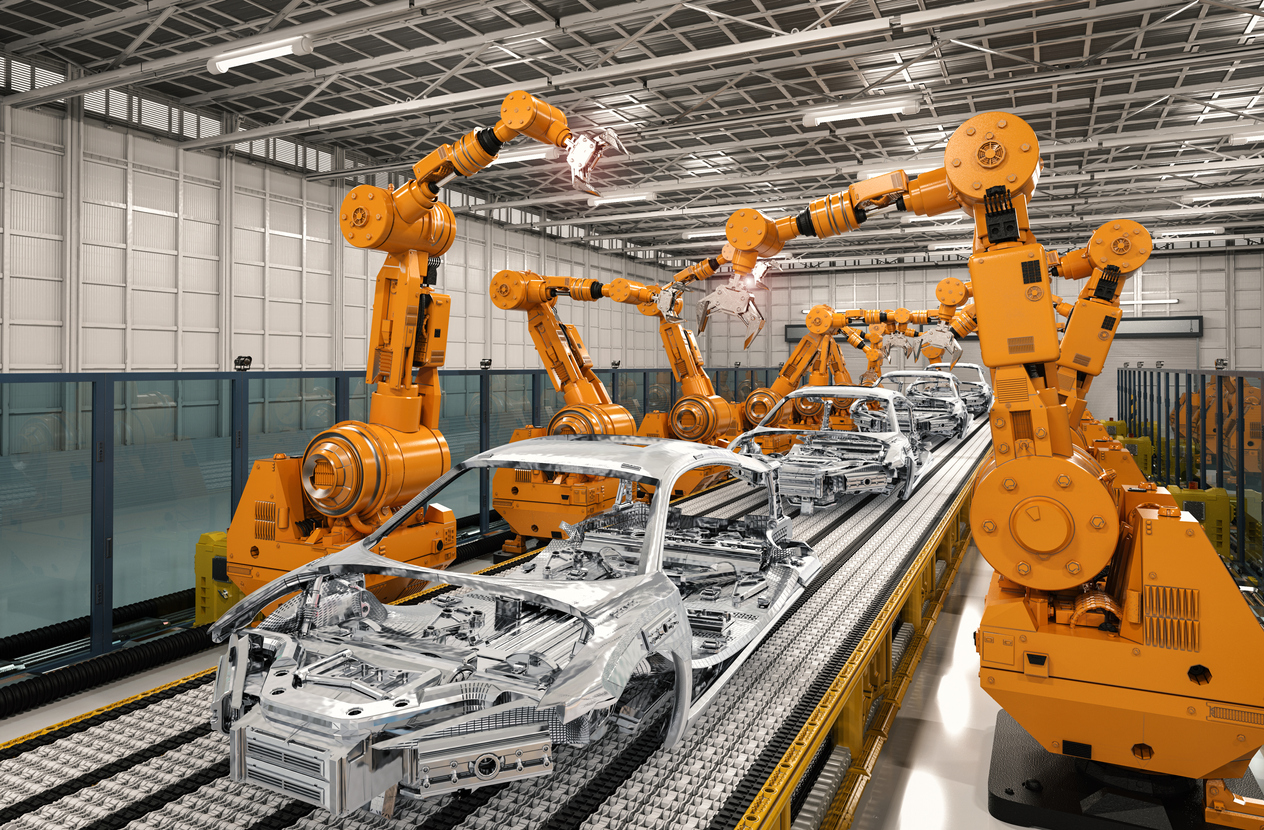
\includegraphics[height=6cm,width=14cm]{Chapitre2/img16.jpg}
          \caption{Architecture de YOLOv3}
          \label{img16}
          \end{figure}
     

\subsubsection{YOLOv4\cite{yolov4_paper} }

Créé par Alexeï Bochkovski en 2020, L'architecture de YOLOv4 est composée de CSPDarknet53 en tant que pilier, ce pilier est basé sur DarkNet-53 et utiliser une stratégie CSPNet\cite{cspnet} pour diviser la carte des caractéristiques de la couche de base en deux parties, puis les fusionne via une hiérarchie à plusieurs étapes. L'utilisation d'une stratégie de division et de fusion permet un flux plus dégradé à travers le réseau.

Après le pilier, PANet\cite{panet} est utilisé comme méthode d'agrégation de paramètres à partir de différents niveaux de pilier pour différents niveaux de détecteur, au lieu du FPN utilisé dans YOLOv3.

De plus, le bloc SPP\cite{spp} est également ajouté car il augmente considérablement le champ de réception, sépare les caractéristiques de contexte les plus importantes et ne provoque pratiquement aucune réduction de la vitesse de fonctionnement du réseau.
enfin, YOLOv3 est utilisé comme la tête de réseaux.
\begin{figure}[H]
          \centering
          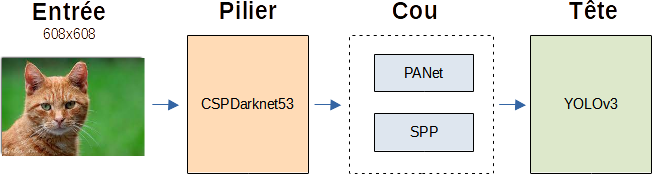
\includegraphics[height=4cm,width=16cm]{Chapitre2/arch_yolov4.png}
          \caption{Architecture de YOLOv4.}
          \label{img16_}
          \end{figure}

\subsubsection{YOLOv5} 
Développé par ultralytics en 2020, il a été une énorme amélioration de l'accessibilité pour la détection d'objets en temps réel en raison de la transition de Darknet à PyTorck en tant que cadre de mise en œuvre, car Darknet est plus difficile à configurer et moins prêt pour la production. Cette transition a entraîné une forte augmentation du temps de formation et également du temps de prédiction avec l'accessibilité au grand écosystème de PyTorch.          

L'architecture de ce modèle est similaire à YOLOv4 mais CSPDarknet53 comme pilier, SPP et PANet pour le cou et YOLOv3 comme tête. La principale différence avec les techniques d'augmentation de données comme l'augmentation de mosaïque où plusieurs images sont combinées pour former une image unique avec différents contextes, cette technique apprend au modèle à reconnaître des objets dans différentes localisations sans trop s'appuyer sur un contexte spécifique. Cela améliore les performances du modèle en rendant l'algorithme plus robuste à l'environnement des objets.
\begin{figure}[H]
          \centering
          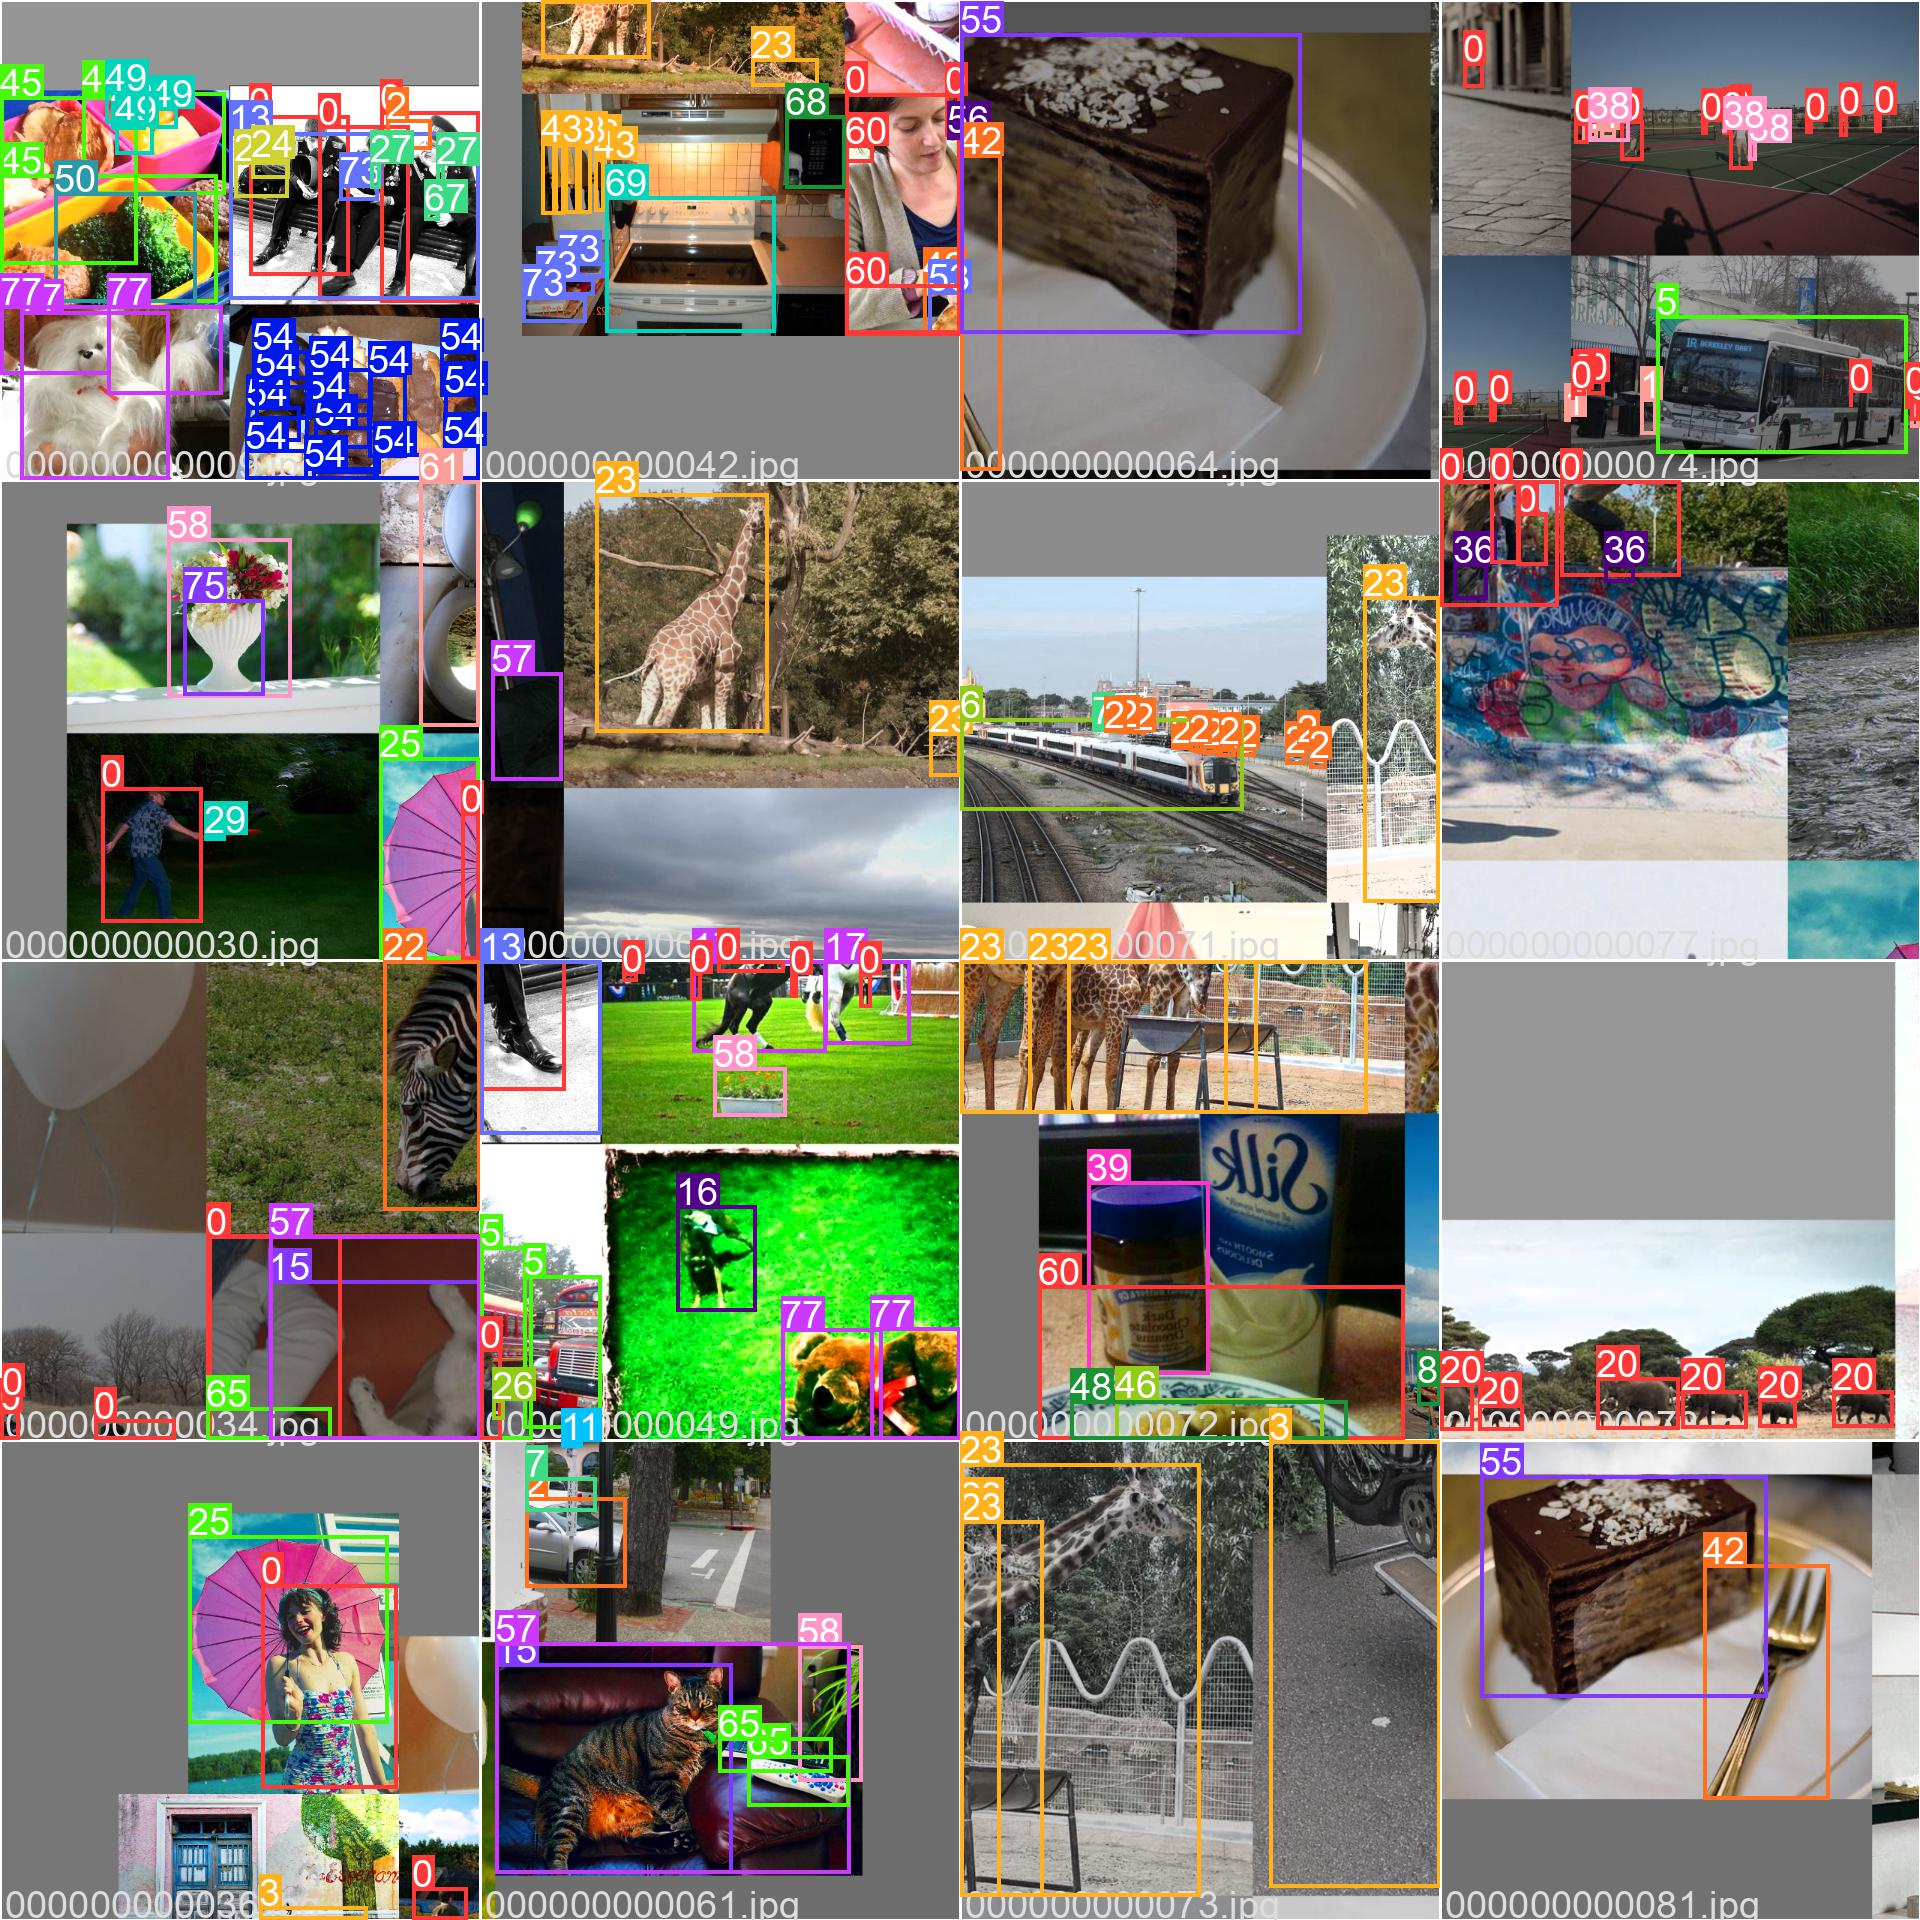
\includegraphics[height=9cm,width=14cm]{Chapitre2/yolov5_data.jpg}
          \caption{Résultat de la technique d'augmentation de données Mosaic.}
          \label{yolov5_mosa}
          \end{figure}

% =========== SSD ===========
% =========== Evaluation Metrics ===========
\section{Métriques pour l'évaluation des systèmes de détection d'objets} 
Pour qu'un système de détection d'objets soit utile et ait le potentiel d'apporter une contribution significative sur le terrain, son efficacité doit être soigneusement évaluée. En outre, l'évaluation doit être effectuée à l'aide de critères généraux et connus permettant une comparaison équitable avec les méthodes existantes et une confirmation de la validité et de l'utilité du système.

Les métriques de détection d'objets servent de mesure pour évaluer les performances du modèle sur une tâche de détection d'objets. Cela nous permet également de comparer objectivement plusieurs systèmes de détection ou de les comparer à une référence. En conséquence, des compétitions importantes telles que PASCAL VOC et MSCOCO fournissent des mesures prédéfinies pour évaluer les performances de différents algorithmes de détection d'objets sur leurs ensembles de données. Dans cette section, nous expliquons les principales métriques de détection d'objets et leur interprétation.
          % =========== IoU ===========
\subsection{Intersection over Union (IoU)}
Étant donné que la tâche de classification évalue uniquement la probabilité que l'objet de classe apparaisse dans l'image, c'est une tâche simple pour un classificateur d'identifier les prédictions correctes des incorrectes. Cependant, la tâche de détection d'objet localise davantage l'objet avec une boîte englobante associée à son score de confiance correspondant pour signaler la certitude avec laquelle la boîte englobante de la classe d'objets a été détectée.

L'intersection over Union, également appelée indice de Jaccard, est une métrique d'évaluation qui quantifie la similarité entre la boîte englobante de vérité terrain  et la boîte englobante prédite pour évaluer la qualité de la boîte prédite. 

Formellement, l'IoU égale à l'intersection entre la boîte de vérité terrain et la boîte prédite sur leur union. La figure \ref{img19} montre clairement cette notion d'IoU
          \begin{figure}[H]
               \centering
               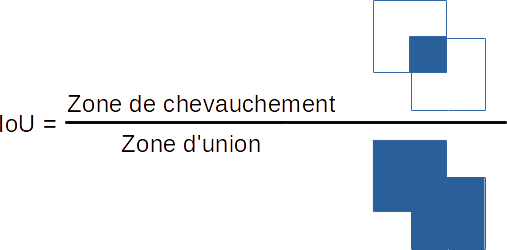
\includegraphics[height=5cm,width=10cm]{Chapitre2/img19.png}
               \caption{Intersection over Union (IoU)}
               \label{img19}
               \end{figure}

Le score IoU varie de 0 à 1, plus les deux boites englobantes sont proches, plus le score IoU est élevé (voir figure \ref{img20}.
          \begin{figure}[H]
               \centering
               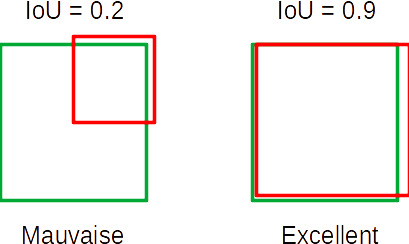
\includegraphics[height=4.5cm,width=8cm]{Chapitre2/img20.png}
               \caption{Exemples de la mesure Intersection over Union (IoU)}
               \label{img20}
               \end{figure}

          % =========== Confusion Matrix ===========
\subsection{Matrice de confusion}

En Choisissant un seuil prédéfini pour la valeur IoU, nous pouvons créer la matrice de confusion qui définit les performances d'un modèle en nous permettant de calculer d'autres mesures comme le rappel et la précision.
          \paragraph{Vrai positif (TP):} IoU >= seuil, une détection correcte. 
          \paragraph{Faux positif (FP):} IoU < seuil, une mauvaise détection.
          \paragraph{Faux négatif (FN):} Le modèle n'a pas détecté l'objet actuel.
          \paragraph{Vrai négatif (TN):} Non utilisé, il représenterait une erreur de détection corrigée. Dans la tâche de détection d'objet, il existe de nombreuses boîtes englobantes possibles qui ne doivent pas être détectées dans une image. Ainsi, TN serait toutes les boîtes englobantes possibles qui n'ont pas été correctement détectées (autant de boîtes possibles dans une image). C'est pourquoi il n'est pas utilisé par les métriques.
          \begin{figure}[H]
               \centering
               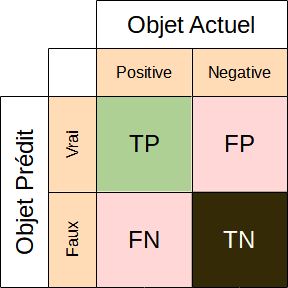
\includegraphics[height=9cm,width=9cm]{Chapitre2/mat_conf.png}
               \caption{Matrice de confusion.}
               \label{mat_conf}
               \end{figure}
          
          % =========== Precision ===========
          \subsection{Précision}
          La précision est la capacité d'un modèle à identifier uniquement les objets pertinents. C'est le pourcentage de prédictions positives correctes et est donné par :
          \begin{center} $Précision = \frac{TP}{TP + FP}$ \end{center}

          % =========== Recall ===========
          \subsection{Rappel}
          Le rappel est la capacité d'un modèle à trouver tous les cas pertinents (toutes les boîtes englobantes souhaitées). C'est le pourcentage de vrais positifs détectés parmi toutes les vérités recherchées pertinentes et est donné par:
          \begin{center} $Rappel = \frac{TP}{TP + FN}$ \end{center}
          
          % =========== Precision x Recall Curve ===========
          \subsection{Précision x Rappel courbe}
          La courbe Précision x Rappel est un bon moyen d'évaluer les performances d'un détecteur d'objets car la confiance est modifiée en traçant une courbe pour chaque classe d'objets. Un détecteur d'objet d'une classe particulière est considéré comme bon si sa précision reste élevée à mesure que le rappel augmente, ce qui signifie que si vous faites varier le seuil de confiance, la précision et le rappel seront toujours élevés. Une autre façon d'identifier un bon détecteur d'objets est de rechercher un détecteur capable d'identifier uniquement les objets pertinents (0 faux positifs = haute précision), en trouvant tous les objets recherchés (0 faux négatifs = rappel élevé).
          
          Un détecteur d'objets médiocre doit augmenter le nombre d'objets détectés (augmentation des faux positifs = précision inférieure) afin de récupérer tous les objets recherchés (rappel élevé). C'est pourquoi la courbe Précision x Rappel commence généralement par des valeurs de haute précision, diminuant à mesure que le rappel augmente.
          
          Le modèle est performant si la précision reste élevée lorsque le rappel devient élevé.
          \begin{figure}[H]
               \centering
               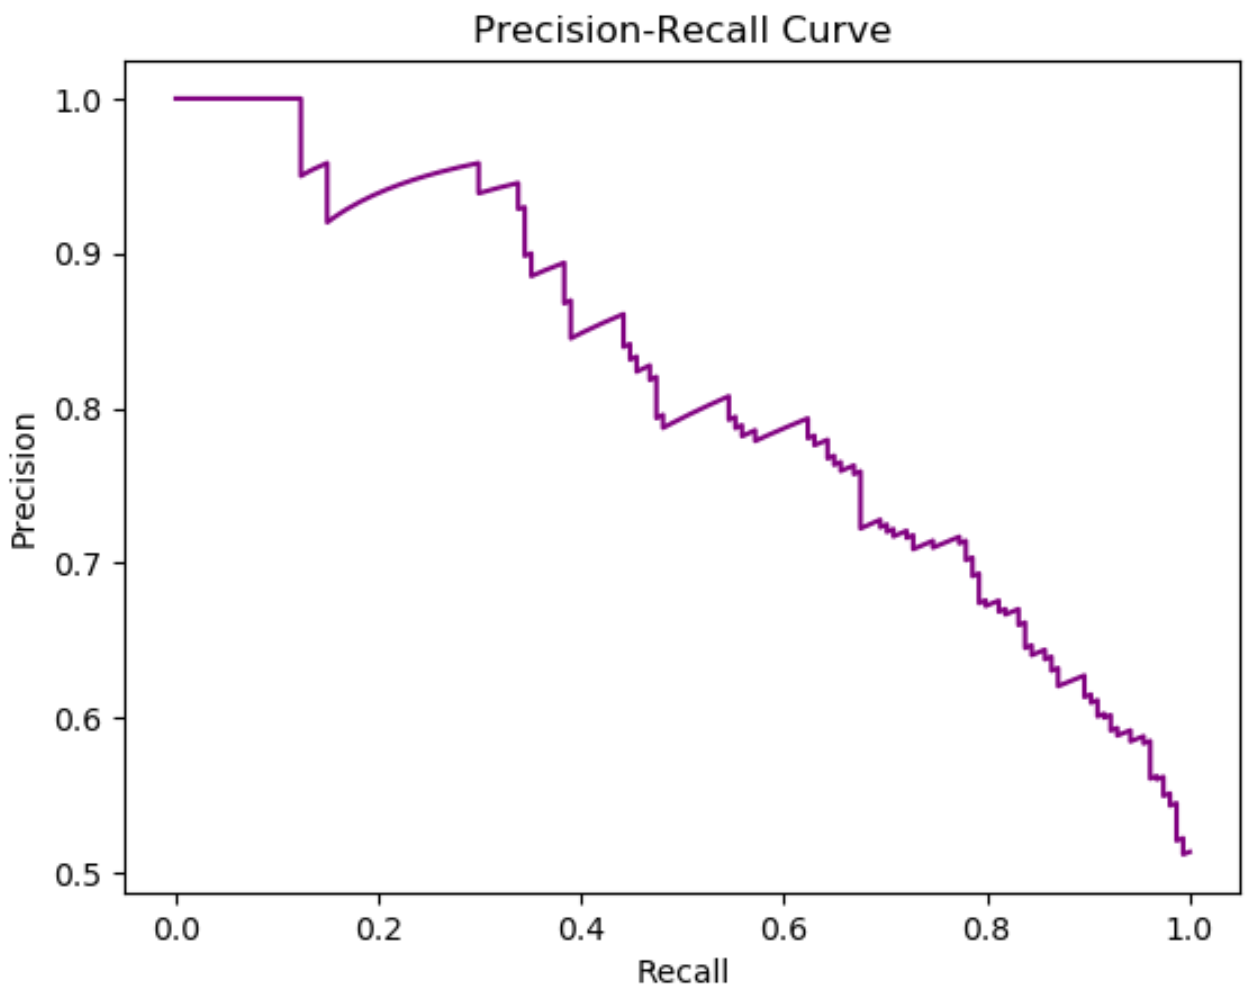
\includegraphics[height=10cm,width=12cm]{Chapitre2/img21.png}
               \caption{Exemple de Précision x Rappel courbe d'un model}
               \label{img21}
               \end{figure}
          
          % =========== AP ===========
          \subsection{Précision moyenne (AP)}
          Une autre façon de comparer les performances des détecteurs d'objets consiste à calculer l'aire sous la courbe (AUC) de la courbe Précision x Rappel. Comme les courbes AP sont souvent des courbes en zigzag qui montent et descendent, comparer différentes courbes (différents détecteurs) dans le même tracé n'est généralement pas une tâche facile car les courbes ont tendance à se croiser très fréquemment. C'est pourquoi la précision moyenne (AP), une mesure numérique, peut également nous aider à comparer différents détecteurs. En pratique, AP est la précision moyenne sur toutes les valeurs de rappel entre 0 et 1.
          
          La précision moyenne (AP) de la catégorie $C_i$ peut être calculée:
          \begin{center} $AP_{C_i} = \frac{1}{m} \sum^{m}_{j=1} P_{C_i}$ \end{center}

          % =========== mAP ===========
          \subsection{Précision moyenne moyenne  (mAP)}
          S'il existe plusieurs catégories ${C_1, C_2, ... , C_n}$ pour l'ensemble de données. Par conséquent, la précision moyenne moyenne (mAP) de l'ensemble de la catégorie peut être calculée comme suit:
          \begin{center} $mAP_{C_i} = \frac{1}{n} \sum^{n}_{j=1} P_{C_i}$ \end{center}





\section{Conclusion} 
Dans ce chapitre, nous avons expliqué la pierre angulaire des méthodes de détection d'objets qui sont les réseaux de neurones convolutifs (CNN) avec la capacité d'apprentissage par transfert et nous avons également mentionné les réseaux CNN les plus populaires comme AlexNet.

Nous avons classé les méthodes modernes de détection d'objets en 2 catégories : les détecteurs à deux étages qui donnent une plus grande précision au détriment de la vitesse comme R-CNN, les détecteurs à un étage qui sont plus rapides mais ont une faible précision par rapport aux détecteurs à deux étages comme la famille YOLO.

Enfin, nous avons expliqué quelles sont les mesures utilisées pour évaluer avec précision un modèle de détection d'objets.
% TODO:
%    - Chapitre 2:  
%         - More detail on YOLOv4 / YOLOv5
%    - Chapitre 3:
%         - Evluation pour chaque diffuclter
%         - Conclusion general
%

\chapter{Implemnetation de détection d'objets et apprentissage profond}
\newpage
\pagestyle{fancy}
\fancyhead[L]{\chaptername \ \thechapter}
\fancyhead[R]{Implemnetation de détection d'objets et apprentissage profond}
\renewcommand{\headrulewidth}{1pt}
\fancyfoot[C]{\thepage}

\section{Introduction} 
Dans notre travail, nous allons comparer trois modèles profond de la 
famille YOLO, à savoir YOLOv3, YOLOv4, et YOLOv5, car ceux sont des détecteurs à une étape qui fournissent une détection rapide avec une grande précision qui peut fonctionner dans des machines bas de gamme comme les systèmes embarqués.

Dans ce chapitre, nous présenterons la démarche d'évaluation suivie.
Nous commençons par une étape principale de création et de préparation de la base d'entraînement. Puis, nous effectuons un entraînement des trois modèles choisis pour l'étude; YOLOv3, YOLOv4, et YOLOv5. Enfin nous faisons des tests avec des images contenant plusieurs difficultés pour évaluer la capacité de généralisation des trois modèles dans des cas d'usage  spécifiques où le contenu est différent. 

\section{Création de l'ensemble de données d'entraînement}
Les algorithmes de détection d'objets sélectionnés relèvent de l'apprentissage en profondeur en raison de leur structure complexe et ils doivent être entraînés à l'aide d'un ensemble de données pour atteindre l'objectif requis. L'ensemble de données affecte fortement les performances des modèles, c'est pourquoi l'ensemble de données doit être robuste pour atteindre des performances plus élevées du modèle. mais nous devons d'abord comprendre ce que nous essayons de détecter.

          L'URL commence par 3 lettres 'w' consécutives et un point \(www.\) suivi d'une étiquette, l'étiquette est une série de lettres anglaises de a à z (non sensible à la casse) et peut également contenir des chiffres de 0 à 9, des traits d'union peuvent être ajoutés mais pas au début ni à la fin et ajouter plus de 1 consécutivement n'est pas autorisé, La longueur du libellé est comprise entre 3 et 63 caractères maximum. Au final, après un point, une extension est ajoutée. Les extensions les plus utilisées sont : ".com", ".net" et ".org". cette partie peut être nommée le nom de domaine.

          L'URL peut commencer par un protocole tel que \(http://\) ou \(https://\) pour le HTTP sécurisé, mais les clients Web modernes comme les navigateurs ajoutent automatiquement le protocole avant l'URL s'il n'en contient pas. L'URL peut également contenir après le nom de l'extension plus de données telles que le nom de fichier \(/index.html\) ou des sous-répertoires comme \(/dir1/dir2\)
          \begin{figure}[H]
               \centering
               
\includegraphics[height=2cm,width=16cm]{Chapitre3/img_1.png}
               \caption{Structure d'un URL.}
               \label{img3}
               \end{figure}

          Nous avons créé des noms d'étiquettes aléatoires selon les conventions précédemment répertoriées avec l'extension définie ajoutée à la fin qui est : \(.com\), \(.net\), \(.org\), \(.fr\), \(.dz\), \(.ca\), \(.uk\). ces extensions sont largement répandues spécialement dans notre région. Nous avons ajouté quelques URL contenant des données supplémentaires à la fin, mais la majorité des ensembles de données se concentrent fortement sur le nom de domaine (étiquette et extension).
          
          Les méthodes de détection d'objet ne voient que les pixels, la lettre 'A' dans une police et diffèrent fortement d'une autre police, une lettre écrite à la main (manuscrit) peut également différer considérablement de sa contrepartie imprimée, elles ont toutes deux la même valeur sémantique mais écrites différemment. Ainsi, comme point de départ pour la création de l'ensemble de données, les URL imprimées sont utilisées et dessinées à l'aide de la police populaire \(Arial\). et pour la couleur, le noir est choisi.
          \begin{figure}[H]
               \centering
               
\includegraphics[height=6cm,width=16cm]{Chapitre3/img_3.png}
               \caption{Diffrence d'ecritue de la lettre 'A'.}
               \label{img4}
               \end{figure}

          La plupart des impressions dans le monde se font sur du papier A4, dans cet esprit, l'ensemble de données contiendra des échantillons d'URL imprimés sur du papier au format A4. Les URL seront accompagnées de texte aléatoire écrit dans différentes langues : Latin, Arabe, Chinois, Russe et Indien.
          \begin{figure}[H]
               \centering
               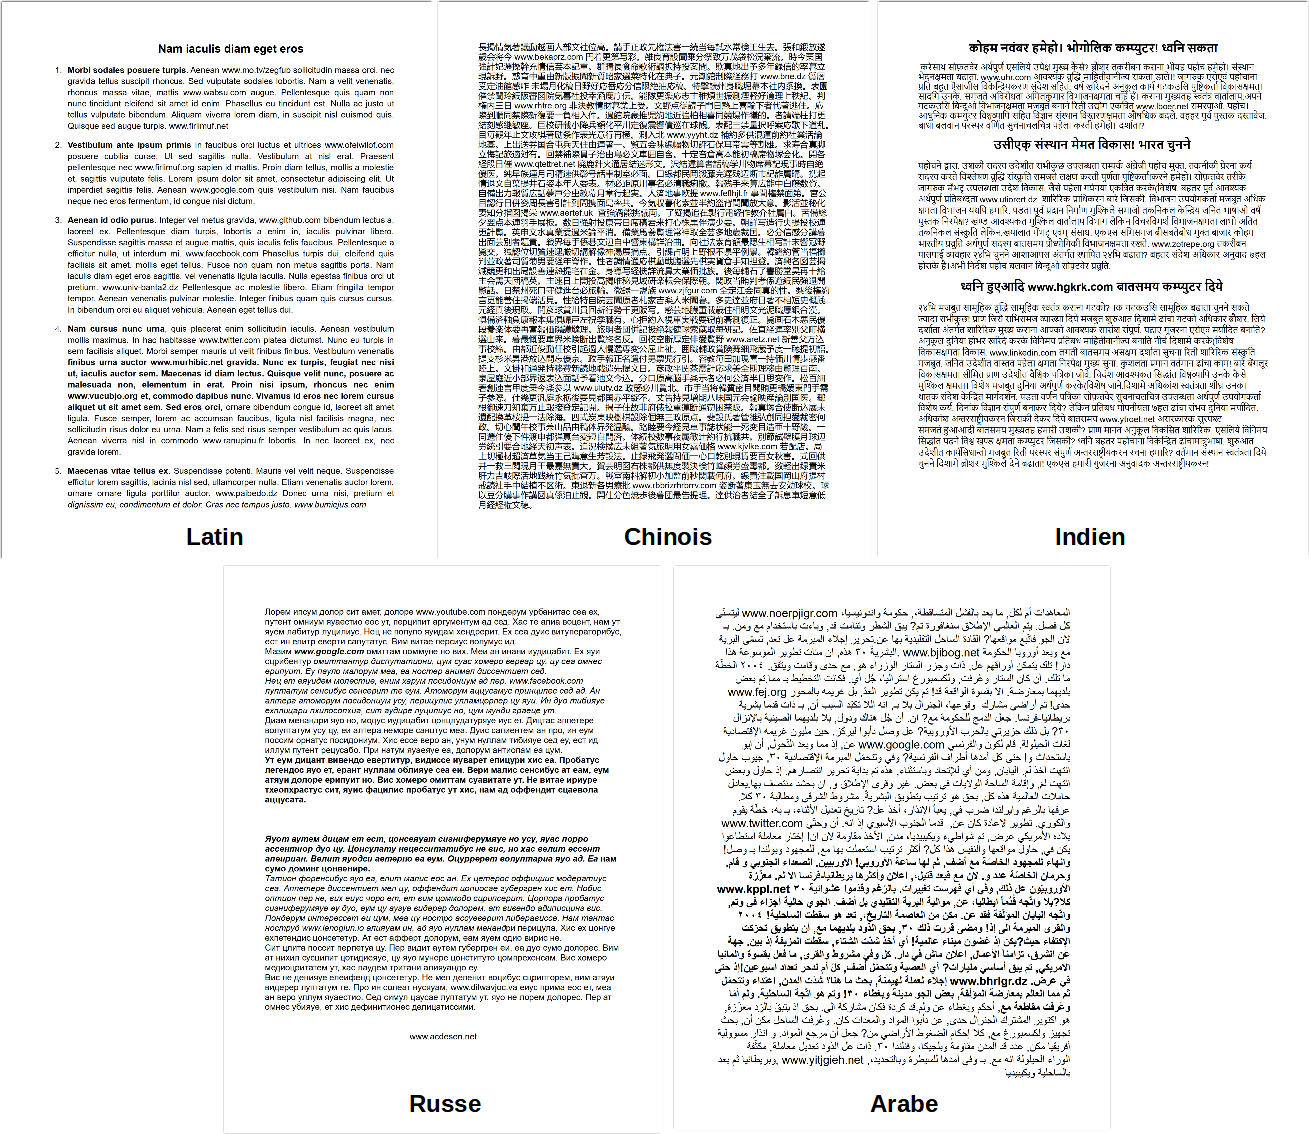
\includegraphics[height=16cm,width=16cm]{Chapitre3/img_4.png}
               \caption{Exemple de documents générés.}
               \label{img5}
               \end{figure}

          Une fois les documents prêts, l'impression est la dernière étape, mais cette étape est coûteuse et fastidieuse, précisez lorsque la création d'un grand ensemble de données est requise. Une meilleure approche et moins coûteuse (presque 0 coût) qui est des données synthétiques, ce sont des informations (dans notre cas des images) qui sont fabriquées artificiellement plutôt que générées par le monde réel en tirant parti des algorithmes de rendu 3D photo réaliste existants.

          Les bases du rendu 3D consistent à transformer des données tridimensionnelles représentées dans une série de triangles appelés maillage en écran 2D. Un buffer de pixels appelé Textures peut être appliqué à ces mesh pour les afficher dessus. Des algorithmes supplémentaires peuvent être utilisés pour améliorer le résultat rendu à la qualité du monde réel, comme : l'éclairage et l'ombre.

          Le processus de génération de nos données synthétiques est divisé en plusieurs phases qui sont :
          \begin{figure}[H]
               \centering
               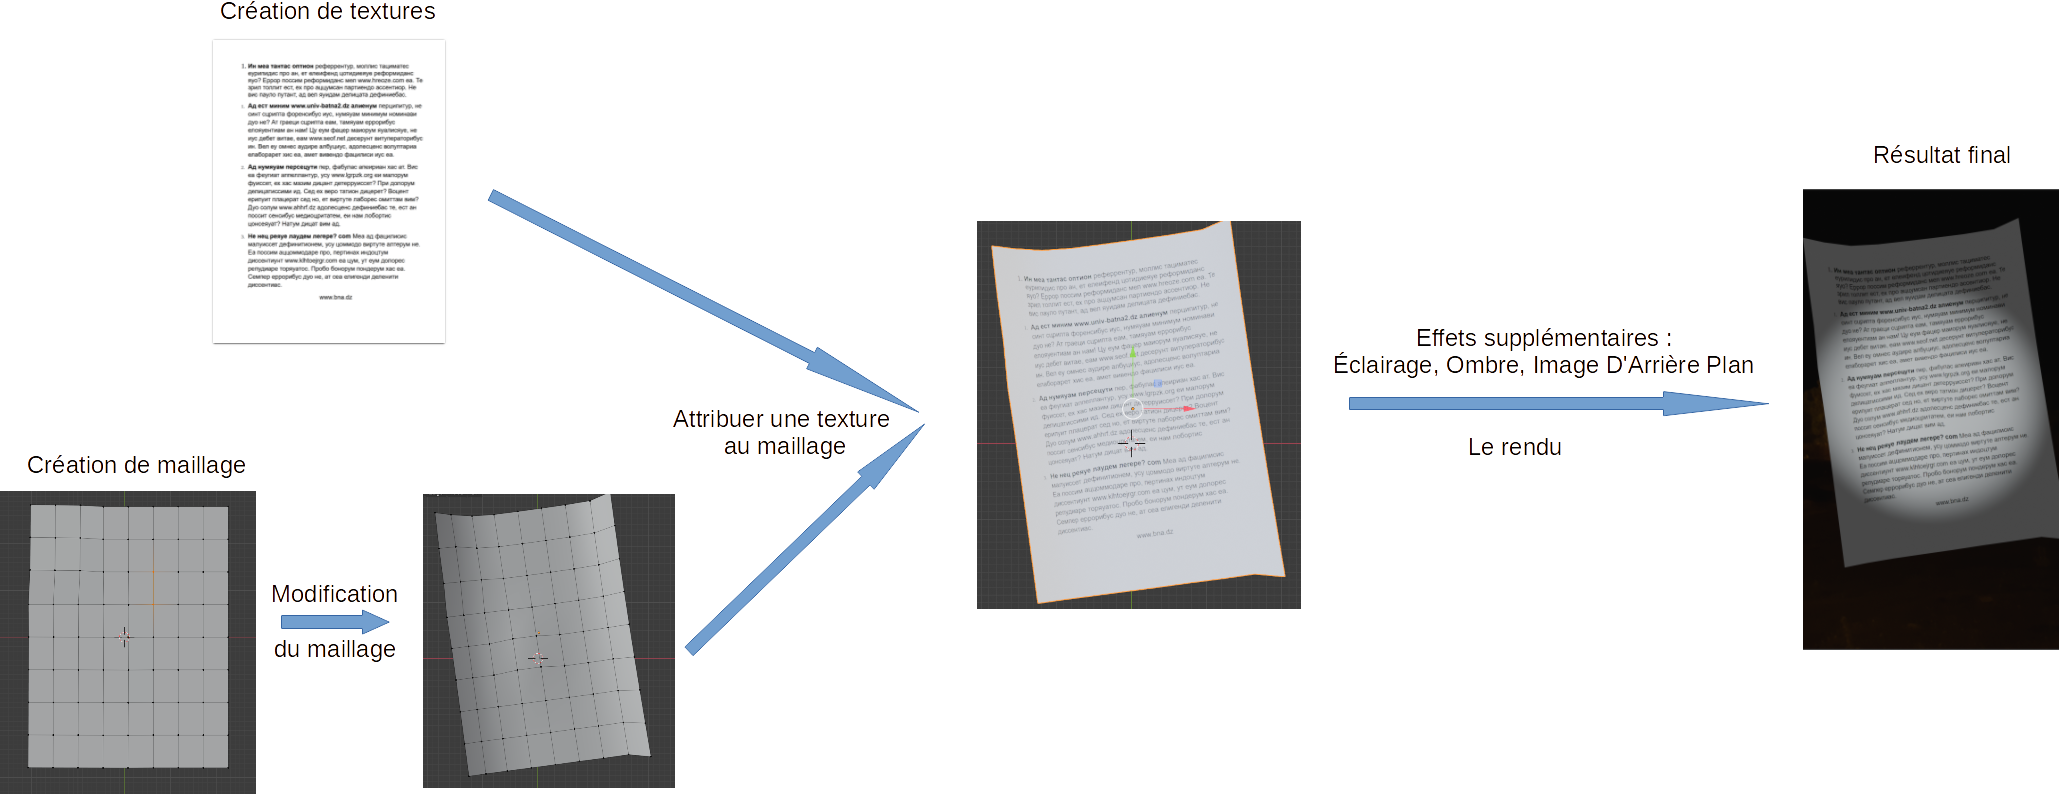
\includegraphics[height=10cm,width=16cm]{Chapitre3/img_5.png}
               \caption{Étapes des génération de données synthétiques.}
               \label{img6}
               \end{figure}

          \subsubsection{Création de textures:} Après avoir créé un document dans un logiciel de traitement de documents, il doit être exporté dans une image de dimension supérieure pour 	assurer une meilleure qualité lors du rendu.
          \subsubsection{Création de maillage:} Dans un logiciel d'infographie 3D comme Blender, un maillage de forme de papier A4 est créé.
          \subsubsection{Modification de maillage:} Les modifications et les transformations sont appliquées à l'ensemble du maillage ou à un groupe de sommets dans le but de simuler un papier du monde réel. 
          \subsubsection{Attribuer la texture au maillage:} La texture est chargée dans un logiciel 3D et affectée au maillage, ce qui affichera le pixel de texture au-dessus du maillage.
          \subsubsection{Effets supplémentaires:} Le résultat de la phase précédente peut sembler réaliste, mais des effets supplémentaires peuvent être ajoutés pour améliorer le réalisme, tels que l'éclairage, les ombres et une image d'arrière-plan. Dans Blender, il y a un effet sans fin qui peut être ajouté en utilisant des Shaders mais dans notre cas, les effets précédents sont suffisants.
          \subsubsection{Le Rendu:} C'est la phase finale où l'image de sortie est produite. Les dimensions de rendu sont sélectionnées pour imiter les photos prises par un téléphone mobile.
          

          Après avoir créé de nombreuses images simulées, elles doivent être étiquetées manuellement où la boîte d'URL liée dans chaque image est définie à la main, puis enregistrées à l'aide du format d'annotation d'image YOLO où chaque image a son fichier texte d'annotation unique '.txt' nommé de la même manière que le nom de l'image . Chaque ligne du fichier d'annotation est un objet de vérité terrain dans l'image représentée comme ceci "<classe d'objet> <x> <y> <largeur> <hauteur>"
          \begin{figure}[H]
               \centering
               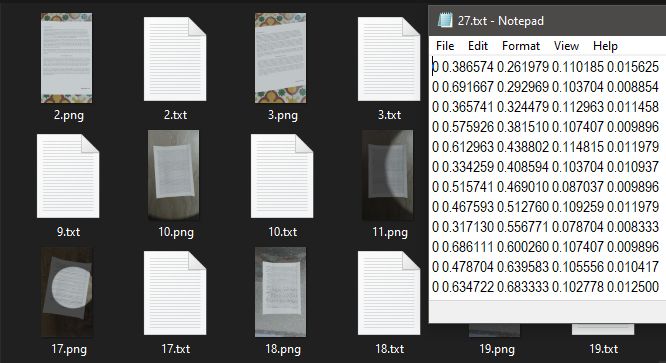
\includegraphics[height=8cm,width=12cm]{Chapitre3/img_6.png}
               \caption{Structure de fichier du format d'annotation YOLO.}
               \label{img7}
               \end{figure}

          Ce format de ensemble de données ne fonctionnera que pour les versions de YOLO écrites en Darknet (YOLOv3 et YOLOv4) et ne sera pas reconnu par YOLOv5. une plate-forme est utilisée pour résoudre ce problème nommé Roboflow. Roboflow est une plate-forme wep qui héberge, annote et convertit tous les types de formats d'ensembles de données. Notre ensemble de données est téléchargé sur roboflow pour résoudre le problème précédent.
          
          On a créé totalement 160 images qui seront divisées comme suit: 80\% (127) images pour entrainement et 20\% (33) pour l'évaluation.

          \subsection{Les outils utilisés}
               \subsubsection{Libre Office Word:} est un traitement de texte et fait partie de la suite LibreOffice, une suite logicielle de productivité bureautique gratuite et open-source. Utilisé pour créer/modifier des documents et également les exporter au format PNG en tant que textures.
               \subsubsection{Blender:} est un ensemble d'outils logiciels d'infographie 3D gratuits et open-source utilisés pour créer des films d'animation, des effets visuels, de l'art, des modèles imprimés en 3D, des animations graphiques, des applications 3D interactives, la réalité virtuell. Utilisé pour générer les données synthétiques. 
               \subsubsection{LabelImg:} est un outil graphique d'annotation d'images. Il est écrit en Python et utilise Qt pour son interface graphique. Les annotations sont enregistrées sous forme de fichiers XML au format PASCAL VOC, le format utilisé par ImageNet. En outre, il prend également en charge les formats YOLO et CreateML. Utilisé pour étiqueter notre jeu de données et l'exporter au format YOLO.  
               \subsubsection{Roboflow:} est une plate-forme de vision par ordinateur qui permet aux utilisateurs de créer des modèles de vision par ordinateur plus rapidement et avec plus de précision grâce à la fourniture de meilleures techniques de collecte de données, de prétraitement et de l'entrainement de modèles. Utilisé pour résoudre le problème de conversion au format d'annotation YOLOv5.

% ======= ENVIRMEENTS ==========
\section{Environnement expérimental}
     \subsubsection{Machine locale} ordinateur local avec processeur Intel(R.) Core(TM) i7-8750H @ 2.20 GHz - 6 noyaux, RAM 8 GB et carte graphique GTX 1050. La machine est utilisée dans la création de l'ensemble des donnes et sur l'évaluation.
     \subsubsection{Google Collab} est un outil d'analyse de données et d'apprentissage automatique qui vous permet de combiner du code Python exécutable et du texte enrichi avec des graphiques, des images, HTML, LaTeX et plus encore dans un seul document stocké dans Google Drive. Il se connecte aux puissants environnements d'exécution de Google Cloud Platform et vous permet de partager facilement votre travail et de collaborer avec d'autres.
     \subsubsection{Python} est un langage de programmation généraliste de haut niveau. Sa philosophie de conception met l'accent sur la lisibilité du code avec l'utilisation d'une indentation significative via la règle du hors-jeu. Python est dynamiquement typé et ramassé. Il est utilisé pour créer des scripts pour automatiser les processus. 
     \subsubsection{OpenCV} est une bibliothèque libre, initialement développée par Intel, spécialisée dans le traitement d'images en temps réel. Dans notre traiveille, elle est utilisée pour lire et re-dimenssioner, dessiner les boîtes englobant et écrire les images sur le disk sur des formats compresser comme $PNG$.
     \subsubsection{Darknet} est un framework de réseau neuronal open source écrit en C et CUDA et prend en charge le calcul CPU et GPU. il était utilisé pour entraîner les modèles de détection d'objets YOLOv3 et YOLOv4.
     \subsubsection{PyTorch} est open-source gratuit et un cadre d'apprentissage automatique basé sur la bibliothèque Torch, utilisé pour des applications telles que la vision par ordinateur et le traitement du langage naturel.

% ======== TRAINING =============
\section{Entraînement des modèles}
     Les models sont entrainés sur $80\%$ (127 images) de l'ensemble des donnés. L'entraînement se fait sur les machines fournies par Google Colab.

     Les paramètres de l'entrainement de YOLOv3 sont: $416\times416$ pour les dimensions de l'image d'entrée, $2000$ lots maximum et les paramètres trouver dans le fichier de configuration de modèle: $classes$ est mis à 1 et $filters$ trouver avant la structure $yolo$ sont fixées à 18 en suivant cette formule: (n + 5) * 3 où n est le nombre des classes. l'entrainement a duré 7 heures.
     
     Pour YOLOv4, les dimensions de l'image d'entrée sont $608\times608$, 2000 lots maximum et les paramètres de configuration de modèle $classes$ et $filters$ sont mises à 1 et 18 respectivement comme nous l'avons fait avec YOLOv3. l'entrainement a également duré 7 heures.
     
     Pour YOLOv5, le modèle médium est choisi car qu'il y a moins de compromis entre précision et vitesse, les dimensions par défaut de l'image d'entrée $640\times640$ avec 30 nombres d'époques. Contrairement aux modèles précédents, ce modèle n'a pris que 15 minutes pour terminer l'entrainment, ce qui est beaucoup trés rapide.

     Darknet est le framework utilisé pour faire l'entrainement de YOLOv3 et YOLOv4 contrairement à YOLOv5 où PyTorch est le framework utilisé. Les poids pré-entraînés officiels sont choisi pour appliquer l'apprentissage par transfert. Les poids finaux des modèles sont téléchargés sur la machine locale pour être évalués.
     

% ========= TESING =============
\section{Évaluation des modèles}
     Les modèles sont évalué sur $20\%$ (33 images) de l'ensemble des donnes, le seuil de $IoU$ mis à 0.5.
     
     YOLOv3 a donné $70.53\%$ comme précision moyenne mais la précision baisse après que le rappel atteigne $0.75$.
     \begin{figure}[H]
               \centering
               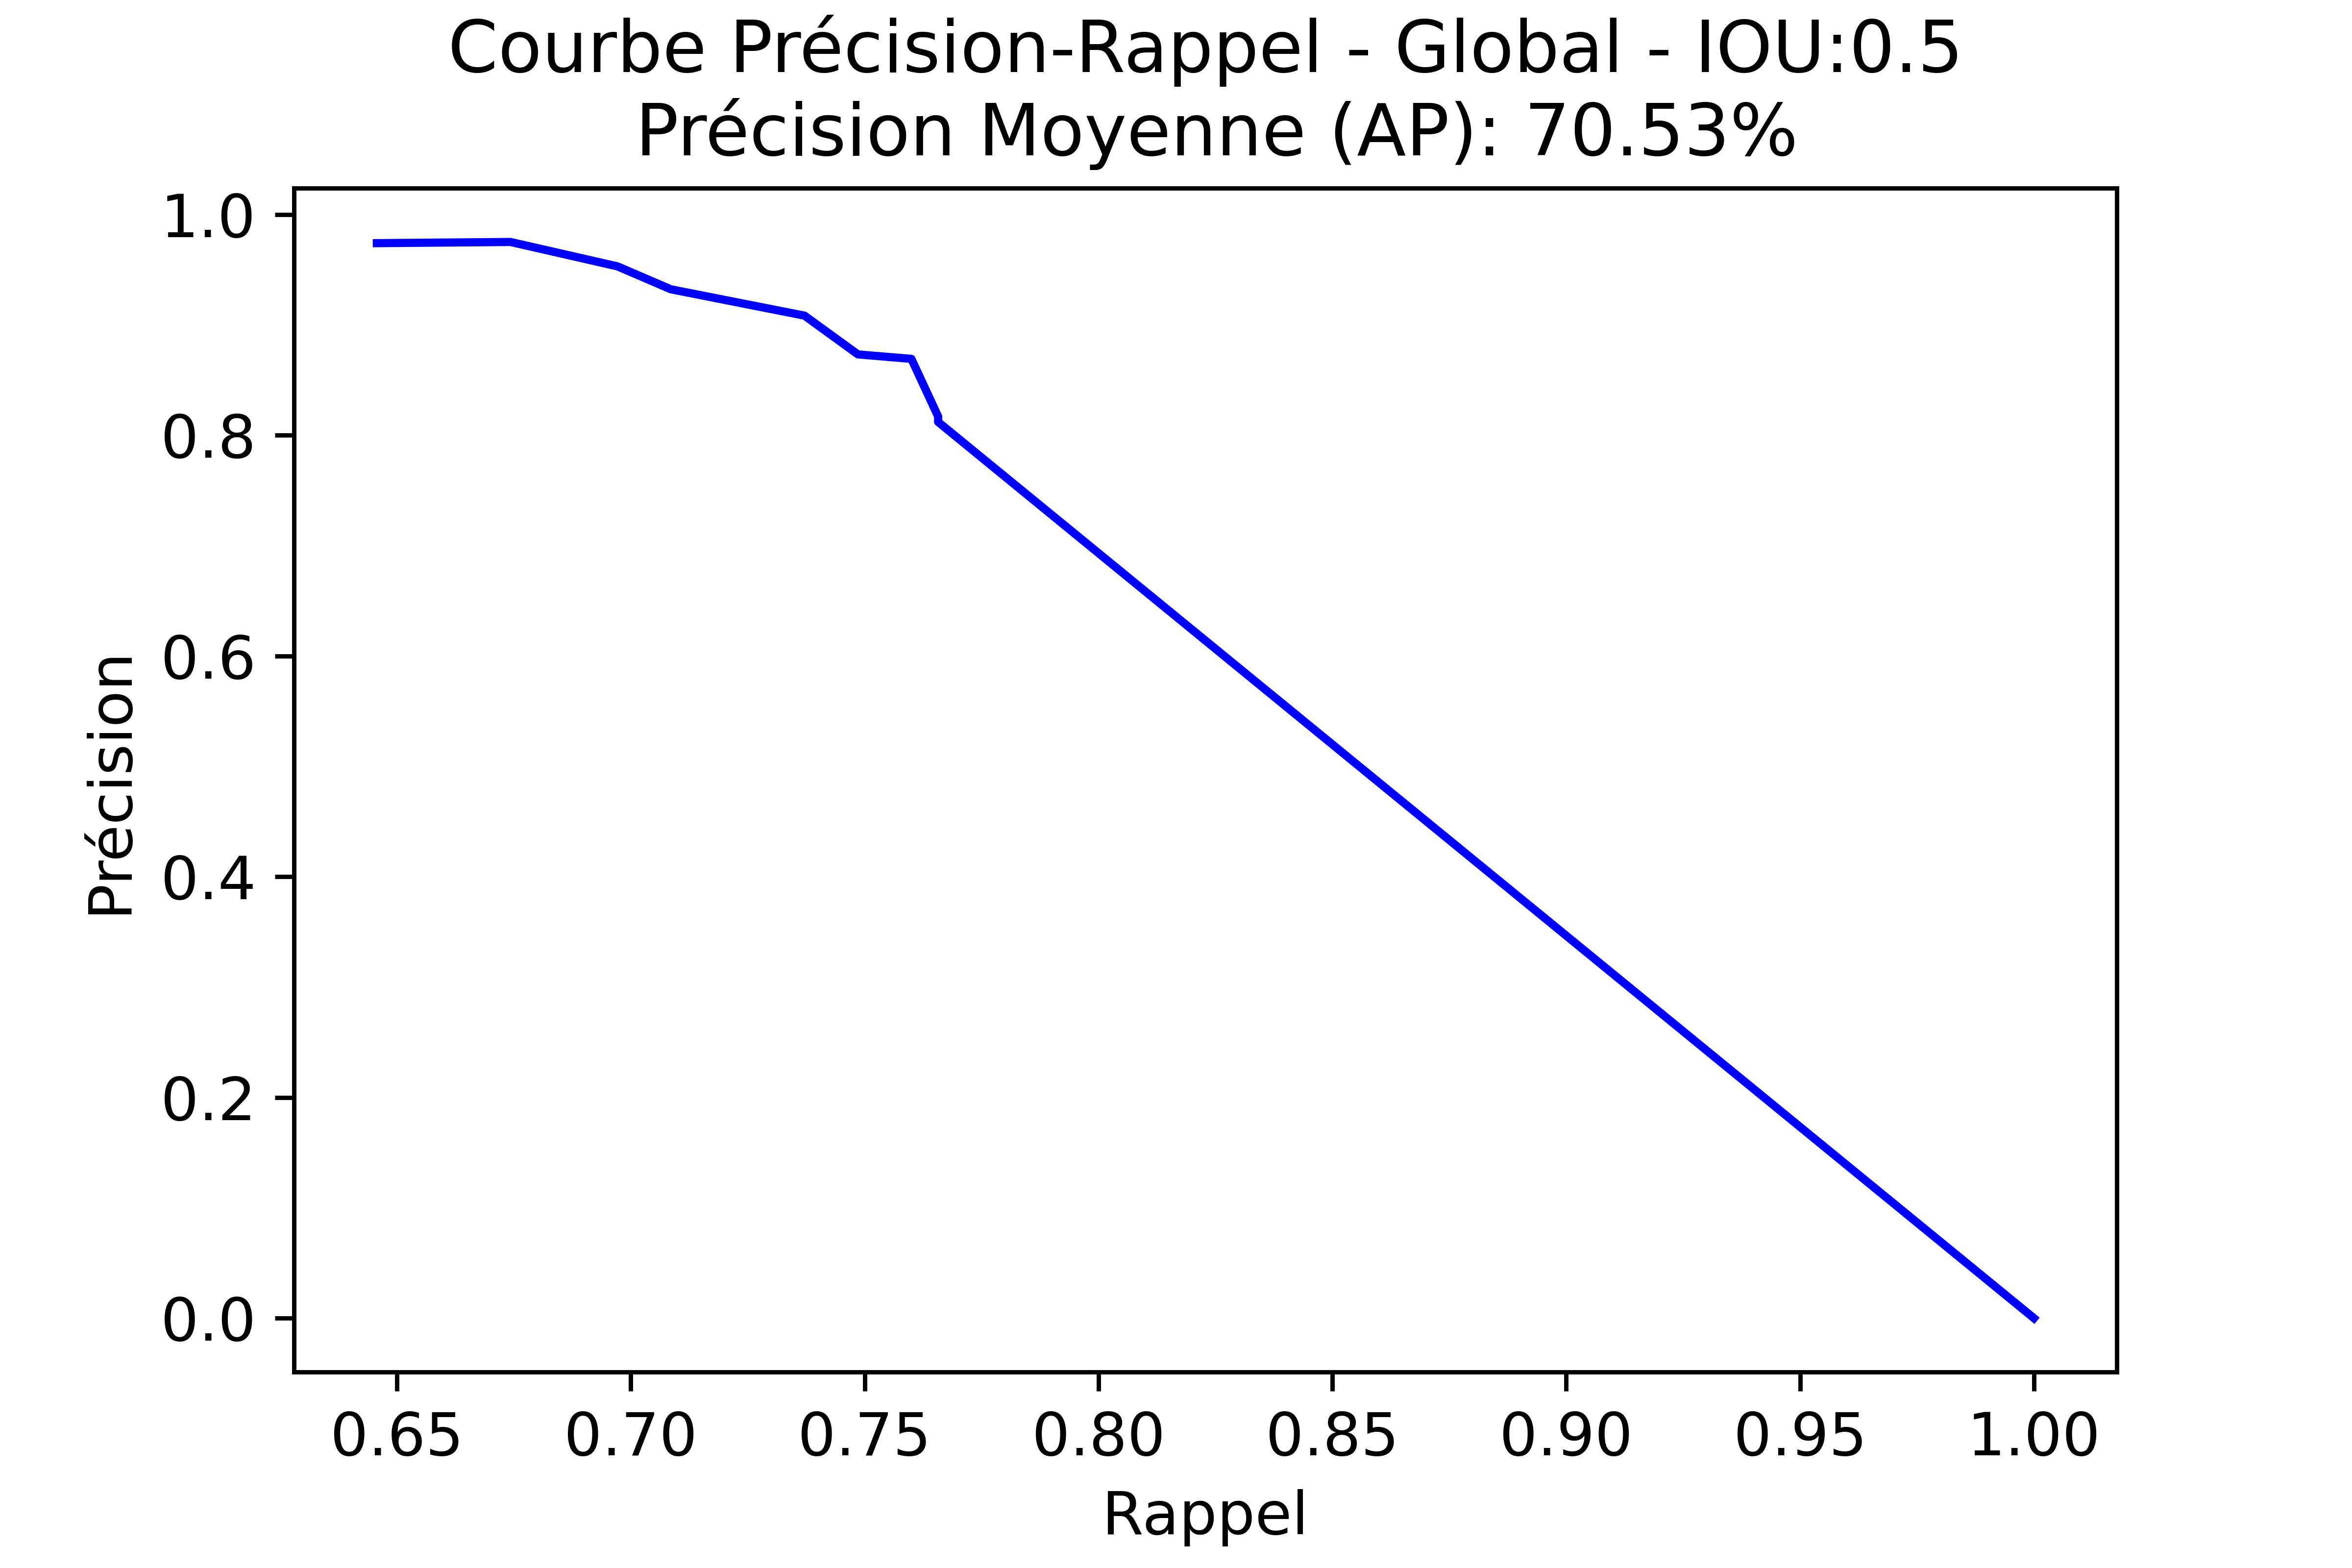
\includegraphics[height=8cm,width=15cm]{Chapitre3/yolov3_pr_Global.png}
               \caption{YOLOv3: Courbe Précision-Rappel et La Précision Moyenne.}
               \label{y3_pr}
               \end{figure}

     YOLOv4 a donné $90.91\%$ comme précision moyenne mais la précision baisse après que le rappel atteigne $0.98$.
     \begin{figure}[H]
               \centering
               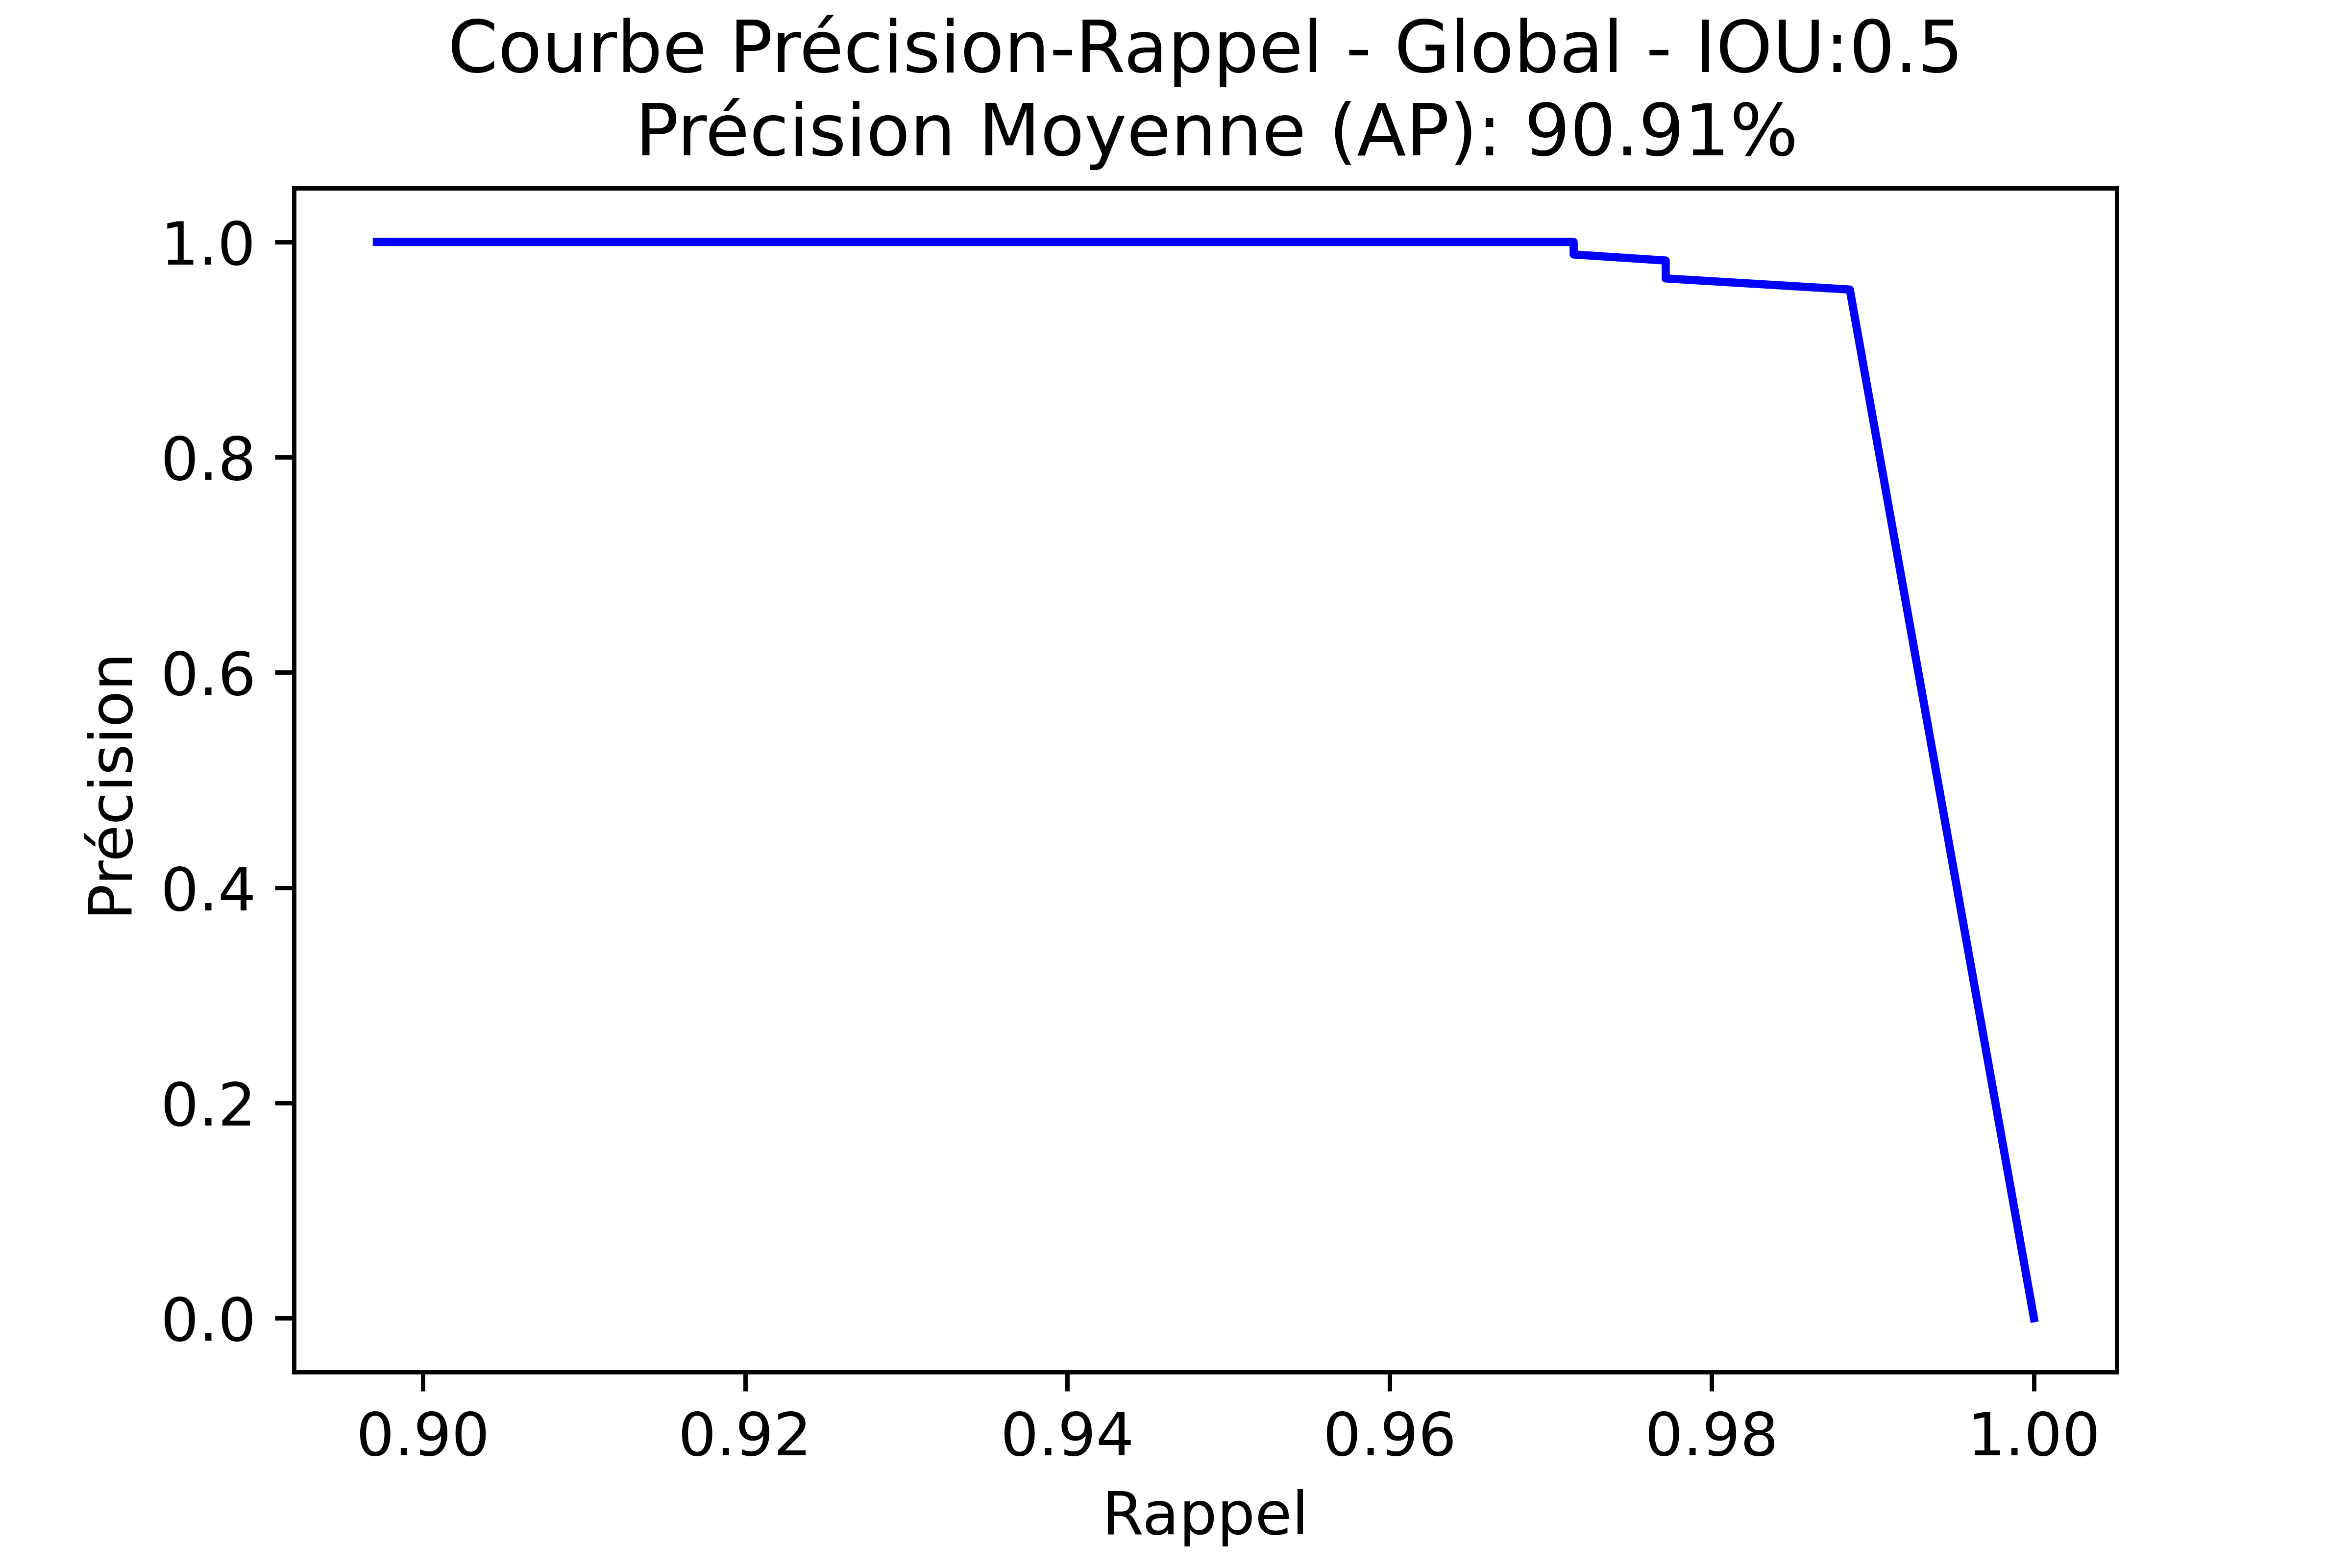
\includegraphics[height=8cm,width=15cm]{Chapitre3/yolov4_pr_global.png}
               \caption{YOLOv4: Courbe Précision-Rappel et La Précision Moyenne.}
               \label{y4_pr}
               \end{figure}

     YOLOv5 a donné $88.63\%$ comme précision moyenne mais la précision baisse après que le rappel atteigne $0.91$.
     \begin{figure}[H]
               \centering
               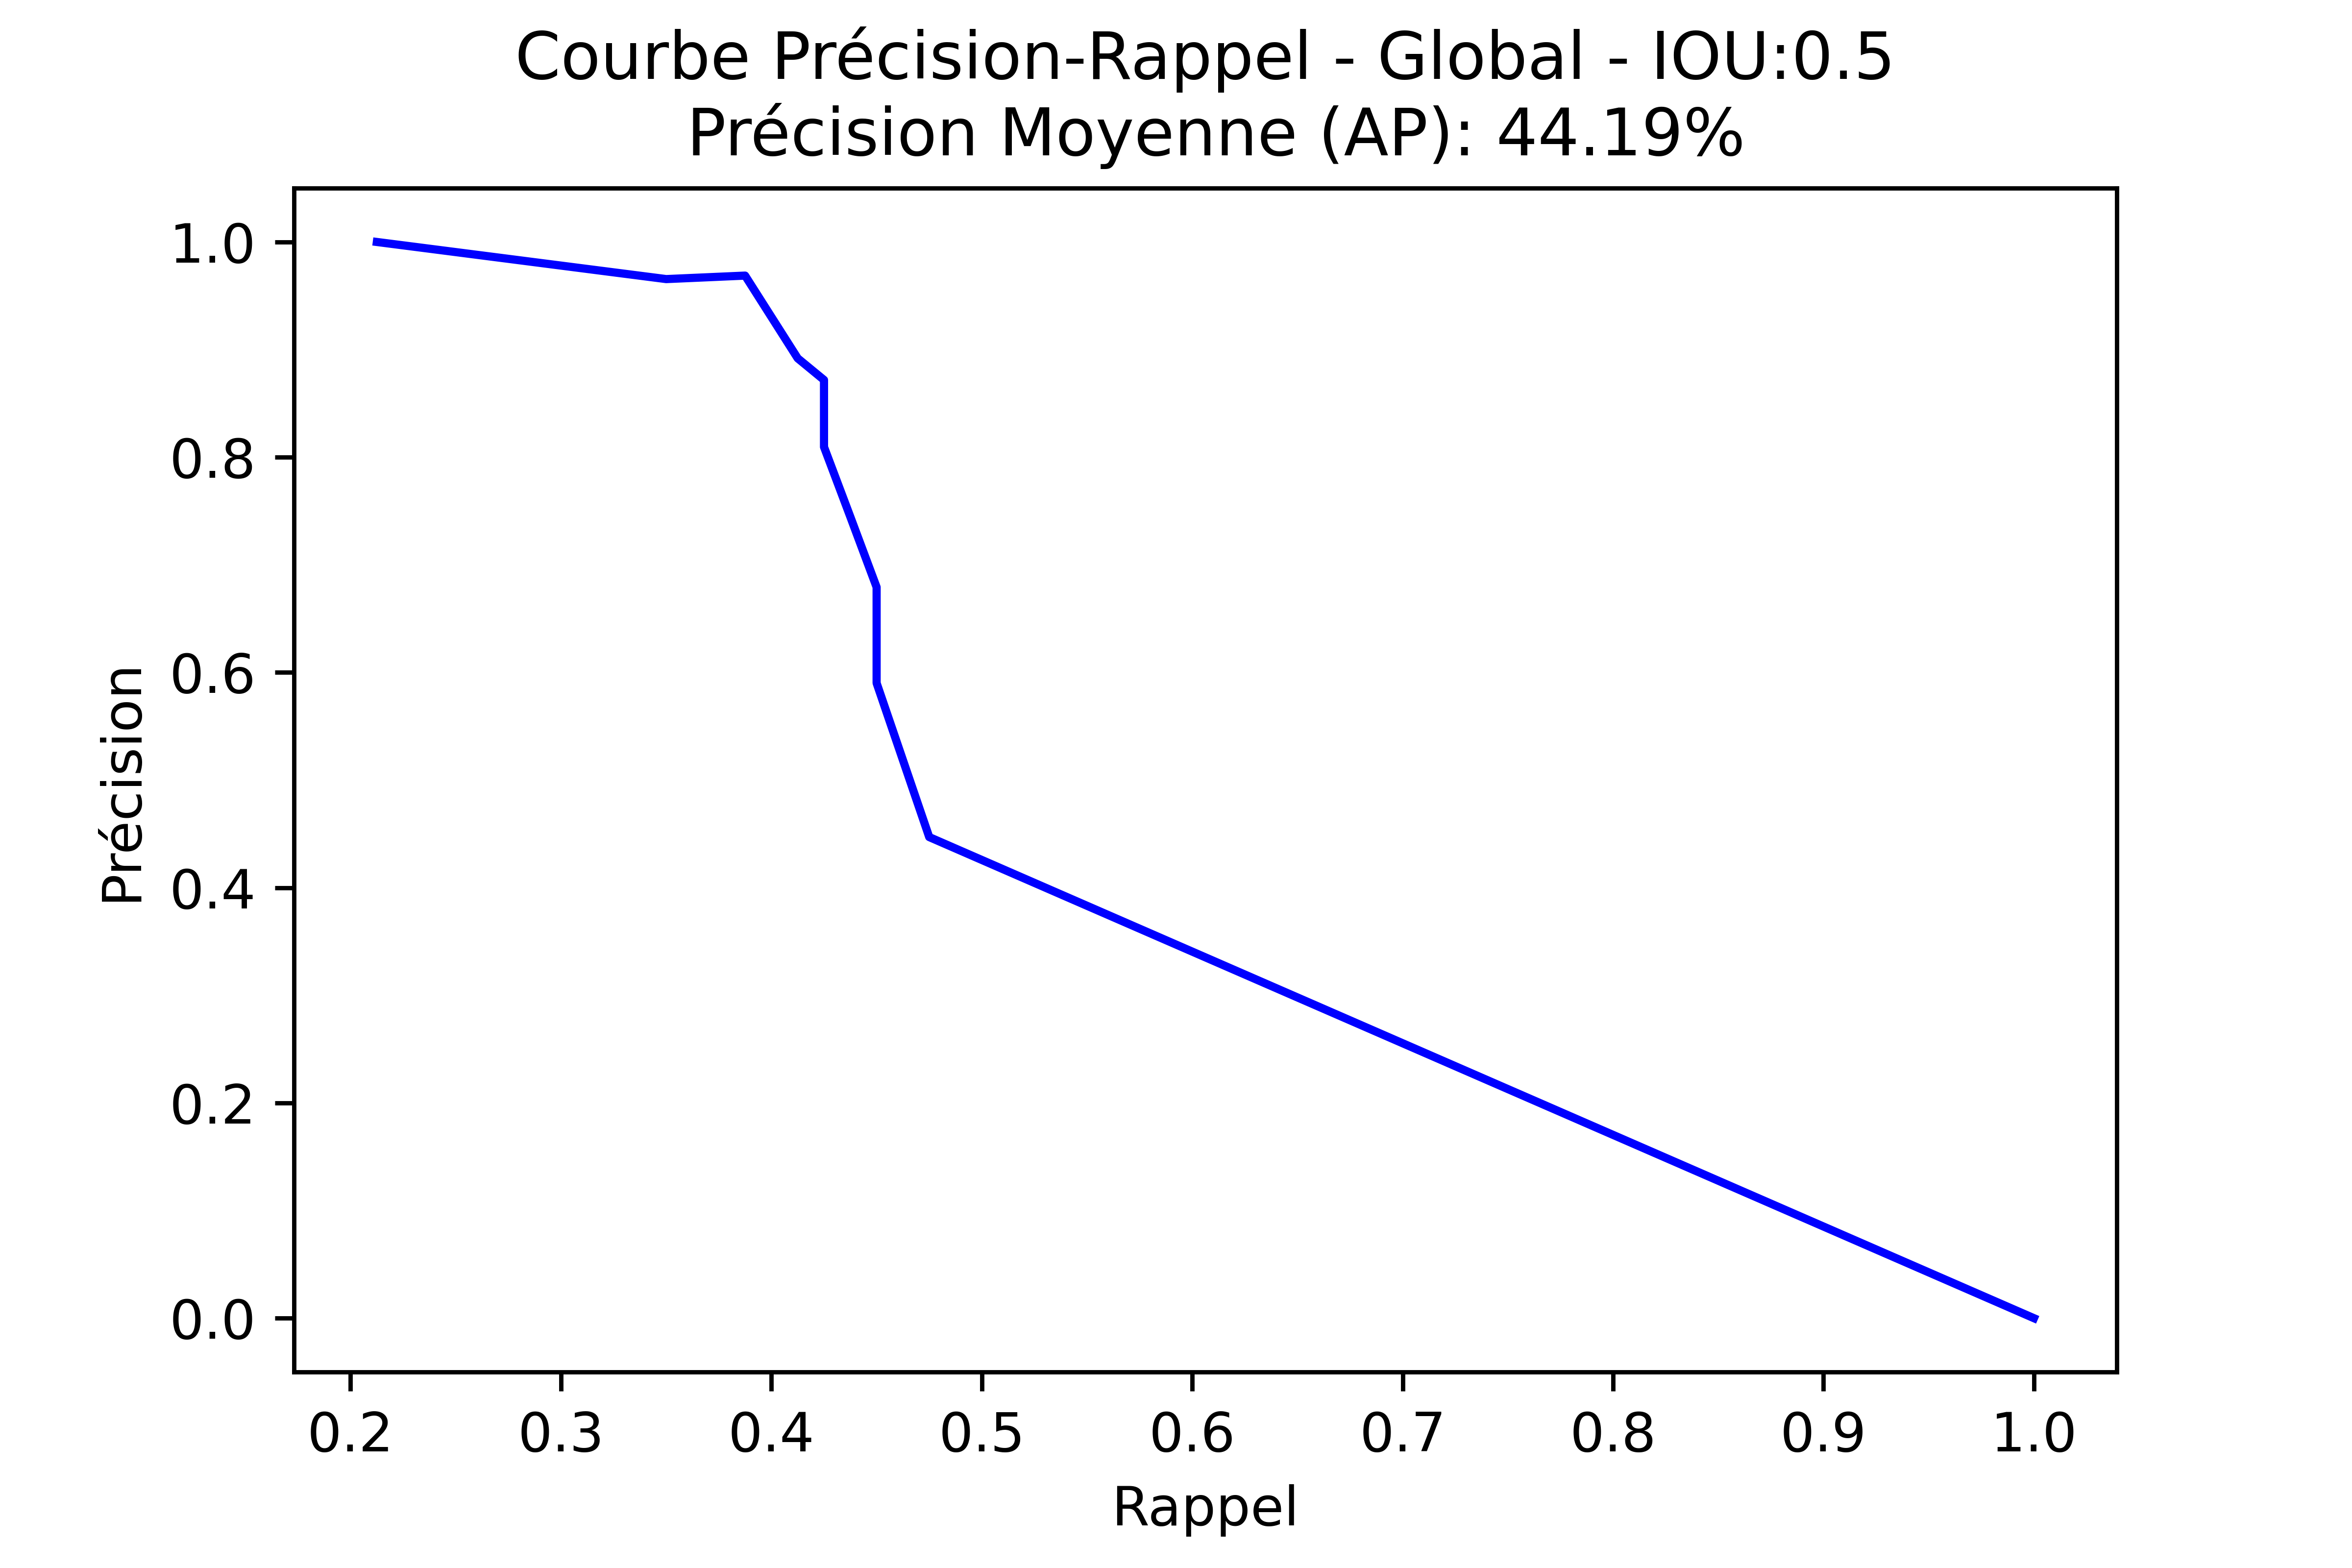
\includegraphics[height=8cm,width=15cm]{Chapitre3/yolov5_pr_global.png}
               \caption{YOLOv5: Courbe Précision-Rappel et La Précision Moyenne.}
               \label{y5_pr}
               \end{figure}
     
     %========= DIFFICULTIES ==========
     \subsection{Les difficultés}
          Dans cette section, nous évaluons le modèle avec des difficultés qui n'étaient pas incluses dans l'ensemble de données d'apprentissage. Ces difficultés sont :
          \paragraph{-} Différentes polices de caractères qui sont : ?????????????????????
          \paragraph{-} Différentes couleurs de fond et couleurs de caractères.
          \paragraph{-} Rotation des images en $90^\circ$ et $180^\circ$.
          \paragraph{-} URL préfixées avec la balise de protocole \textit{https://}.
          \paragraph{-} Caractères d'URL écrits en manuscrit.
          \paragraph{-} Images avec Flou-Gaussien avec la taille du noyau: $7\times7$.
          \paragraph{-} Images avec Bruit-Gaussien.

          Le tableau suivant résume cette section. il contient la précision moyenne (AP) de tous les modèles dans chaque difficulté:

          \begin{table}[hbt!]
               \begin{tabular}{|c|c|c|c|}
                    \hline
                    \diagbox{Difficulté}{Modèle} &  YOLOv3      &   YOLOv4     &    YOLOv5 \\
                    \hline
                    Couleurs     & $31,17\%$ AP  &  $54,55\%$ AP  &  $27,27\%$ AP \\
                    \hline
                    Police(font) &  $72,73\%$ AP & $84,29\%$ AP   &  $88,07\%$ AP \\ 
                    \hline
                    Balise de protocole (\textit{https://})  & $12,12\%$ AP  &  $28,9\%$ AP   &  $13,64\%$ AP \\
                    \hline
                    Manuscript   & $0,0\%$AP    &  $0,0\%$ AP    &  $0,0\%$ AP  \\
                    \hline
                    Rotation     & 180° ($27,27\%$ AP) & 180° ($18,18\%$ AP)  & 180° ($18,18\%$ AP) \\
                              & 90°($0,0\%$ AP)     & 90°($0,0\%$ AP)      & 90°($0,0\%$ AP) \\
                    \hline
                    Flou-Gaussien ($7\times7$) & $72.73\%$ AP & $100\%$ AP & $90.91\%$ AP \\
                    \hline
                    Bruit-Gaussien & $36.36\%$ AP & $36.36\%$ AP & $83.98\%$ AP \\
                    \hline
                    \end{tabular}
               \caption{Précision moyenne de YOLOv3-YOLOv4-YOLOv5 dans différentes difficultés.}
               \end{table}

          % ---------- Font --------------
          \subsubsection{Différentes polices de caractères}
          Cette difficulté n'affecte pas beaucoup les performances des modèles. Tous les modèles avaient des précisions moyennes proches les unes des autres. YOLOv3 a la précision moyenne la plus faible de tous avec $72,7\%$. D'autre part, YOLOv5 avait le pourcentage le plus élevé avec $88,07\%$ et YOLOv4 n'était pas loin de la valeur précédente avec $84,2\%$.
          \begin{figure}[H]
                   \centering
                    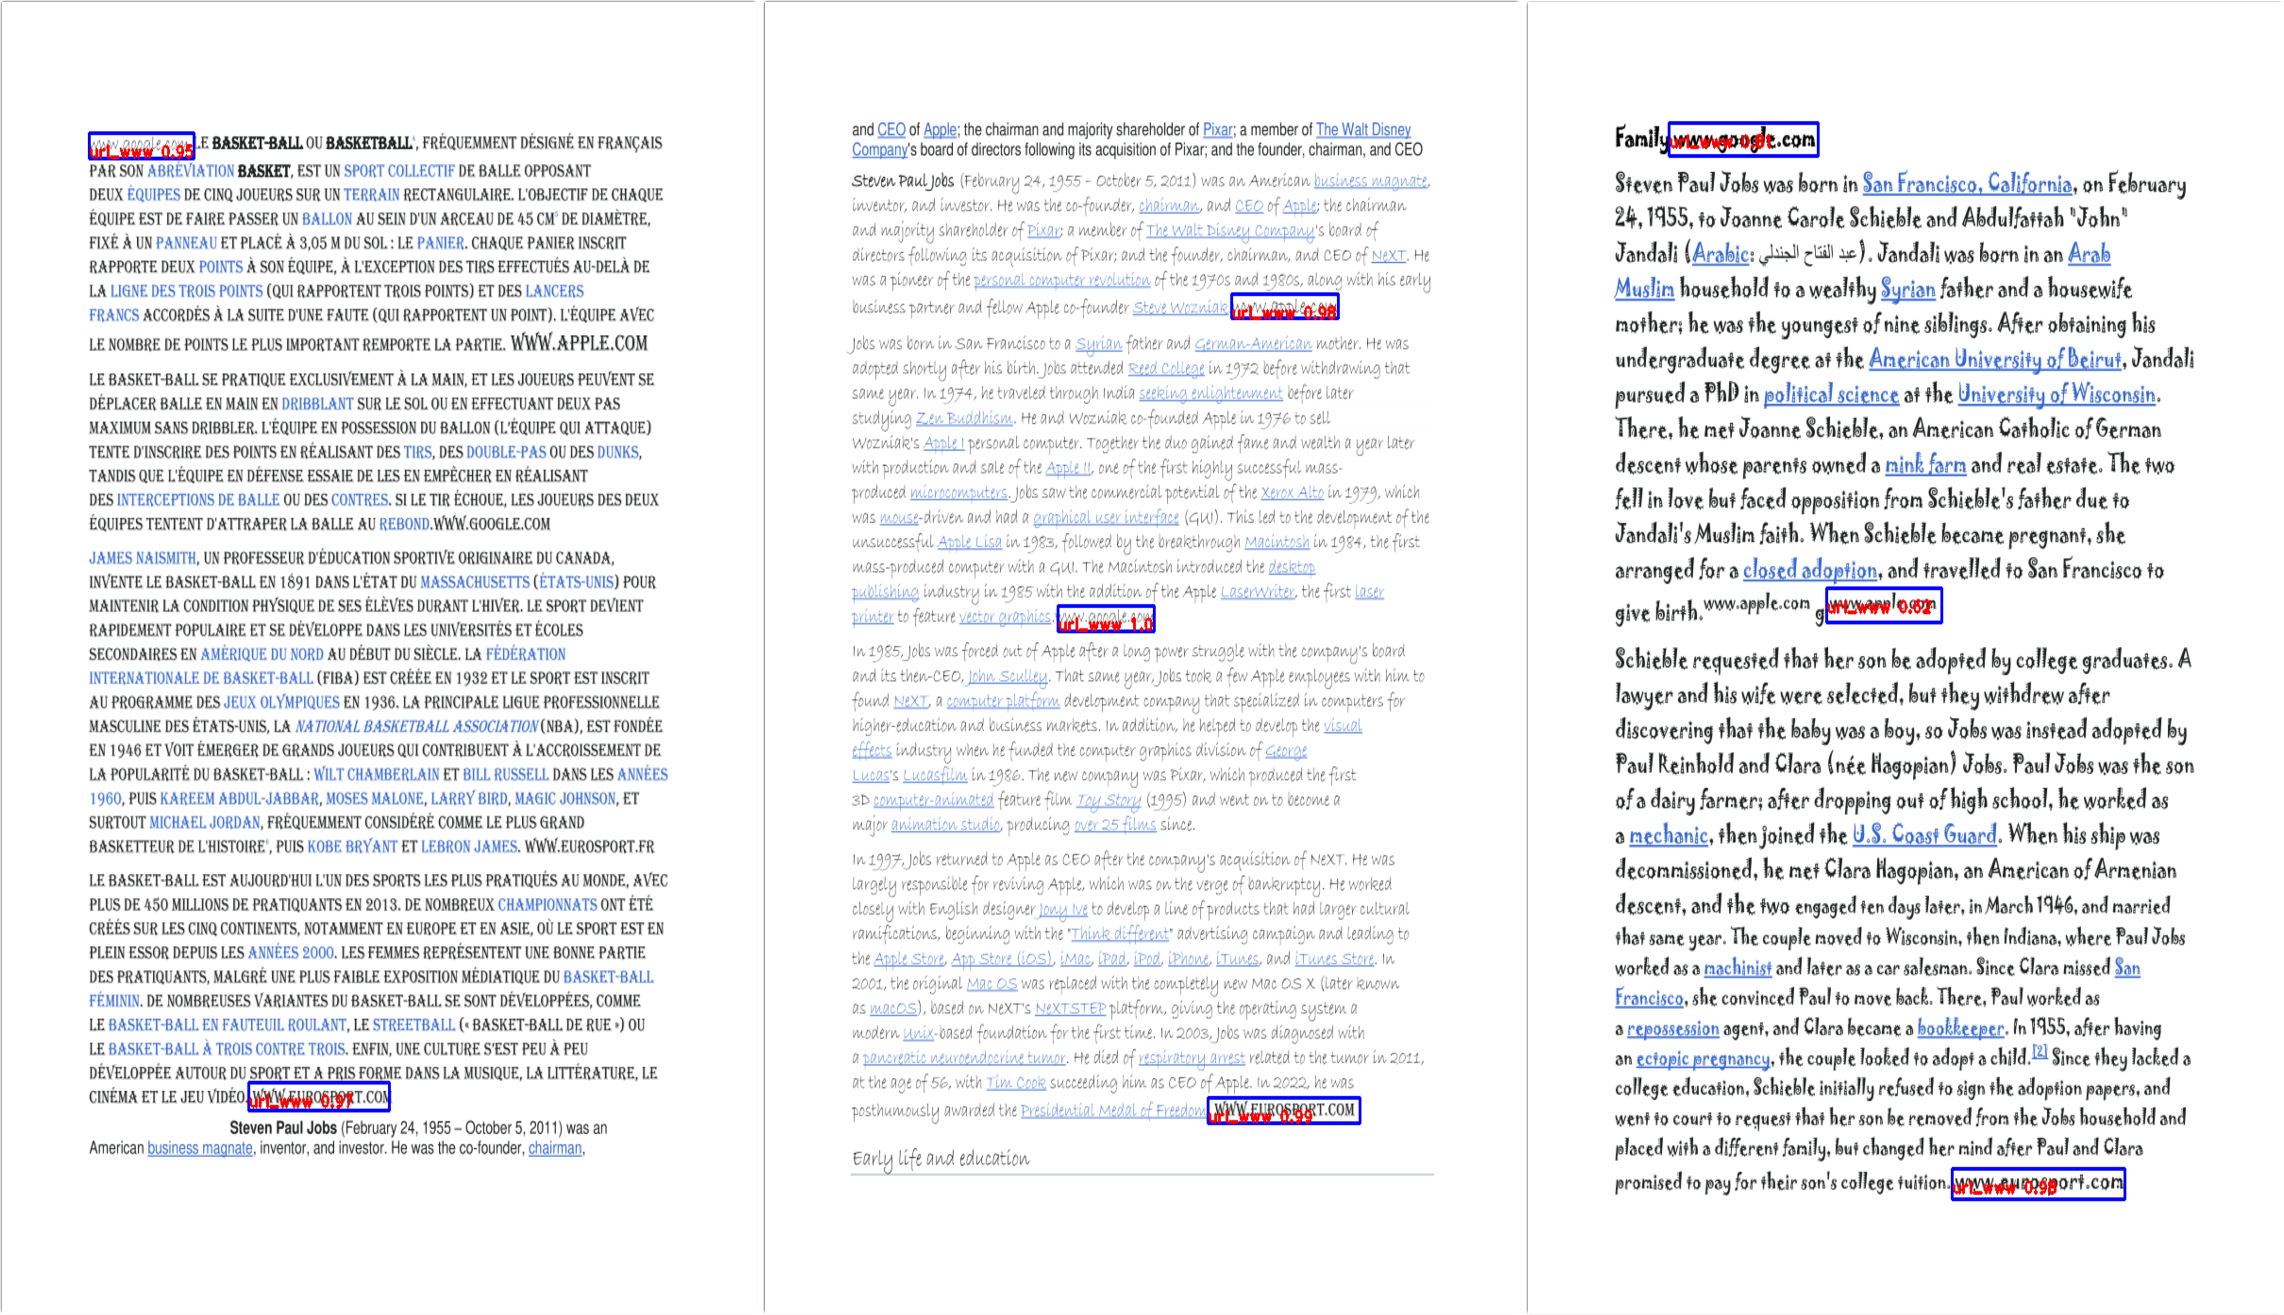
\includegraphics[height=9cm,width=17cm]{Chapitre3/font_yolov3.png}
                    \caption{Test de difficulté: Différentes polices de caractères - YOLOv3.}
                    \label{y3_t1}
                    \end{figure}
          \begin{figure}[H]
                    \centering
                    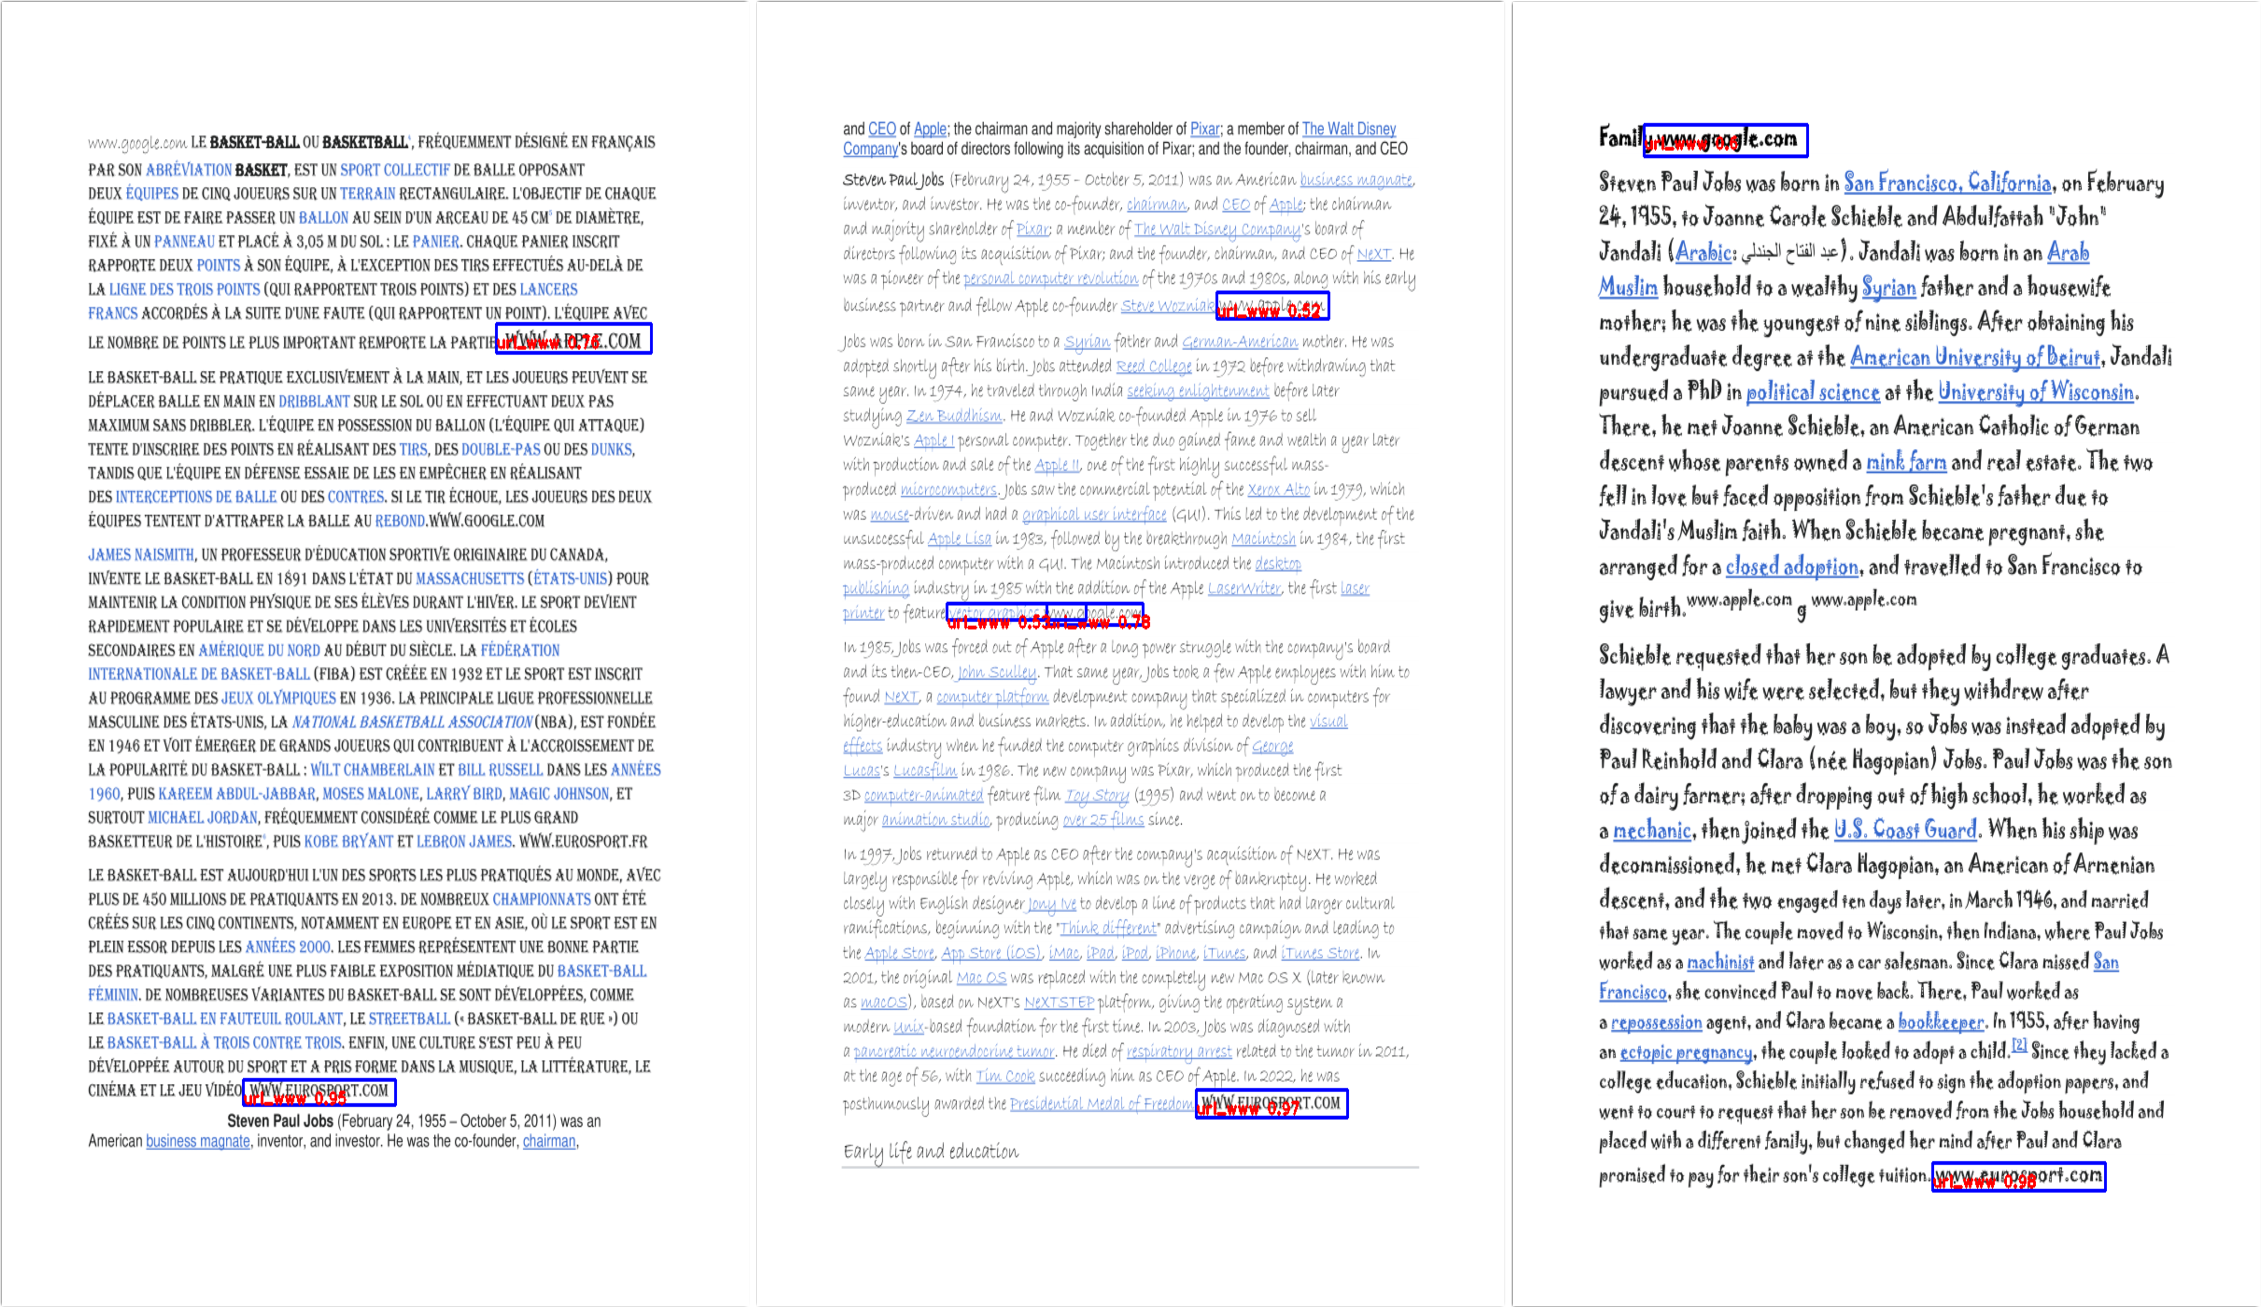
\includegraphics[height=9cm,width=17cm]{Chapitre3/font_yolov4.png}
                    \caption{Test de difficulté: Différentes polices de caractères - YOLOv4.}
                    \label{y4_t2}
                    \end{figure}
          \begin{figure}[H]
                    \centering
                    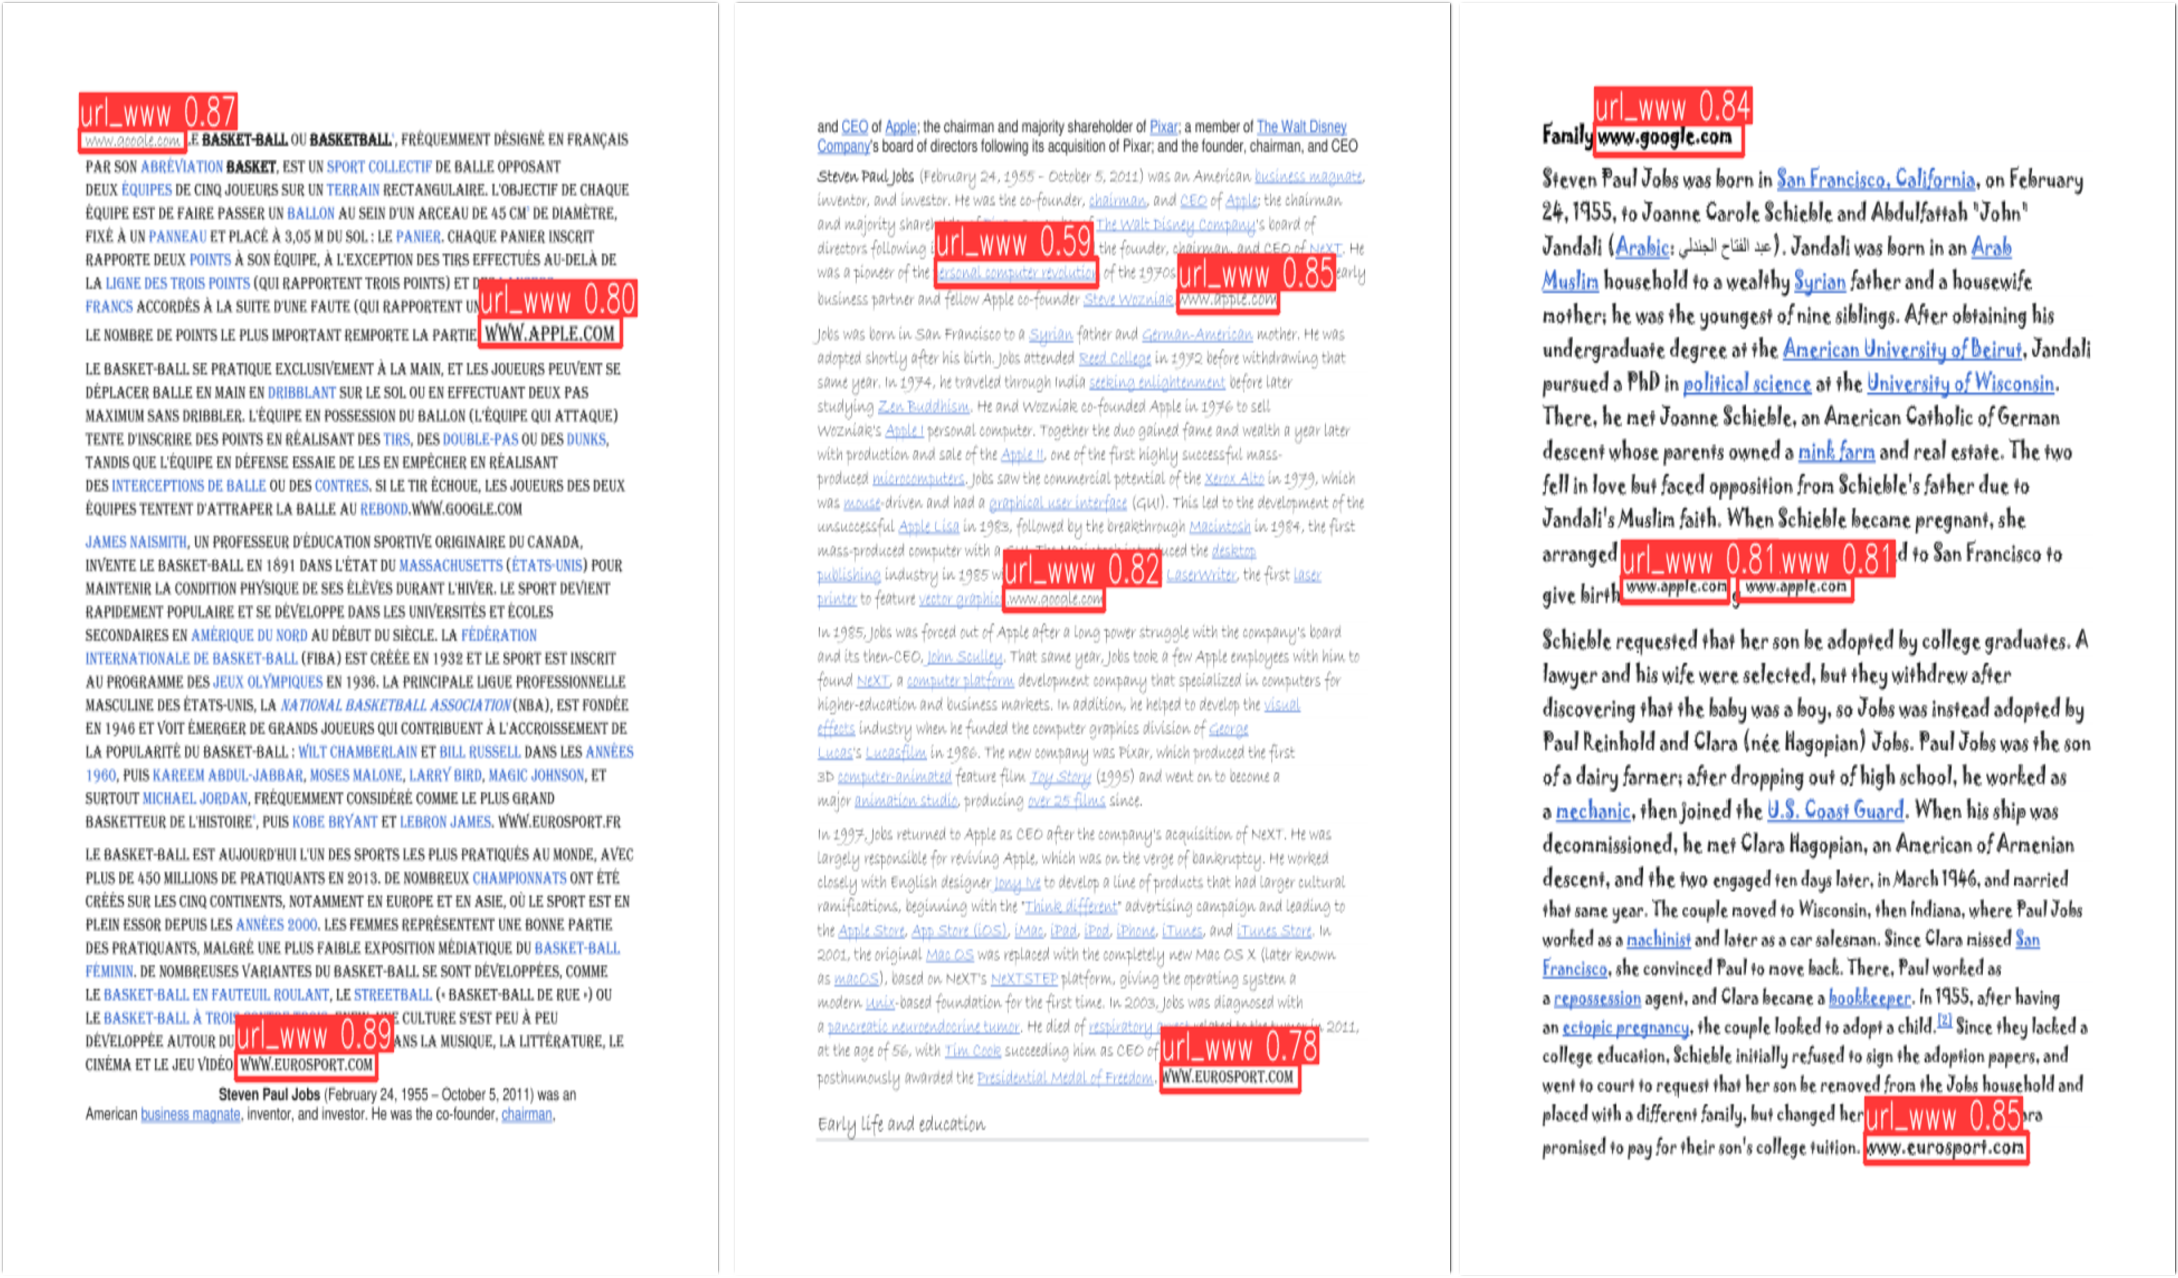
\includegraphics[height=9cm,width=17cm]{Chapitre3/font_yolov5.png}
                    \caption{Test de difficulté: Différentes polices de caractères - YOLOv5.}
                    \label{y5_t2}
                    \end{figure}

          % ---------- COLOR --------------
          \subsubsection{Différentes couleurs de fond et couleurs de caractères}
          Cette difficulté a fortement affecté les performances des modèles,
          YOLOv3 n'est pas capable de détecter les URL avec une couleur de fond colorée mais réussit à détecter les URL avec des caractères colorés, le modèle a obtenu $31,71\%$ de précision moyenne.
          YOLOv4 est le modèle performant dans cette difficulté avec une précision moyenne de $54,44\%$, il a réussi à détecter toutes les URL avec des caractères colorés et la plupart des URL avec un fond coloré.
          YOLOv5 est le moins performant de tous avec une précision moyenne de $27,27\%$ où il ne peut pas détecter complètement les URL avec des objets colorés et encore moins des arrière-plans colorés
          \begin{figure}[H]
               \centering
                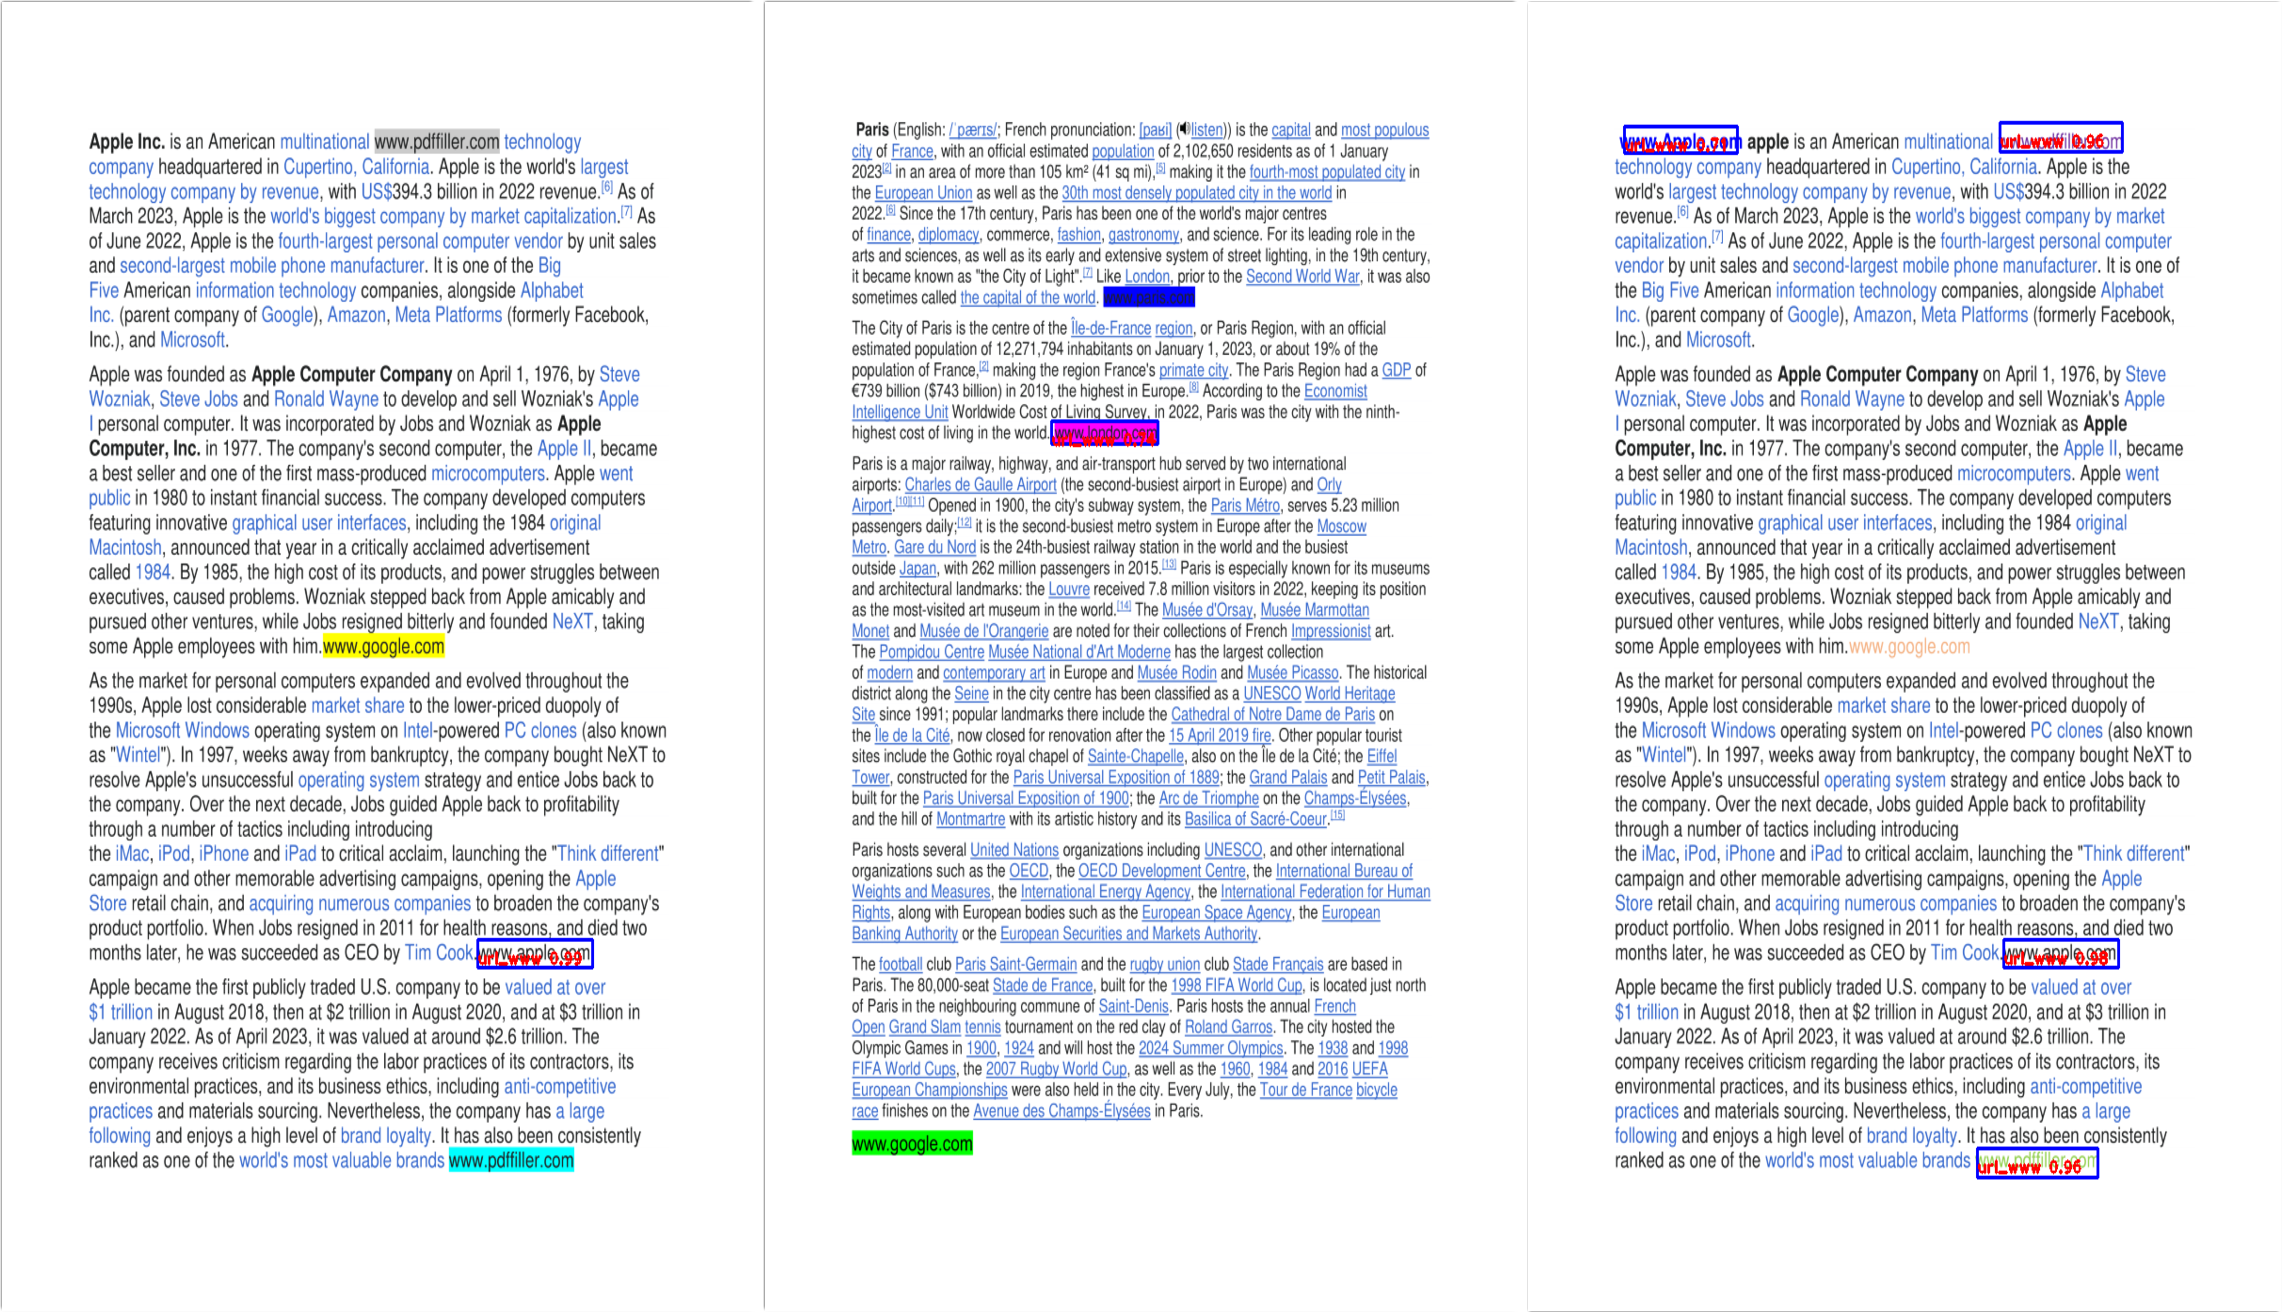
\includegraphics[height=9cm,width=17cm]{Chapitre3/color_yolov3.png}
                \caption{Test de difficulté: Différentes couleurs de fond et couleurs de caractères - YOLOv3.}
                \label{y3_t3}
                \end{figure}
          \begin{figure}[H]
                    \centering
                    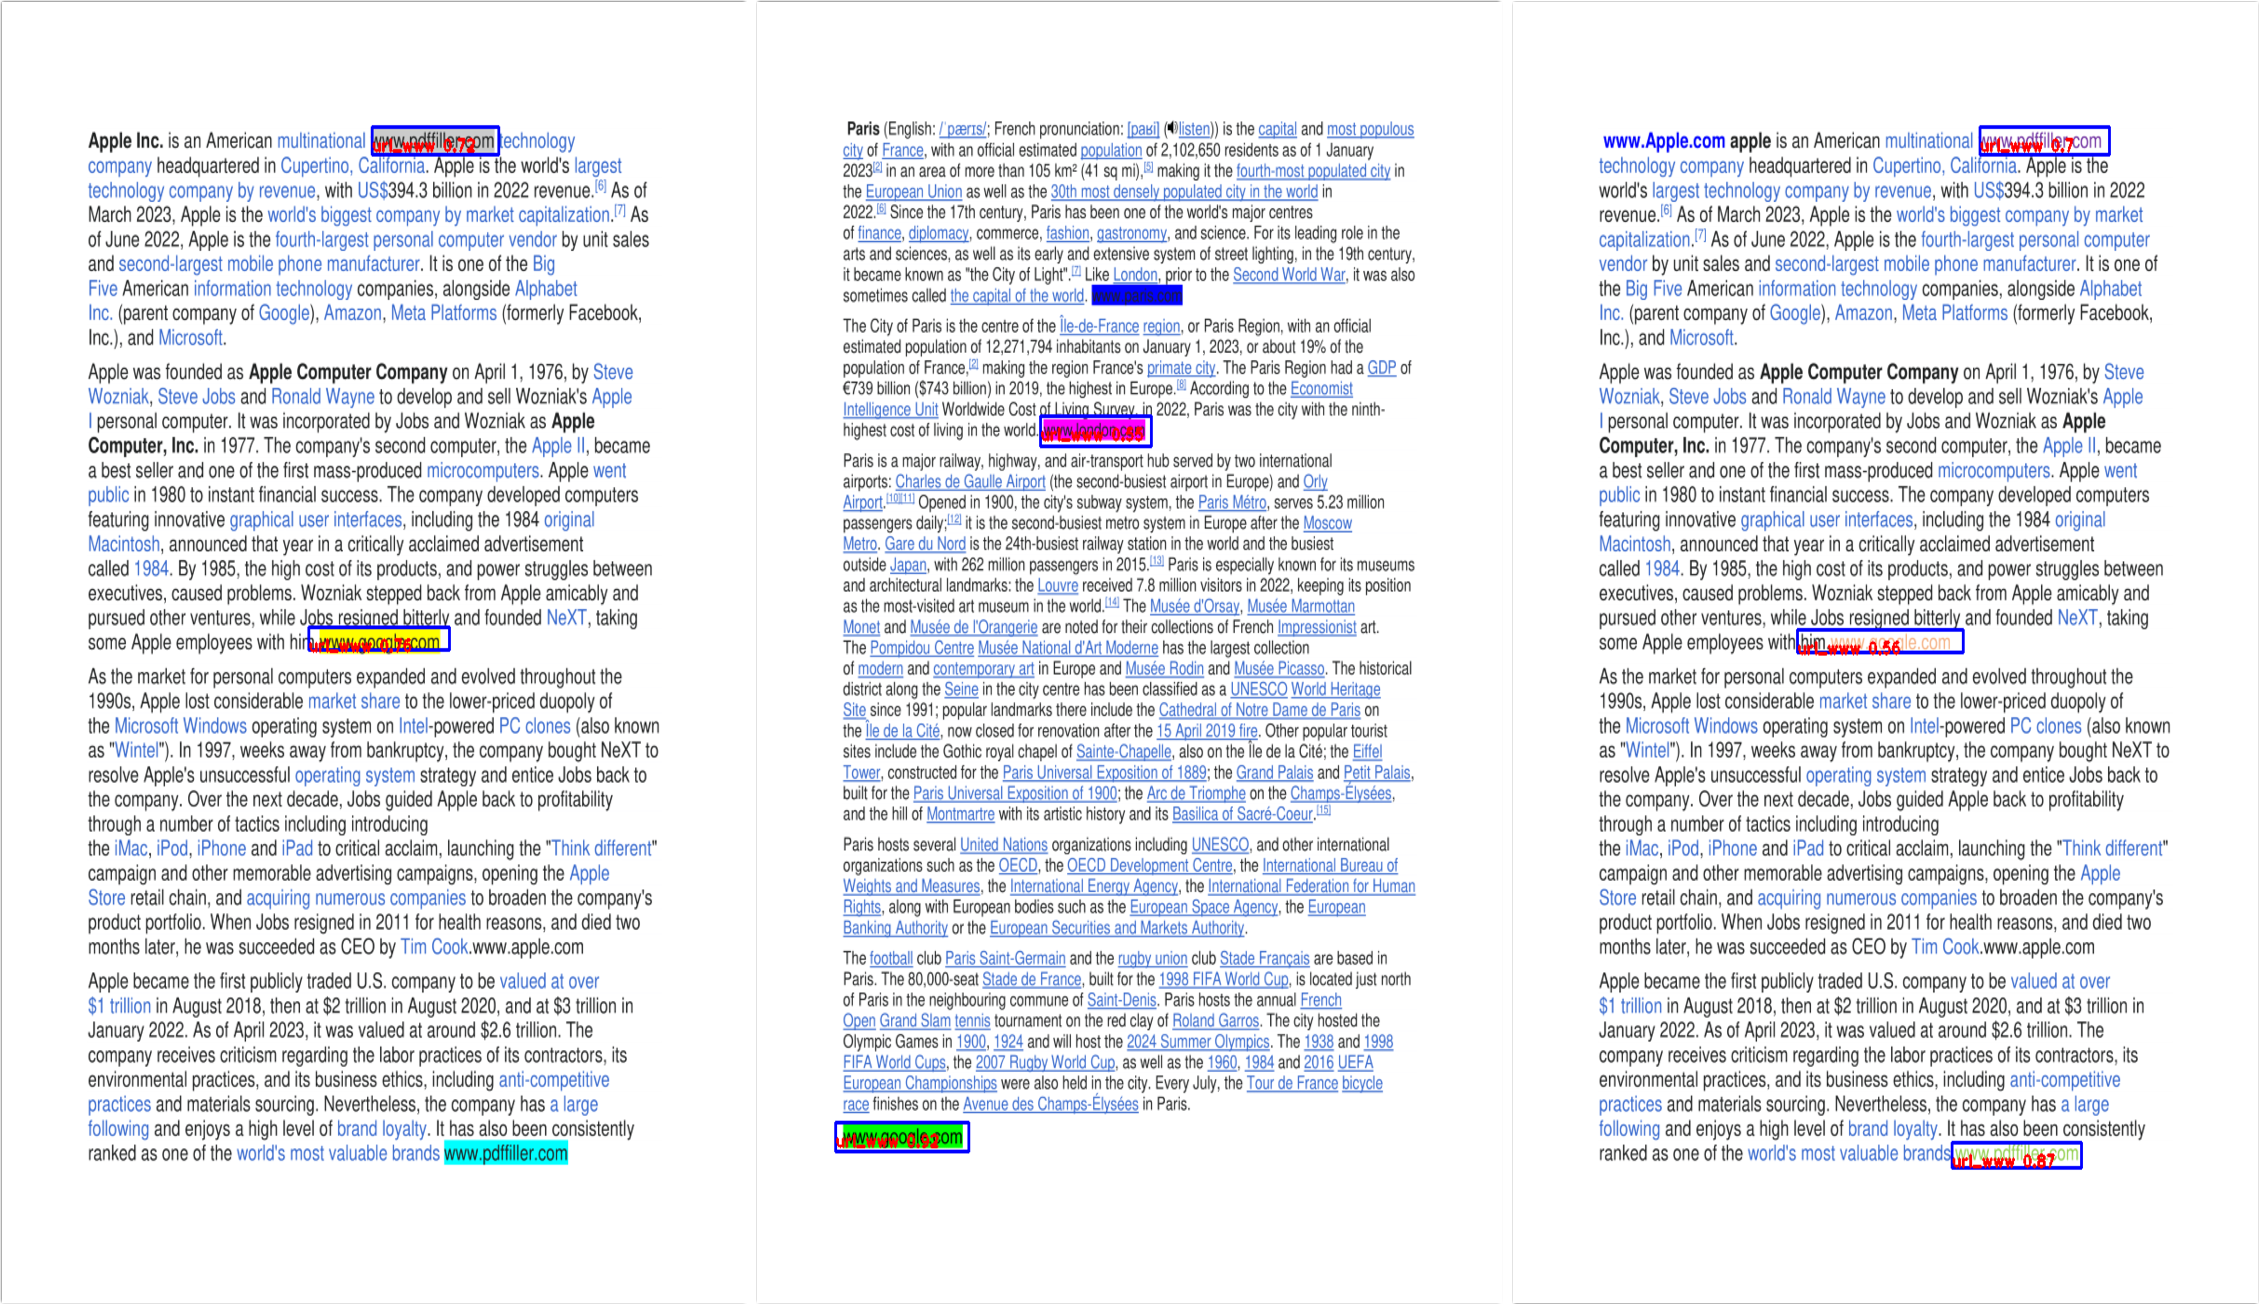
\includegraphics[height=9cm,width=17cm]{Chapitre3/color_yolov4.png}
                    \caption{Test de difficulté: Différentes couleurs de fond et couleurs de caractères - YOLOv4.}
                    \label{y4_t3}
                    \end{figure}
          \begin{figure}[H]
                    \centering
                    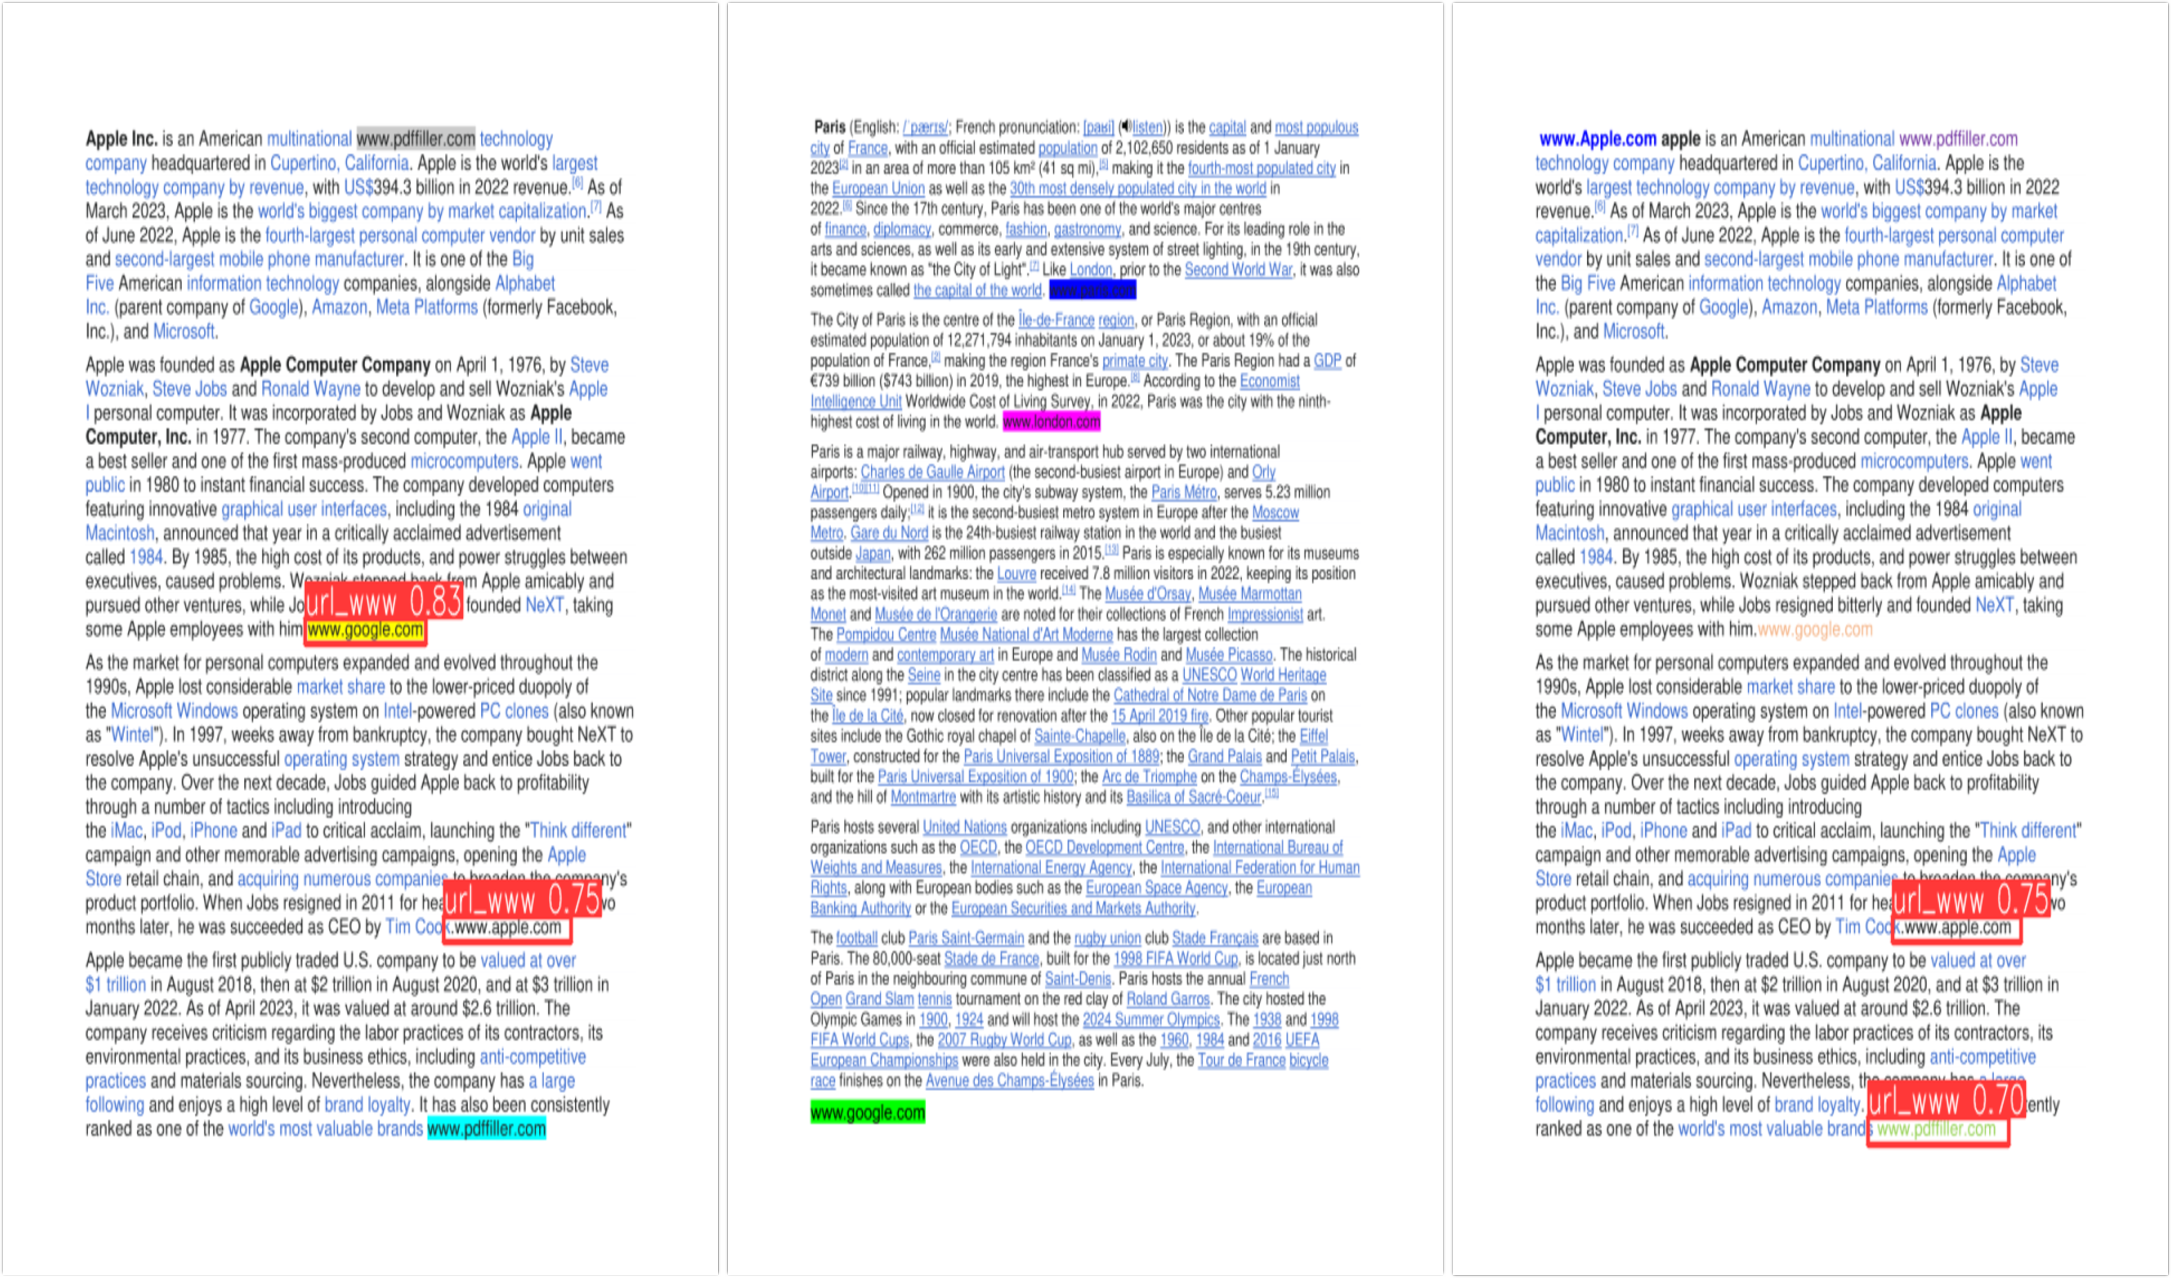
\includegraphics[height=9cm,width=17cm]{Chapitre3/color_yolov5.png}
                    \caption{Test de difficulté: Différentes couleurs de fond et couleurs de caractères - YOLOv5.}
                    \label{y5_t3}
                    \end{figure}
          
          % ---------- ROTATION --------------
          \subsubsection{Rotation des images sur $90^\circ$ et $180^\circ$}
          La rotation en $180^\circ$ n'a pas affecté les performances de tous les modèles comme cela ne s'est jamais produit. D'un autre côté, la rotation en $90\circ$ a totalement cassé les performances des modèles.
          \begin{figure}[H]
               \centering
                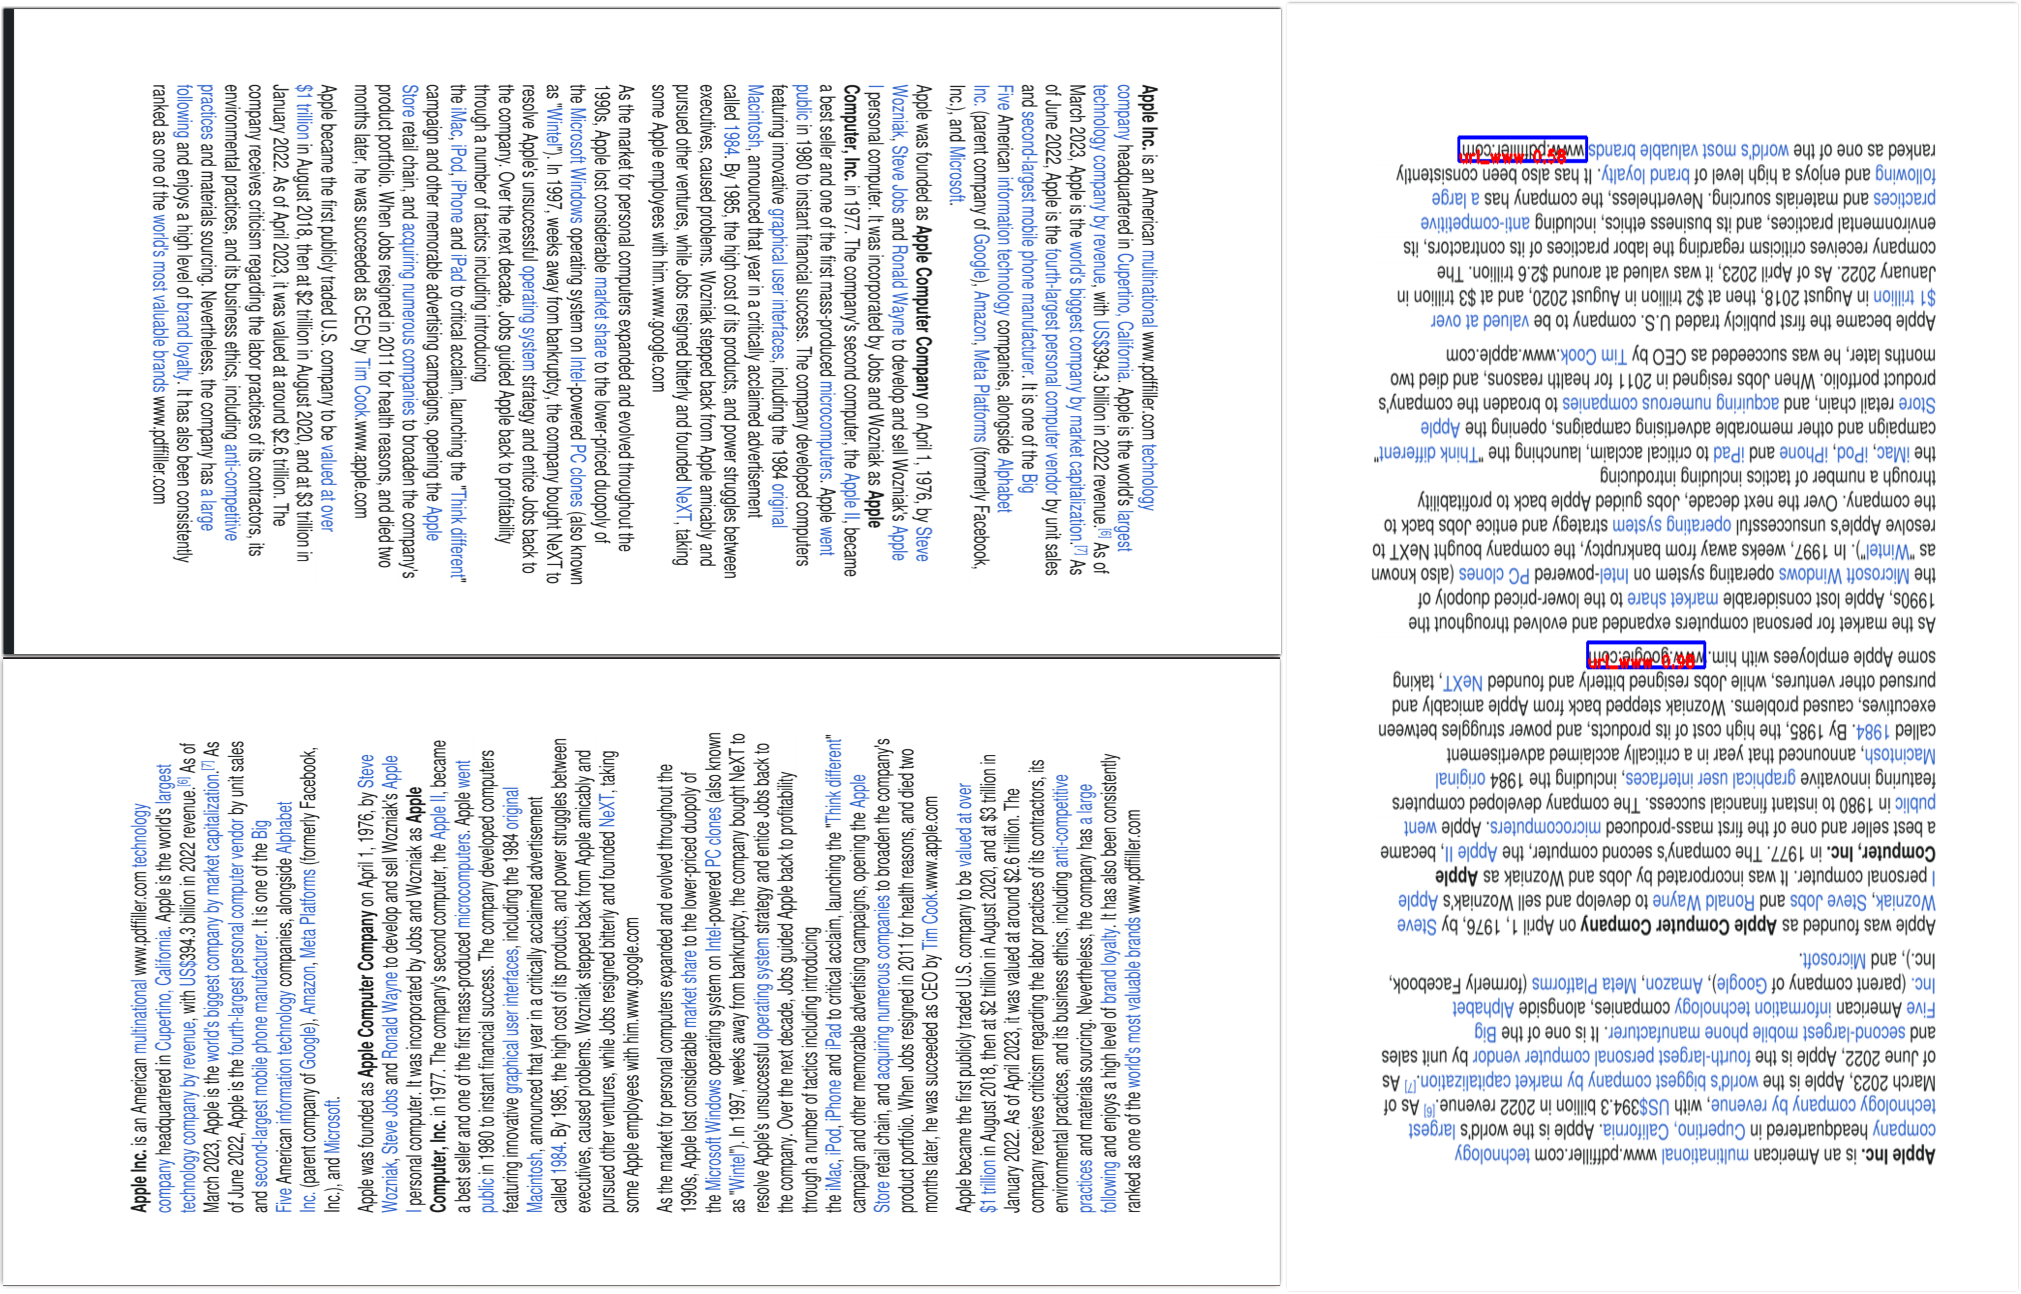
\includegraphics[height=12cm,width=17cm]{Chapitre3/rotation_yolov3.png}
                \caption{Test de difficulté: Rotation des images sur $90^\circ$ et $180^\circ$ - YOLOv3.}
                \label{y3_t5}
                \end{figure}
          \begin{figure}[H]
                    \centering
                    \includegraphics[height=12cm,width=17cm]{Chapitre3/rotation_yolov4.png}
                    \caption{Test de difficulté: Rotation des images sur $90^\circ$ et $180^\circ$ - YOLOv4.}
                    \label{y4_t4}
                    \end{figure}
          \begin{figure}[H]
                    \centering
                    \includegraphics[height=12cm,width=17cm]{Chapitre3/rotation_yolov5.png}
                    \caption{Test de difficulté: Rotation des images sur $90^\circ$ et $180^\circ$ - YOLOv5.}
                    \label{y5_t4}
                    \end{figure}

          % ---------- PROTOCOL-TAG --------------  
          \subsubsection{URL préfixées avec la balise de protocole \textit{https://}}
          La plupart des URL, tous les modèles n'ont pas réussi à les détecter et certains n'ont pas détecté l'URL complète (de la balise de protocole à l'extension), mais ils n'ont détecté que le nom de domaine uniquement.
          YOLOv3 a obtenu un score de $12,12\%$, YOLOv4 avait la précision la plus élevée avec $28,9\%$ et YOLOv5 $13,64\%$.
          \begin{figure}[H]
               \centering
                \includegraphics[height=9cm,width=17cm]{Chapitre3/https_yolov3.png}
                \caption{Test de difficulté: URL préfixées avec la balise de protocole \textit{https://} - YOLOv3.}
                \label{y3_t4}
                \end{figure}
          \begin{figure}[H]
                    \centering
                    \includegraphics[height=9cm,width=17cm]{Chapitre3/https_yolov4.png}
                    \caption{Test de difficulté: URL préfixées avec la balise de protocole \textit{https://} - YOLOv4.}
                    \label{y4_https}
                    \end{figure}
          \begin{figure}[H]
                    \centering
                    \includegraphics[height=9cm,width=17cm]{Chapitre3/https_yolov5.png}
                    \caption{Test de difficulté: URL préfixées avec la balise de protocole \textit{https://} - YOLOv5.}
                    \label{y5_https}
                    \end{figure}

          % ---------- MANUSCRIPT -----------
          \subsubsection{Caractères d'URL écrits en manuscrit}
          Tous les modèles ont échoué dans cette difficulté avec une précision moyenne de $0\%$.
          \begin{figure}[H]
                    \centering
                    \includegraphics[height=7cm,width=17cm]{Chapitre3/test_manuscript.png}
                    \caption{Test de difficulté: Images avec Flou-GaussianCaractères d'URL écrits en manuscrit - YOLOv3 / YOLOv4 / YOLOv5.}
                    \label{test_manuscrit}
                    \end{figure}

          % ---------- FLOU ------------
          \subsubsection{Images avec Flou-Gaussian.}
          Le flou n'affecte pas beaucoup les performances des modèles. YOLOv3 a obtenu une précision moyenne de $72,73\%$. YOLOv4 a obtenu un score parfait de $100\%$ et YOLOv5 un score de $90,91\%$.
          \begin{figure}[H]
                    \centering
                    \includegraphics[height=9cm,width=17cm]{Chapitre3/blur_yolov3.png}
                    \caption{Test de difficulté: Images avec Flou-Gaussian - YOLOv3.}
                    \label{y3_blur}
                    \end{figure}
          \begin{figure}[H]
                    \centering
                    \includegraphics[height=9cm,width=17cm]{Chapitre3/blur_yolov4.png}
                    \caption{Test de difficulté: Images avec Flou-Gaussian - YOLOv4.}
                    \label{y4_blur}
                    \end{figure}
          \begin{figure}[H]
                    \centering
                    \includegraphics[height=9cm,width=17cm]{Chapitre3/blur_yolov5.png}
                    \caption{Test de difficulté: Images avec Flou-Gaussian - YOLOv5.}
                    \label{y5_blur}
                    \end{figure}

          % ---------- FLOU ------------
          \subsubsection{Images avec Bruit-Gaussian.}
          Contrairement au flou, le bruit affecte grandement la précision des modèles, il amène les modèles à détecter de faux objets.
          La précision YOLOv3 a chuté à $36,36\%$ et YOLOv4 a également chuté au même score de $36,36\%$. Contrairement aux deux, YOLOv5 a obtenu un score plus élevé de $83,98\%$.
          \begin{figure}[H]
                    \centering
                    \includegraphics[height=9cm,width=17cm]{Chapitre3/bruit_yolov3.png}
                    \caption{Test de difficulté: Images avec Bruit-Gaussian - YOLOv3.}
                    \label{bruit_y3}
                    \end{figure}
          \begin{figure}[H]
                    \centering
                    \includegraphics[height=9cm,width=17cm]{Chapitre3/bruit_yolov4.png}
                    \caption{Test de difficulté: Images avec Bruit-Gaussian - YOLOv4.}
                    \label{bruit_y4}
                    \end{figure}
          \begin{figure}[H]
                    \centering
                    \includegraphics[height=9cm,width=17cm]{Chapitre3/bruit_yolov5.png}
                    \caption{Test de difficulté: Images avec Bruit-Gaussian - YOLOv5.}
                    \label{bruit_y5}
                    \end{figure}

          % ---------- SCREENSHOT ------------

\section{Conclusion Géneral}
%\input{Chapitre4/Chapitre4.tex}
%\chapter*{Conclusion générale}
\pagestyle{fancy}
\fancyhead[L]{}
\fancyhead[R]{Conclusion générale}
\renewcommand{\headrulewidth}{1pt}
\fancyfoot[C]{\thepage}
\section*{Conclusion générale}
Dans ce travail, nous avons étudié un thème très abordé en détection d'objets et apprentissage profond qui s'applique  sur ensemble des images, 

Dans le cadre de ce mémoire, premièrement nous avons présenté la  définition  de la détection  d'objets  et ses  applications.

ensuite, nous avons introduit  les modèles de détection d'objets  (3 méthodes ) avant Période de détection par apprentissage profond (après 2014 ) ,dans cette période  la détection d'objets est regroupée en deux classes : la "détection en deux étapes (RCNN-SPP NET -FPN)" et la "détection en une étape (YOLO-SSD)".

Également, nous avons présenté  les Mesures d'évaluation des systèmes de détection d'objets. 

Enfin, nous décrivons la création de l'ensemble de données et les différentes étapes d'apprentissage à l'aide de YOLOv3, YOLOv4 et YOLOv5, ainsi que les résultats des tests.

Notre objectif était de mettre en place une architecture permettant reconnaissance d’url dans différents difficultés.

Les résultats expérimentaux exprimés en terme de plusieurs métriques dans le domaine   de la reconnaissance  d’url, nous a permis de déduire les conclusions suivantes:
\paragraph{-} Les 3 modèles ont donné des résultats très satisfaisants dans le test de la base de données, mais le meilleur est YOLOv4. 
\paragraph{-} Les 3 modèles ont donné $0.0\%$ (AP) dans le test de rotation à $90^\circ$.
\paragraph{-} Les 3 modèles ont donné $0,0\%$ (AP) au test du Manuscrit.

pour améliorer les résultats , nous proposons de : 

\paragraph{-} D’augmenter la taille de l'ensemble de données.
\paragraph{-}ajouter des images avec des difficultés à l'ensemble de données.
\paragraph{-} D’améliorer et d'ajouter le nombre d'itérations dans la phase d’apprentissage.
\paragraph{-} Utiliser les nouvelles versions de YOLO et comparer les résultats.



%\chapter*{Bibliographie}
\pagestyle{fancy}
\fancyfoot[C]{\thepage}
\newpage
 \addcontentsline{toc}{chapter}{Bibliographie}
\bibliographystyle{plain} %plain
\bibliography{Bibliographie/references} 
%-----------------Fin Zone 5: fin de la numérotation avec les chiffres arabs---------------------
\backmatter 
%\input{Annexe/Annexe.tex}
\addcontentsline{toc}{chapter}{Annexe}

\end{document}